\documentclass[10pt, conference, letterpaper]{IEEEtran}

\usepackage{algorithm}
\usepackage{algorithmicx}
\usepackage{algpseudocode}
\usepackage{amsfonts}
\usepackage{amsmath}
\usepackage{amssymb}
\usepackage[ansinew]{inputenc}
% \usepackage[utf8]{inputenc} % why not
\usepackage{xcolor}
\usepackage{mathtools}
\usepackage{graphicx}
\usepackage{caption}
\usepackage{subcaption}
\usepackage{import}
\usepackage{multirow}
\usepackage{cite}
\usepackage[export]{adjustbox}
\usepackage{breqn}
\usepackage{mathrsfs}
\usepackage{acronym}
%\usepackage[keeplastbox]{flushend}
\usepackage{setspace}
\usepackage{bm}
\usepackage{stackengine}

\usepackage{tikz}
\usetikzlibrary{calc}

\usepackage{listings}

\lstset{%
    backgroundcolor=\color[gray]{.85},
    basicstyle=\small\ttfamily,
    breaklines = true,
    keywordstyle=\color{red!75},
    columns=fullflexible,
}%

\lstdefinelanguage{BibTeX}
{keywords={%
        @article,@book,@collectedbook,@conference,@electronic,@ieeetranbstctl,%
        @inbook,@incollectedbook,@incollection,@injournal,@inproceedings,%
        @manual,@mastersthesis,@misc,@patent,@periodical,@phdthesis,@preamble,%
        @proceedings,@standard,@string,@techreport,@unpublished%
    },
    comment=[l][\itshape]{@comment},
    sensitive=false,
}

\usepackage{listings}

% listings settings from classicthesis package by
% Andr\'{e} Miede
\lstset{language=[LaTeX]Tex,%C++,
    keywordstyle=\color{RoyalBlue},%\bfseries,
    basicstyle=\small\ttfamily,
    %identifierstyle=\color{NavyBlue},
    commentstyle=\color{Green}\ttfamily,
    stringstyle=\rmfamily,
    numbers=none,%left,%
    numberstyle=\scriptsize,%\tiny
    stepnumber=5,
    numbersep=8pt,
    showstringspaces=false,
    breaklines=true,
    frameround=ftff,
    frame=single
    %frame=L
}

\renewcommand{\thetable}{\arabic{table}}
\renewcommand{\thesubtable}{\alph{subtable}}

\DeclareMathOperator*{\argmin}{arg\,min}
\DeclareMathOperator*{\argmax}{arg\,max}

\def\delequal{\mathrel{\ensurestackMath{\stackon[1pt]{=}{\scriptscriptstyle\Delta}}}}

\graphicspath{{./figures/}}
\setlength{\belowcaptionskip}{0mm}
\setlength{\textfloatsep}{8pt}

\newcommand{\eq}[1]{Eq.~\eqref{#1}}
\newcommand{\fig}[1]{Fig.~\ref{#1}}
\newcommand{\tab}[1]{Tab.~\ref{#1}}
\newcommand{\secref}[1]{Section~\ref{#1}}

\newcommand\MR[1]{\textcolor{blue}{#1}}
\newcommand\red[1]{\textcolor{red}{#1}}
\newcommand{\mytexttilde}{{\raise.17ex\hbox{$\scriptstyle\mathtt{\sim}$}}}

%\renewcommand{\baselinestretch}{0.98}
% \renewcommand{\bottomfraction}{0.8}
% \setlength{\abovecaptionskip}{0pt}
\setlength{\columnsep}{0.2in}

% \IEEEoverridecommandlockouts\IEEEpubid{\makebox[\columnwidth]{PUT COPYRIGHT NOTICE HERE \hfill} \hspace{\columnsep}\makebox[\columnwidth]{ }}

\title{Speech Command Recognition}

\author{pmn}

\IEEEoverridecommandlockouts

\newcounter{remark}[section]
\newenvironment{remark}[1][]{\refstepcounter{remark}\par\medskip
\textbf{Remark~\thesection.\theremark. #1} \rmfamily}{\medskip}

\begin{document}

\maketitle

\begin{abstract} This report covers the work done to solve the speech command
    recognition task, following four approaches: a convolutional neural
    network, transfer learning using a pre-trained image-classifying
    architecture, a recurrent attention model, and a convolutional attention
    model.
    % att query
    A different method to compute the attention weight for the recurrent model
    is tested, using convolutional layers to compute the scores, both directly
    from the spectrogram and from the LSTM features.
    % hypa
    Experiments to identify the best input preprocess and model
    hyper-parameters are performed for the four architectures.
    % Streaming: keyword spotting adaptation of the model
    The models' performances were tested in an online fashion, evaluating the
    keyword spotting capabilities on an audio stream.
    % results
    The convolutional+attention model reached 99.88\% accuracy on the ``yes/no''
    task, 98.64\% on a 10+2 task composed of 10 words, one silence, and one
    background conversation classes; and 95.72\% on the 35+2 task that contains
    all the available words.
\end{abstract}

\IEEEkeywords
Keyword Spotting,
Attention Mechanism
\endIEEEkeywords

% !TEX root = report.tex

\section{Introduction}
\label{sec:introduction}

% A fascinating introduction
% Never forget \cite{2018arXiv180808929C}

Keyword Spotting or Voice Command Recognition are key components that allow
speech based user interaction.
%
Many smart devices use a specific wake phrase to initiate the active
interaction with the user (e.g. ``Ok Google'', ``Alexa''), while other devices
are controlled by specific voice commands (e.g. ``play'', ``stop'', ``lights
off'').
%
Other automated services might respond to the user's voice, for example to
collect data during an automated telephone survey.
%
A pre-defined set of keywords must be identified within a continuos stream of
audio. Several properties are desired in the model that analyzes the audio: low
energy consumption to account for the ``always-on'' performance, that stands
alongside with a small memory footprint to allow the use of the model on
embedded devices, and with a low latency in the reaction, to provide a fluid
user experience.
%
These properties allow for the model to be run locally, and to only send audio
to a cloud-based system, with far higher computational capability, only after
waking up the device, to address the more complex interaction that follows.

% Control a device with voice command (play, stop, lights off)
% wake words
% initiate interaction
% continuos stream of audio
% predefined set of words
% auto no hands
% automated surveys
% low energy consumption
% low memory
% always on - cloud - latency - real time response
% low resources devices or micro-controllers

attention selectively focus on portion of the inputs

attention wide variety of tasks 



% !TEX root = report.tex

\section{Related Work}
\label{sec:related_work}

% MFCC + HMM
The first classification models used Mel Frequency Cepstral Coefficients to
compactly extract features from the audio signal and a Hidden Markov model to
compute the prediction, leveraging the HMM ability of modelling sequences
\cite{mfcchmm103088}.
% ConvNets
Deep Neural Networks, in more recent years, provided efficient solutions
\cite{chensmallDNN} and Convolutional Neural Networks have been successfully
applied to exploit the spatial correlations in the spectrograms while keeping a
small memory footprint for the model \cite{sainathconvolutional}.
% RNN
Long short-term memory cells are used to better deal with long time
dependencies within the signal, allowing some delay in the decision while
keeping an internal state that acts as memory \cite{fernandezRNNKWS}.

% Attention mechanism
The attention mechanism allows the model to selectively focus on some portions
of the input data that is judged to be more relevant.
% Attention wide variety of tasks 
This mechanism has been applied successfully to a variety of tasks, such as
machine translation \cite{luong2015effective}, \cite{bahdanau2016neural}, and
image caption generation \cite{xu2016show}.
% Andrade
The attention mechanism was adapted to the speech commands recognition task
\cite{2018arXiv180808929C}, where it was used in conjunction to LSTMs focusing
on single word recognition.
% Federated learning for privacy concerns
A federated learning approach can be used to train a central model on the local
data of many users \cite{leroy2019federated}, addressing concerns regarding the
privacy of the training data.
% Microcontrollers
The power and memory requirements, are carefully investigated in
\cite{zhang2018hello}, where a resource constrained neural network architecture
exploration is performed, to maximize the performances within a given set of
constraints. On top of that, Neural Network Quantization is used to shrink the
otained models even more, using the quantization technique presented in
\cite{10.1145/2847263.2847265}.
% Tsetlin Machines
A completely different learning framework is used in \cite{granmo2021tsetlin},
where a learning algorithm called the Tsetlin Machine is applied.
The core of this machine is the Tsetlin Automaton,
that uses a penalty/reward signal to train the automaton, whose decisions are
combined with a clause module to create logic propositions that describe the 
input features.
% A learning automata powered machine is used to 
Application-specific integrated circuit (ASIC) exist for this architecture,
allowing for extremely energy-efficient inference.
% Tsetlin machine (TM) is evaluated in the KWS-AI design in place of the
% traditional perceptron based NNs. The machine operates through deriving
% propositional logic that describes the input features. It has shown great
% potential over NN based models in delivering energy frugal AI application
% while maintaining faster convergence and high learning efficacy


% !TEX root = report.tex

\section{Processing Pipeline}
\label{sec:processing_architecture}

High level descripion of the processing flow:

Throughout the report: extract Spectrograms, classify image.

\section{Signals and Features}
\label{sec:model}

\subsection{Google Dataset}

% Measurement setup, data preprocess (describe the google dataset)

The Speech Commands datasets, described in \cite{warden2018speech}, provides
thousands of one second recording of $35$ differen words. The recordings are
mainly of volounteers, who used their own device to record the words in a
closed room wherever they happened to be (not in a studio setting).
Ideally each volounteer only recorded the $135$ requested utterances once, so the
dataset provides good variability of voices.
The utterances have a duration of one second.
To more precisely align the recorded clips, the audio was acquired for $1.5$
seconds and the $1$ second clip that contained the highest overrall volume was
extracted.
Several background noise recording are included as well.
The full dataset includes $105829$ utterances of $35$ words, saved in
\textit{.wav} format at $16$ KHz rate.
The dataset is released under the Creative Commons BY $4.0$ License \cite{ccby4}.

The dataset ships with a function to split the data in train, validation and
test folds, as well as two example lists of validation data ($9981$ utterances)
and test data ($11005$ utterances).
Throughout the experiments, those lists were used.
% MAYBE both for the practicality of having them ready, but also to keep with
% the spirit of the dataset as a tool to enable meaningf

% TODO: how the words are grouped, tell the keys

Smaller tasks were used to evaluate the performance of the various
architectures, and to perform the hyper-parameter search.
Two 4 words task are composed by the words
[\texttt{happy}, \texttt{learn}, \texttt{wow}, \texttt{visual}],
[\texttt{backward}, \texttt{eight}, \texttt{go}, \texttt{yes}].
A 6 words task contains the direction words:
[\texttt{up}, \texttt{down}, \texttt{forward}, \texttt{backward},
\texttt{left}, \texttt{right}]
Two 10 words task contains the number utterances:
[\texttt{zero}, \texttt{one}, \texttt{two}, \texttt{three}, \texttt{four},
\texttt{five}, \texttt{six}, \texttt{seven}, \texttt{eight}, \texttt{nine}]
and the words from a Kaggle competition aimed at solving this task:
[\texttt{yes}, \texttt{no}, \texttt{up}, \texttt{down}, \texttt{left},
\texttt{right}, \texttt{on}, \texttt{off}, \texttt{stop}, \texttt{go}]
and a 20 words task is composed by the numbers and the Kaggle list.

\subsection{Mel spectrogram and Mel-frequency Cepstral Coefficients}

The audio data in the dataset is available as a vector of amplitudes over time,
sampled at $16$ KHz. In this representation, the classification task is quite
hard.
The Fourier transform allows to convert a signal from the time domain into the
frequency domain. The result is called spectrum of the signal. This transform
is efficiently computed using the Fast Fourier Transform algorithm.

The short-time Fourier transform accounts for variations of the content of an
audio signal over time. Instead of computing the FFT of the entire signal, the
FFT is computed on overlapping windowed segments of the signal: each window has
length \texttt{n\_fft} and the next window is extracted after
\texttt{hop\_length} samples.
The results of the FFT in each window are stacked to obtain the spectrogram.

The human ear does not perceive frequencies on a linear scale: the difference
between $200$ and $400$ Hz is very marked, whereas two notes at $8000$ and
$8200$ Hz are almost indistinguishable. The mel scale, proposed by Stevens,
Volkmann, and Newmann \cite{melscale1937}, introduces a unit of pitch built in
such a way that equal distances on the scale sound equally distant to the human
listener.
The mel spectrogram is a spectrogram where the frequencies are converted to the
mel scale. To do so, a Mel spaced filterbank is generated (a 10 filters version
is shown in \fig{fig:mel10_filterbank}) and the FFT results are multiplied with
a dot product with each filter, obtaining \texttt{n\_mel} values for each
timestep.

\begin{figure}[t!]
    \centering
    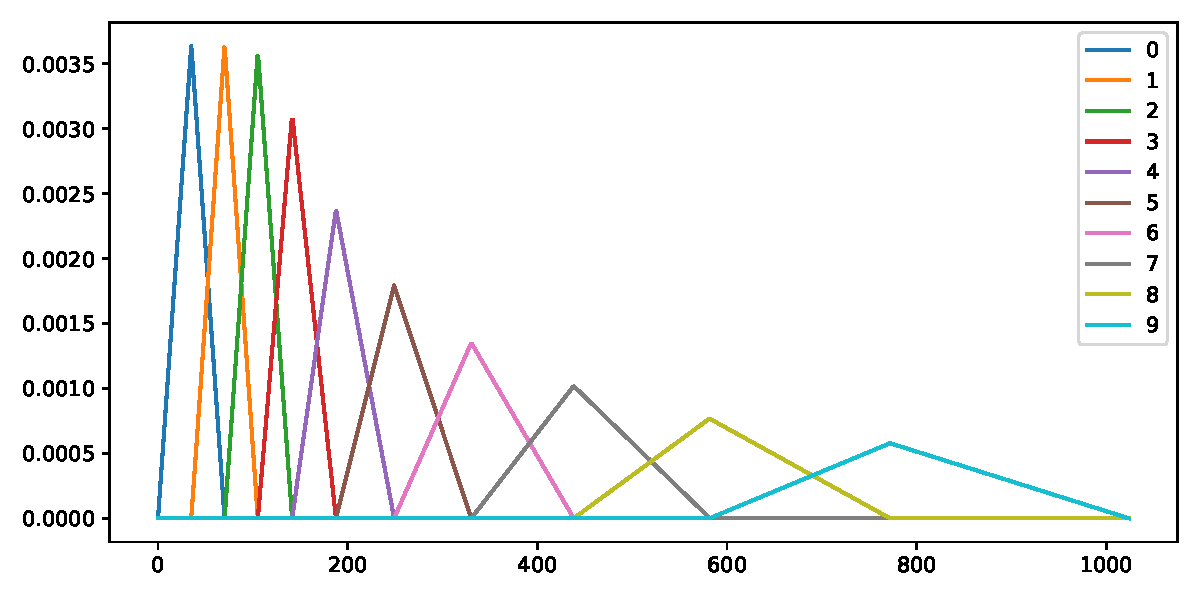
\includegraphics[width=0.9\linewidth]{mel10_filterbank.pdf}
    \caption{An example of a 10 filters Mel filterbank}
    \label{fig:mel10_filterbank}
\end{figure}

The resulting coefficients are highly correlated: the Discrete Cosine Transform
can be applied to decorrelate the filter bank coefficients and obtain a
compressed representation.
The results are the Mel-frequency Cepstral Coefficients.

The spectrograms were obtained using the \texttt{librosa} library
\cite{brian_mcfee_2020_3955228}.
The values used to generate the mel spectrograms are listed in
\tab{tab:mel_values}.
The values used to generate the mel frequency cepstral coefficients are listed
in \tab{tab:mfcc_values}.
An example waveform for the word ``happy'' and the relative spectrograms are
shown in \fig{fig:happy_specs}.

Some of the architectures that were tested require a square image as input,
with three color channels.
To obtain them, some spectrogams were purposefully generated with parameters
that created a square result, others, shaped like a half square, were
concatenated, as shown in the ``melc1'' spectrogram in
\fig{fig:happy_mel01_mel04_mel06_melc1_specs}.
Three square spectrogams are then stacked depthwise to obtain a valid three
channel image.
The values used to compose the spectrogams are listed in \tab{tab:compose_values}.
The values used to stack the spectrogams are listed in \tab{tab:ch3_values}.

\begin{figure}[t!]
    \centering
    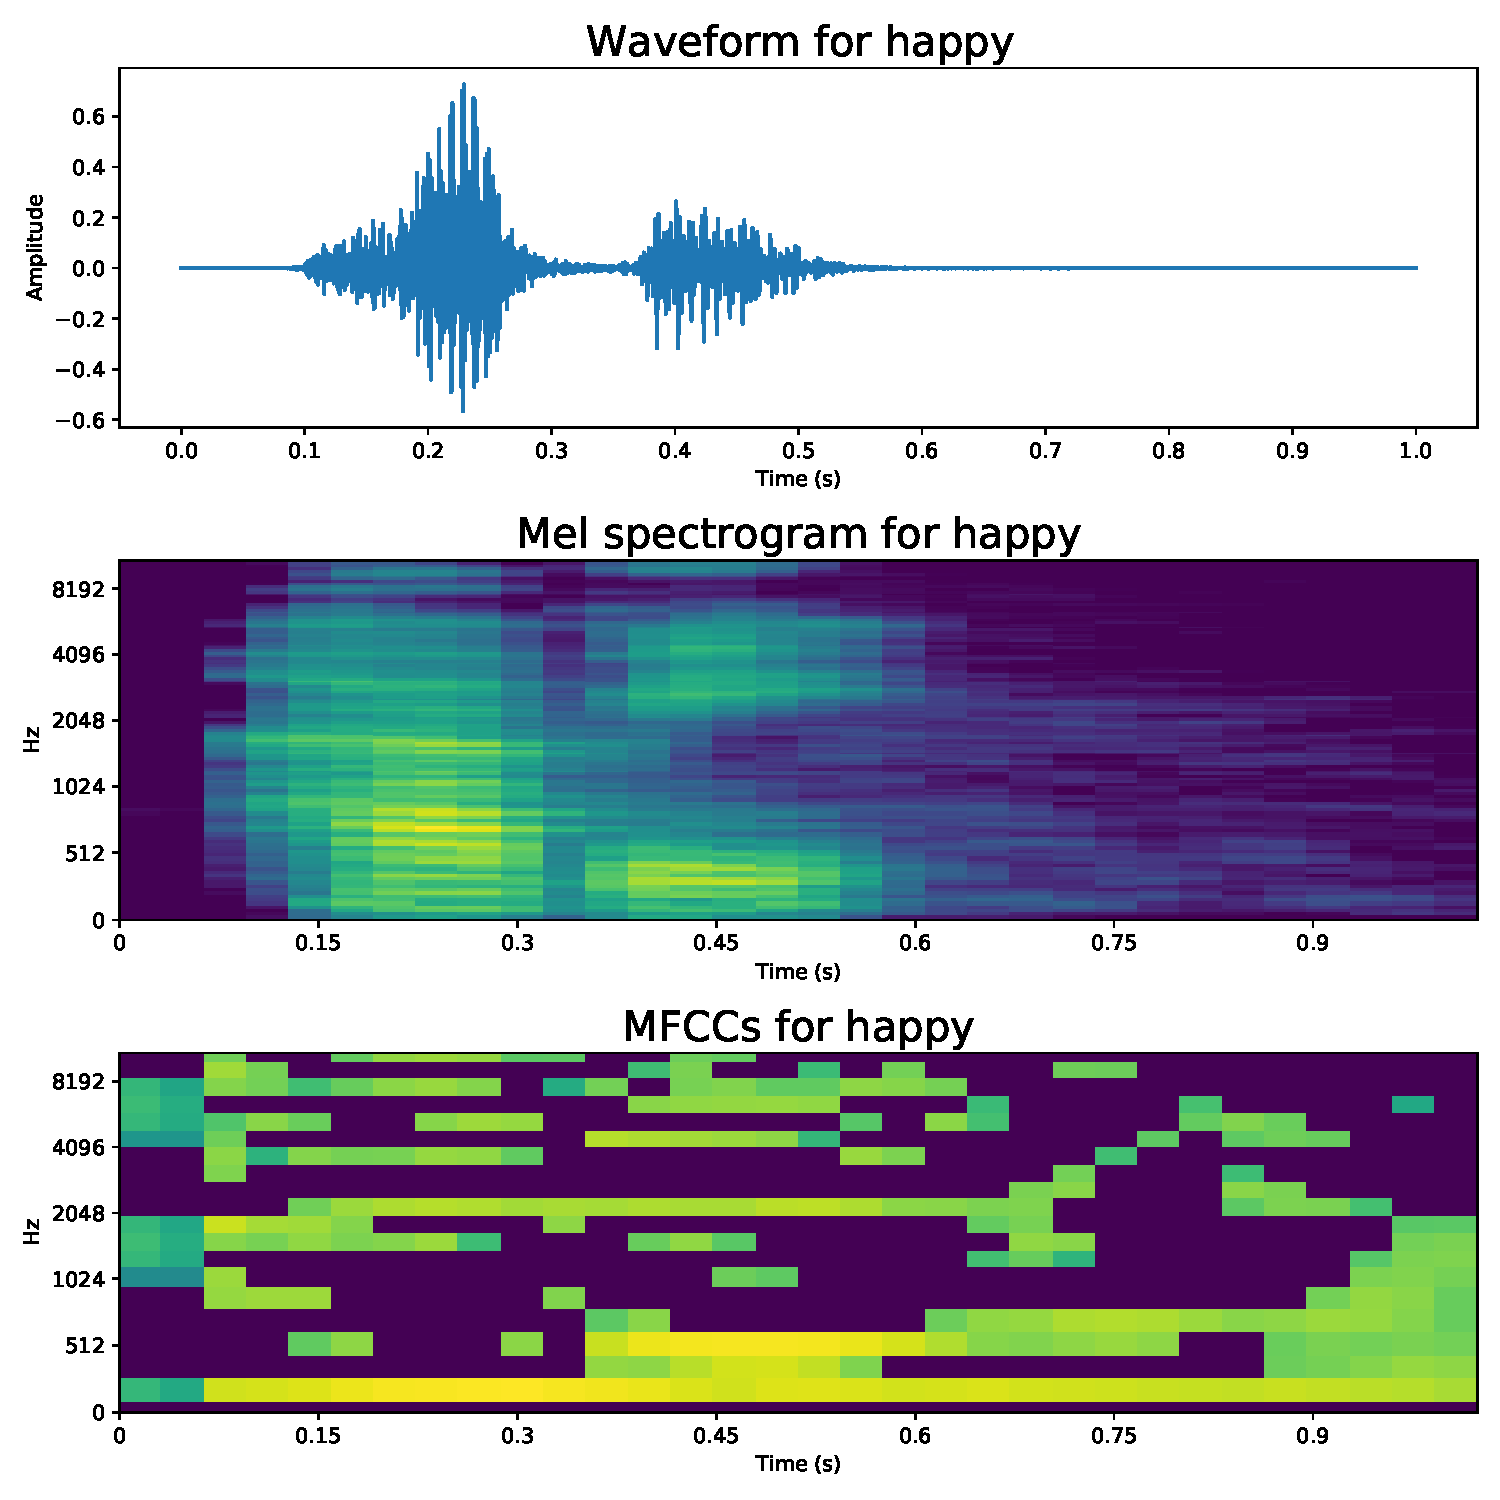
\includegraphics[width=0.9\linewidth]{happy_specs.pdf}
    \caption{
    Waveform and spectrograms for the word happy. Note that the y axis of the
spectrograms are labeled as Hz, but this is only to read more easily the plot
and understand to which frequencies the important bins correspond to. }%
    \label{fig:happy_specs}
\end{figure}

\begin{figure}[t!]
    \centering
    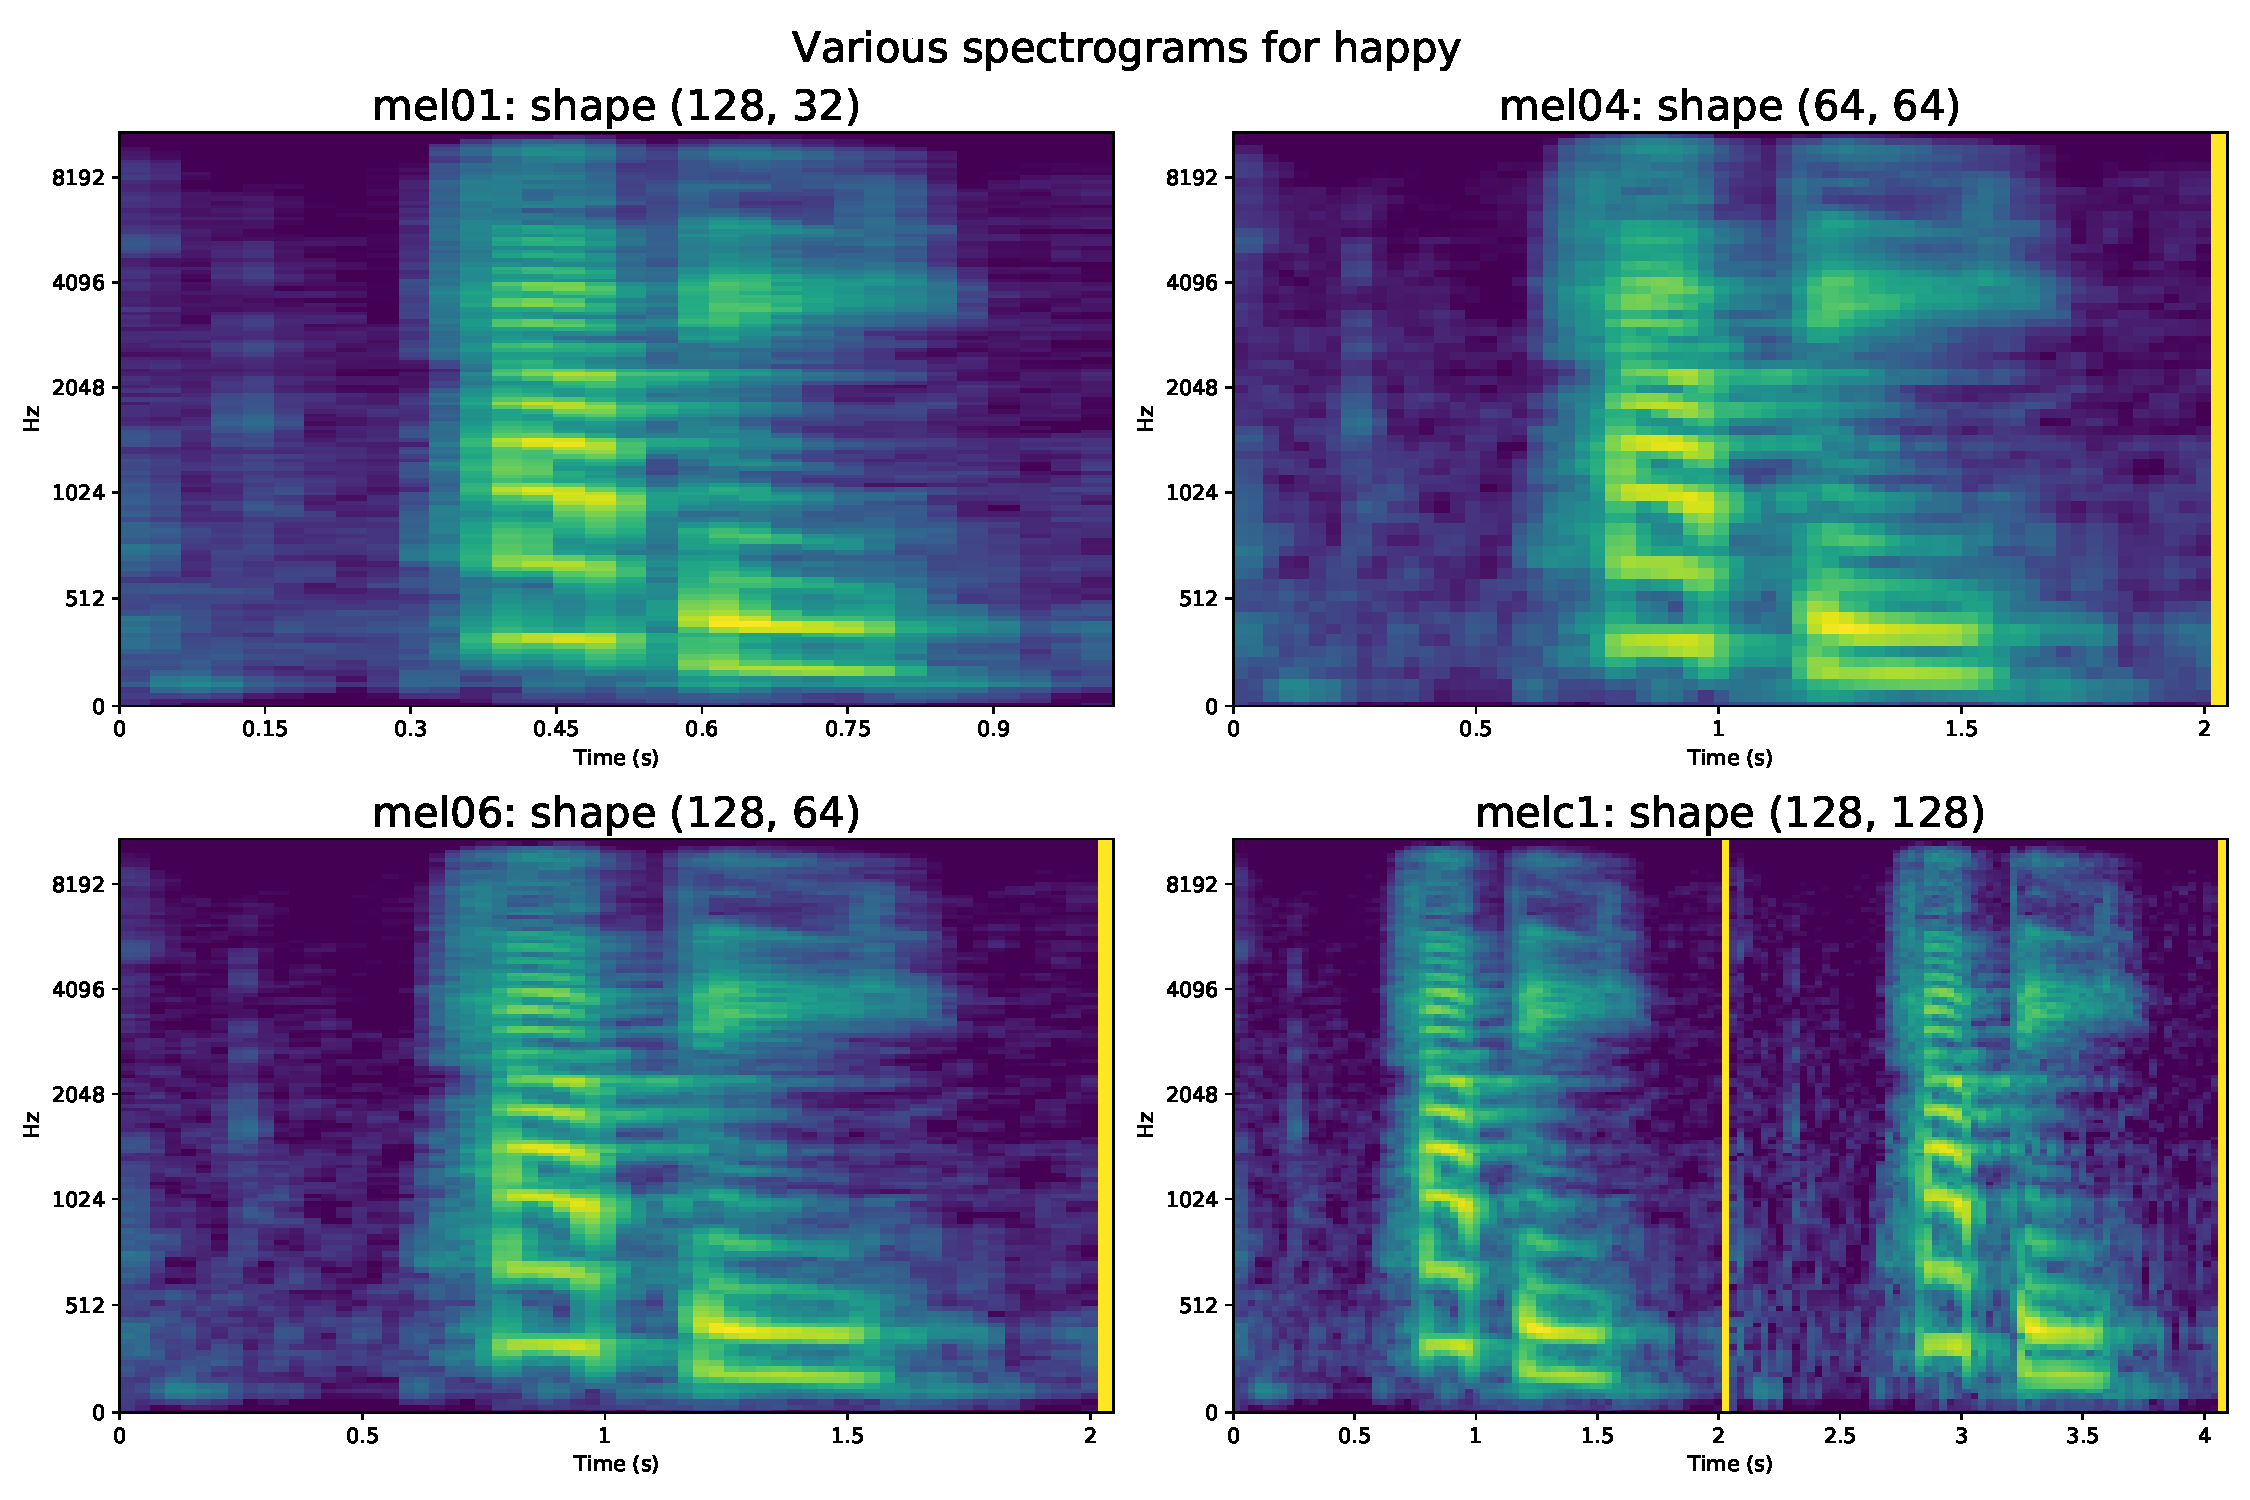
\includegraphics[width=0.9\linewidth]{happy_mel01_mel04_mel06_melc1_specs.pdf}
    \caption{Different spectrograms for the same word}%
    \label{fig:happy_mel01_mel04_mel06_melc1_specs}
\end{figure}

TODO: decision of preprocessing the data separately.

\subsection{Data augmentation}

Data augmentation is a technique to increase the amount of data available by
applying random, but meaningful, transformations to the data. This leads to a
noisier dataset, that should make the trained model more robust and less prone
to overfitting. The data was augmented both by modifying the waveform and the
spectrograms. An option to include the originals in the augmente dataset is
available.

\subsubsection{Time shift}

The waveform is shifted by a random amount of samples, controlled by the
parameter \texttt{max\_time\_shift}.

\subsubsection{Time stretch}

The waveform is stretched, making the sound slower or faster, controlled by the
parameter \texttt{stretch\_rate}.

\subsubsection{Spectrogram warp}

The spectrogram is warped using the \texttt{sparse\_image\_warp} function
available as a tensorflow addon.
A sequence of source landmarks is randomly selected within the image, and the
points are shifted by a random amount along both time and frequency axis. The
warp is controlled by the parameters \texttt{num\_landmarks},
\texttt{max\_warp\_time} and \texttt{max\_warp\_freq}.
The effect of warping an image is shown in \fig{fig:warp_grid}.

Several augmentations were performed, mostly focussing on the spectrogram
warping, along one or both time and frequency axis.
Values used to augment the dataset are listed in \tab{tab:aug_values}.

\begin{figure}[t!]
    \centering
    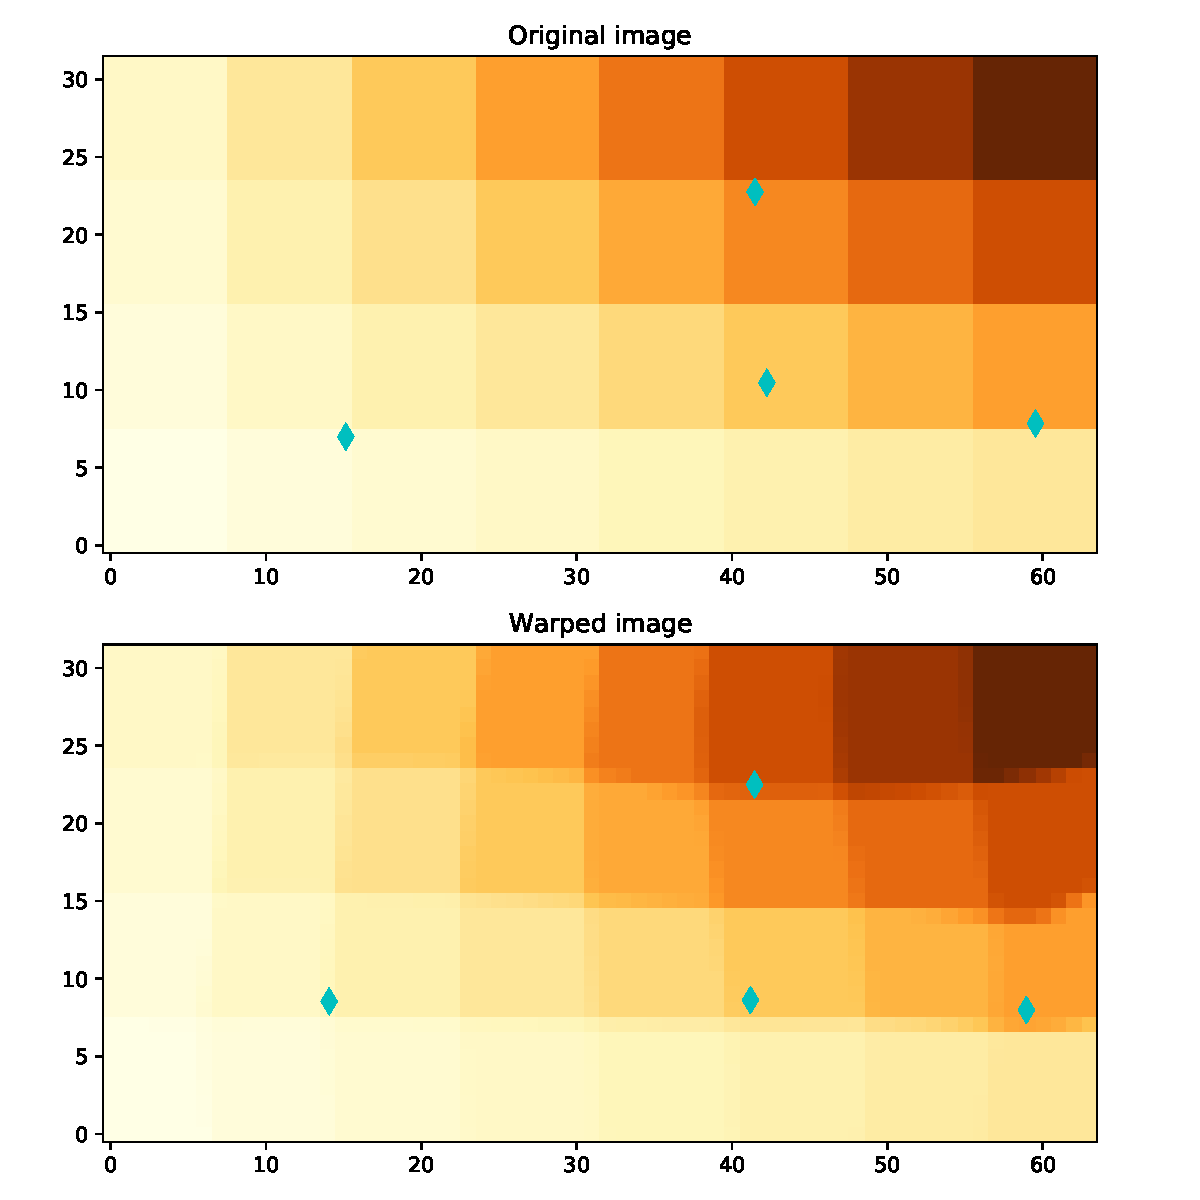
\includegraphics[width=0.9\linewidth]{warp_grid.pdf}
    \caption{
    The effects of \texttt{sparse\_image\_warp} on an image, with
\texttt{num\_landmarks} $=4$, \texttt{max\_warp\_time} $=2$ and
\texttt{max\_warp\_freq} $=2$. The diamonds show the source and destination
landmarks.}%
    \label{fig:warp_grid}
\end{figure}

\section{Learning Framework}
\label{sec:learning_framework}

The training was done using the tensorflow library \cite{tensorflow2015-whitepaper}.

Several training parameters were tweaked during the experiments to maximize the models' performance.
A brief overview of each parameter follows.

\subsection{Learning rate schedule}

\subsubsection{Finding optimal LR values}

% \begin{figure}[t!]
%     \centering
%     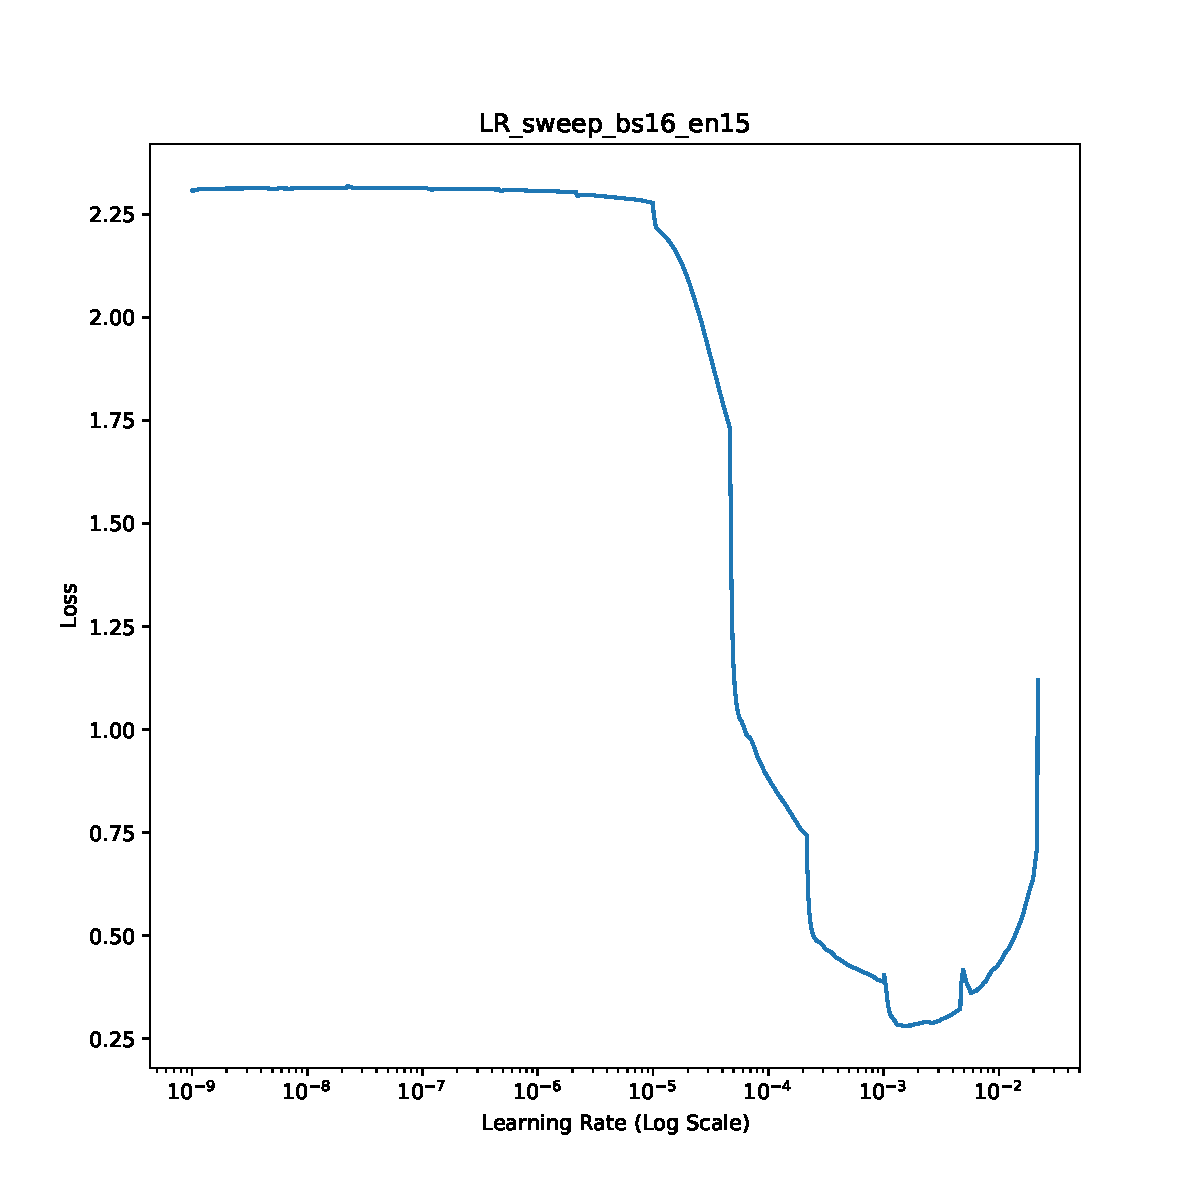
\includegraphics[width=0.9\linewidth]{LR_sweep_bs16_en15.pdf}
%     \caption{LR_sweep_bs16_en15}%
%     \label{fig:LR_sweep_bs16_en15}
% \end{figure}

% https://latexdraw.com/how-to-annotate-an-image-in-latex/
\begin{figure}[t!]
    \centering

    \begin{tikzpicture}

        % \node (image) at (0,0) {
        % \node[anchor=south west] (image) at (0,0) {
        \node[above right] (image) at (0,0) {
            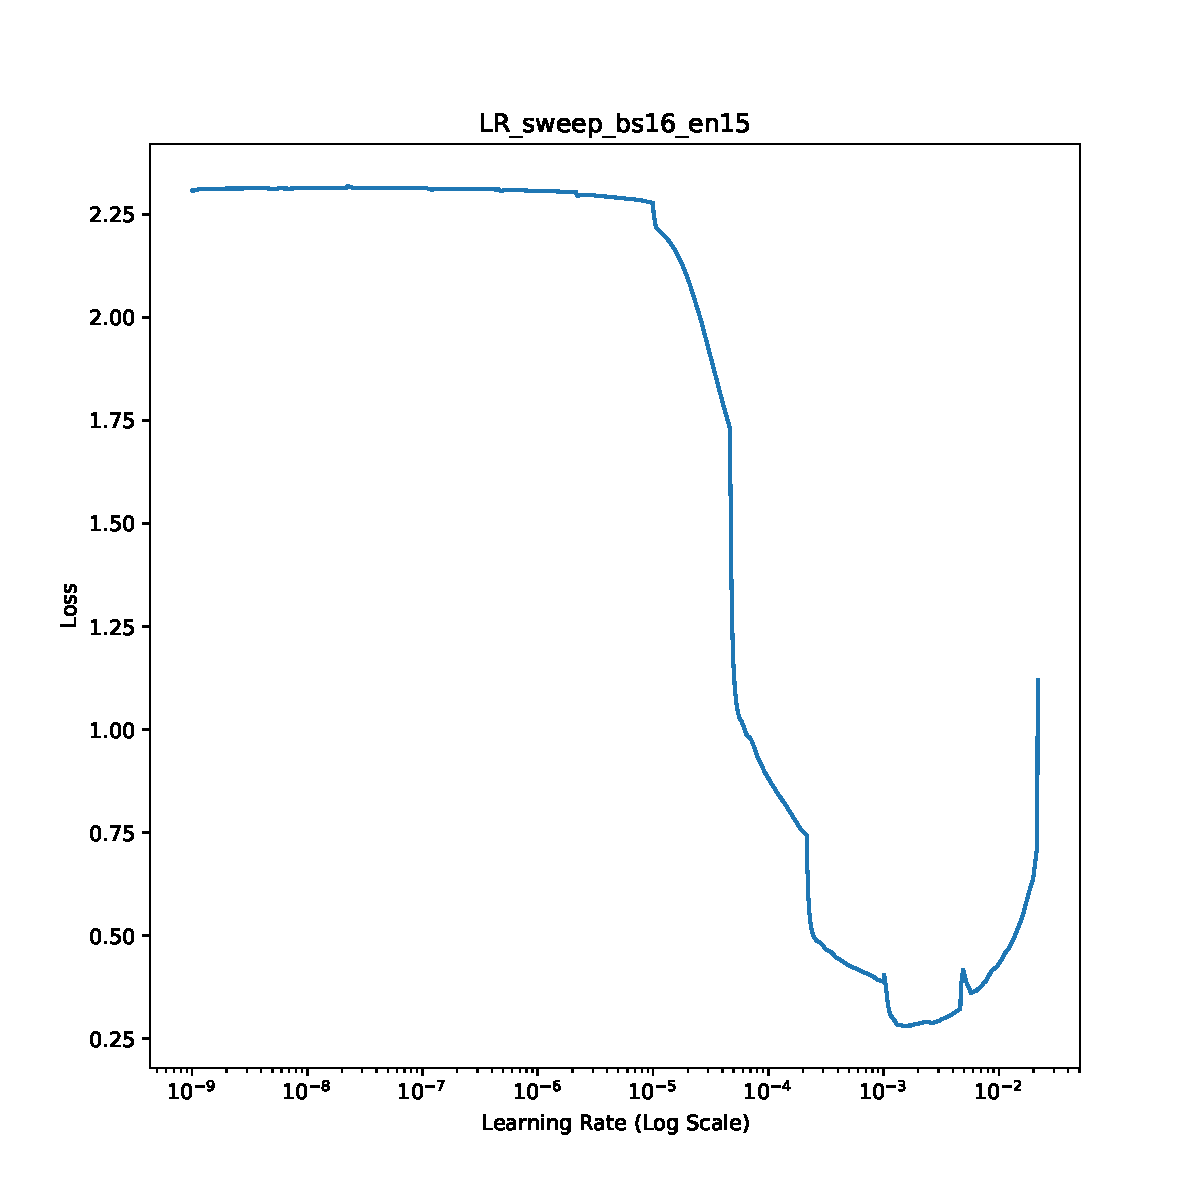
\includegraphics[width=0.9\linewidth]{LR_sweep_bs16_en15.pdf}
        };

        \draw[latex-, very thick,red] (4.3,6.4) -- ++(-1,-1.2)
            % node[left,black,fill=white]{\small Voltage source};
            % node[below left, black, fill=white, text width=2.5cm]{\small The loss starts to drop at $1e-5$};
            node[below, black, fill=white, text width=2.5cm]{\small The loss starts to drop at $1e-5$};

    \end{tikzpicture}

    \caption{LR_sweep_bs16_en15}%
    \label{fig:LR_sweep_bs16_en15}
\end{figure}


\subsubsection{Fixed LR}
\subsubsection{Exp decay LR}
\subsubsection{Cyclic LR}

\subsection{Optimizer}

\subsection{Regularization and Batch Normalization}

\subsection{Early stopping}

Loss, validation, overfitting

Show a plot

Model checkpointing

TensorBoard

\subsection{Hyper-parameter tuning}

Come lo fai

Usare Pool

Ovviamente non su tutte le combinazioni

Pay attention (no pun) to over-representation of the good params.

Epoche/batch, tempo di computazione

\section{Convolutional Neural Network}
\label{sec:convolutional_arch}

\subsection{Architecture}

As a starting benchmark, a standard Convolutional Neural Network was implemented.
Three convolutional modules are instantiated, followed by a dense classifier.
Each convolutional module is composed of the convolutional layer, a batch
normalization layer, a max pooling layer and a dropout layer.
The classifier is composed by three dense layers, the last with softmax
activation and a number of units equal to the number of classes to predict.

\subsection{Model hyper-parameters}

When building the model, aside from the number of classes to predict and the
input shape of the spectrogram, five parameters can be set:
\begin{enumerate}
    \item Number of convolutional filters: deeper layers have to learn more
        filters, as the feature maps decrease in width and height after the
        pooling.
    \item Shape of the convolutional filters:
        both square and rectangular filters were tested.
        A vertical rectangular filters (e.g. (5, 1)) emphasizes the
        relationship between mel coefficients within the same time step
    \item Shape of the pooling window: 
        both square and rectangular windows were tested.
        Again, a rectangular filter allows to push into deeper layers more
        information along the time or frequency axis.
    \item Dropout rates after the convolutional modules.
    \item Width of the dense classifier layers.
\end{enumerate}
The possible values for the hyper-parameters are:
\begin{itemize}
    \item dense\_width = [16, 32, 64, 128]
    \item filters = [10, 20, 32, 64, 128]
    \item dropout = [[0.03, 0.01],  [0.3, 0.1]]
    \item kernel\_size = [[(2,2), (2,2), (2,2)], [(5,1), (3,3), (3,3)]]
    \item pool\_size = [[(2,2), (2,2), (2,2)], [(2,1), (2,2), (2,2)]]
\end{itemize}

% hypa_grid['dataset'] = ['mfcc01' 'aug13' 'mel01' 'aug02' 'mfcc03' 'aug07' 'aug04' 'mel03'
%  'mfcc04' 'mfcc02' 'mel04' 'aug10' 'aug03' 'mel02' 'aug06' 'aug05' 'mela1'
%  'aug09' 'aug08' 'aug12' 'aug11' 'aug14' 'aug15']
% hypa_grid['words'] = ['f1' 'num' 'k1' 'w2' 'f2' 'all' 'dir']

% hypa_grid['batch_size'] = [128  32  64]
% hypa_grid['epoch_num'] = [ 60  15  16  30  59  58  61  31  62 101]
% hypa_grid['lr'] = ['default' '01' '03' '02' '06' '04' '05' 'e1']
% hypa_grid['opt'] = ['adam' 'a1' 'r1']


\section{Transfer Learning Approach}
\label{sec:transfer_learning}

\subsection{Transfer learning}

Transfer learning is a technique where a model developed and trained for a task
is modified slightly and used as a starting point for a different task.
A Convolutional Neural Network can be seen as a feature extractor composed with
a classifier.
The feature extractor is the largest part of the network, consisting in roughly
90\% of the trainable weights.
The idea behind transfer learning is to leverage the knowledge acquired
regarding the first part, extracting meaningful features from an image, and
modifying the latter, re-learning the classifier.
Training these big networks (10-100 millions of parameters) on ImageNet (14
millions of images in 1000 classes) can take from days to over a month even on
supercomputers with dozens of top of the line graphics cards.
Adapting the networks for a new task, on the other hand, is a matter of roughly
half an hour on a single GPU.

As spectrograms can be interpreted as images, starting from an image classifier
makes perfect sense. The two architecture used are Xception 
\cite{chollet2017xception}
and EfficientNet
\cite{tan2020efficientnet}.

\subsubsection{Xception structure}

A standard convolutional layer tries to learn 3D filters, with two spatial
dimensions and one channel dimension.
Such a filter has to simultaneously learn spatial correlations and
cross-channel correlations.
The Inception Hypothesis asserts that it would be easier to learn independently
the cross-channel and spatial correlations.
To do so an Inception module first learns cross-channel correlations with 1x1
convolutions, then learns spatial correlations with standard 3x3 and 5x5
convolutions.
The Xception model pushed this hypothesis to the limit, completely decoupling
the mapping of spatial and cross-channel correlations.

\subsubsection{EfficientNet structure}

Scaling a Convolutional Neural Network can lead to increased performance:
adding more layers, more filters of more convolutional modules can make the
model more accurate. On the other hand, a bigger model means slower training
and higher memory consumption to the point of being infeasible to train.
On top of that, often CNN can be over-parametrized: model compression
techniques can trade little accuracy for a great reduction in model size
\cite{han2016deep}.

The EfficientNet authors carefully examine the scaling of a model to obtain the
optimal parameters of width, depth and resolution, proposing a new compound
scaling method, which uses a single compound coefficient to scale the three
parameters in a coordinated way.
% which use a compound coefficient φ to uniformly scales network width, depth,
% and resolution in a principled way we have also developed a new mobile-size
% baseline, called EfficientNet fix φ = 1, assuming twice more resources
% available, and do a small grid search of α, β, we then fix α, β, γ as
% constants and scale up baseline network with different φ

\subsection{Transfer learning and fine tuning}

The pipeline to train a model using transfer learning is as follows:
\begin{enumerate}
    \item Load a previously trained base model, without the final classifier.
    \item Freeze the base model weights, to avoid destroying the information they
        contain.
    \item Add a classifier on top of the base model.
    \item Train the classifier, using a reasonably high learning rate.
    \item Un-freeze the base model weights.
    \item Train the model again, with a very small learning rate, to fine tune
        the feature extractor to the current dataset.
\end{enumerate}

The first four steps are the transfer learning part, followed by the fine
tuning steps five and six.

\subsection{Model building and hyper-parameters}

The inputs to the pre-trained Xception and EfficientNet models have to be
square images with three channels.
To appropriatley shape the input data, three square spectrograms were stacked
along the depth dimension.
On top of that, to obtain square inputs, two rectangular spectrograms were
concatenated horizontally (e.g. two $\left( 128, 64 \right)$ spectrogams are
composed into one $\left( 128, 128 \right)$), before being stacked.
The inputs also need to be normalized, which can be easily done with a
Normalization layer provided by tensorflow.
It is to note that the inputs should be of higher resolution (e.g. $\left( 299,
299, 3 \right)$ for Xception), whereas the spectrograms used were of size
$\left( 128, 128, 3 \right)$, so some loss of performance can be expected.
The classifier built is composed by a GlobalAveragePooling2D layer, which
averages the values in each feature extracted, followed by some dense layers
(according to the hyper-parameters selected) and finally a softmax layer to
compute the predictions.

When building the model, aside from the number of classes to predict and the
input shape of the spectrograms, two parameters can be set:
\begin{enumerate}
    \item Dropout rate after the GlobalAveragePooling2D layer.
    \item Dense width and number of the dense layers in the classifier.
\end{enumerate}
The possible values for the hyper-parameters are:
\begin{itemize}
    \item dropout\_types = [0.2, 0.1, 0]
    \item dense\_width\_types = [[4, 0], [16, 16], [0, 0], [64, 64]]
\end{itemize}
Where a value of $0$ means that the layer is skipped.

\section{Attention Model}
\label{sec:attention_model}

\subsection{Attention architecture}

The key idea behind the Attention mechanism is the assumption that not all of
the data that is available carries the same amount of information.
% Indeed, when processing a large amount of information we focus on few relevant details.
The attention mechanism allows to focus on few relevant details when presented
with large amount of data.
This approach was used effectively in the field of Neural Machine Translation
by Bahdanau \cite{bahdanau2016neural} and Luong \cite{luong2015effective}, and
to produce image captions with the Show, Attend and Tell approach
\cite{xu2016show}.

In the paper by Douglas et al. \cite{2018arXiv180808929C}, the attention
mechanism is used for speech command recognition.
The ouput shapes of each layers are reported to track along which axis the dot
multiplications are done.
As a first step, the mel spectrogram
(shape [spec\_len, nMel])
is computed from the input audio
(shape [raw\_len]).
A 2D convolution is performed, only along the time axis to extract local
correlations in the spectrogram
(shape [spec\_len, nMel, n\_filters]).
A final 2D convolution, with just one filter, condenses the information back to a 2D image
(shape [spec\_len, nMel, 1])
and the last dimension is squeezed away
(shape [spec\_len, nMel]).
Two bidirectional \cite{Schuster1997BidirectionalRN} long short-term memory
\cite{lstm} units are used to capture forward and backward long term
dependencies in the spectrogram
(shape [spec\_len, LSTM\_units*2]).
A LSTM layer reads the input sequence from the first sample to the last. The
bidirectional version reads the sequence both forward, producing the forward
hidden states, and backward, resulting in the sequence of backward hidden
states.
Now the attention mechanism is applied: one of the LSTM output vector is
selected (the choice is not crucial because the vectors should contain
information about long term dependencies) and a dense layer is used to extract
a query vector
(shape [LSTM\_units*2]).
The query vector is used to compute the attention scores, by computing the dot
product between all the LSTM outputs and the query vector along the
\textit{second} axis of the LSTM outputs, that are converted with a softmax
layer in attention weights
(shape [spec\_len]).
These weights are multiplied with the output of the LSTM along the
\textit{first} axis of the LSTM outputs to compute a weighted average of the
LSTM vectors
(shape [LSTM\_units*2]),
which is then fed into a dense classifier
(shape [nClasses]).
In this way, the output vector of the LSTM is not just the final hidden state,
but it is a function of all the hidden states, where the most important states
are given more relevance, according to the attention weights.

\subsection{Query style}

Two additional methods to compute the query were developed and tested.
In the first method, from the output of the second LSTM layer, a CNN was used
to extract the query, using several convolutional modules.
In the second method, the query was directly computed from the input
spectrogram, using a CNN.
A third query style tested is regarding the choice of LSTM output vector to
pick to compute the query: instead of the last, the central vector was chosen.

TODO: un grafichetto sarebbe bellissimo

\subsection{AreaNet}

Dream a dream

\subsection{Model building and hyper-parameters}

When building the model, aside from the number of classes to predict and the
input shape of the spectrograms, six parameters can be set:
\begin{enumerate}
    \item Number of convolutional filters in the convolutional modules.
    \item Dropout rate after the convolutional modules.
    \item Shape of the convolutional filters:
        both square and rectangular filters were tested.
        A vertical rectangular filters (e.g. (5, 1)) emphasizes the
        relationship between mel coefficients within the same time step
    \item Number of LSTM units.
    \item Query style: either a single output vector from the LSTM or the
        result of a convolutional operation, that takes as input the original
        spectrogam or the vectors produced by the LSTM.
    \item Width of the dense classifier layers.
\end{enumerate}
The possible values for the hyper-parameters are:
\begin{itemize}
    \item conv\_size = [[10, 0, 1], [10, 10, 1]]
    \item dropout = {0.2, 0}
    \item kernel\_size = [[(5,1), (5,1), (5,1)], [(3,3), (3,3), (3,3)]]
    \item lstm\_units = [[64, 64], [64, 0]]
    \item query\_style = ["dense01", "dense02", "conv01", "conv02", "conv03"]
    % \item query\_style = [\texttt{dense01}, \texttt{dense02},
    % \texttt{conv01}, \texttt{conv02}, \texttt{conv03}]
    \item dense\_width = [32, 64]
\end{itemize}



% !TEX root = report.tex

\section{Results}
\label{sec:results}
% Dazzling numerical results

\subsection{Performance measure}

% \subsubsection{F-Score}

The F-Score is a metric that combines the values of precision and recall to
provide an estimate of the quality of the predictions made on a test dataset.
Precision is the fraction of relevant data among the selected instances, the
number of true positives over all the samples selected (a high precision score
means that there are few false positives).
% MAYBE how confident you are that a selected is really in that class.
Recall is the fraction of selected instances among all the relevant samples,
the number of true positives over all the true samples (a high recall score
means that there are few false negatives). The F-Score is obtained as the
harmonic mean of precision and recall.

% Confusion matrix
Another tool used to visually show the performance of a model
is the confusion matrix, that is closely related to the F-Score.
The predicted labels are listed on the x-axis,
the real labels are listed on the y-axis.
% On the x-axis the predicted labels are listed,
% on the y-axis the real labels are listed.
The confusion matrix contains
the number of occurences
for each combination of predicted/real labels.
The main diagonal contains the correctly identified samples.
Along the rows there are the false negatives for a label,
and along the columns there are the false positives for a label.

% \subsubsection{Graphs}

Throughout this section, several groups of graphs will be shown, that present
at once the F-score value for combinations of up to four hyper-parameters.
For example, say there is a graph 
with title 
``paramA: valueA, paramB: [valuesB]
grouped by paramC: [valuesC]
grouped by paramD: [valuesD]''.
This graph is part of a group of graphs, where the value of the first parameter
(valueA) is fixed for each sub-graph.
The other three parameters vary within the sub-graph:
% each packet of columns shows the variation of the parameter B,
% whose values are shown in the legend.
within each group of column the parameter B is changing,
whose values are shown in the legend.
% The groups of columns show the variation of the parameter C,
% whose values are shown as labels of the x axis.
% Each super group of columns show the variation of the parameter D,
% whose values are shown between parenthesis as labels of the x axis.
The other two parameters vary for each group of columns:
the values are indicated in the label of the x axis as ``valueC (valueD)''.
The other hyper-parameters are averaged for each column.
% , within reason:
% Average the others within reason (eg only one type of task).
The height of the column shows the mean F-score value for that
combination of parameters,
the black line indicates the min/max values of F-score and the
blue line tells the standard deviation around the mean.

\subsection{Hyper-parameter analysis: CNN}

% \subsection{Hyper-parameter analysis}
% Hypa comparison
% First specific hypas

A total of $5064$
% TODO
experiment were performed for the convolutional architecture.

\subsubsection{Model parameters performance comparison}

The effects of tweaking the parameters of the model structure are shown in
\fig{fig:cnn_comparison_kernel_filter_dense_pool}.
The graph sums up the F-Score values for variation of
a)
the number of convolutional filters learned,
b)
the shape of the filters ($01$ for square kernel sizes, $02$ for a vertical
filter followed by two square filters),
c)
the shape of the pooling window ($01$ for square, $02$ for a rectangular
window followed by two square ones)
and
d)
the number of units in the dense classifier.
% clear see kernel
% clear see dense
% pool vague
% filter useless
% Fscore__kernel_size__filters__dense_width__pool_size.png
Several insights can be extrapolated, in order of clarity:
\begin{itemize}
    \item The vertical kernel helps extract information along the frequency axis,
        and provides a clear increase in performance.
    \item A larger dense classifier leads to better performance,
        that saturates at $64$, and further increase does not help.
    \item A high number of filter is not needed to achieve a good performance,
        any value larger than $10$ performed equally well, from $20$ to $128$.
    \item Square pool windows perform slightly better than the rectangular ones.
\end{itemize}

% TODO: on what is averaged

\begin{figure*}[h!]
    \centering
    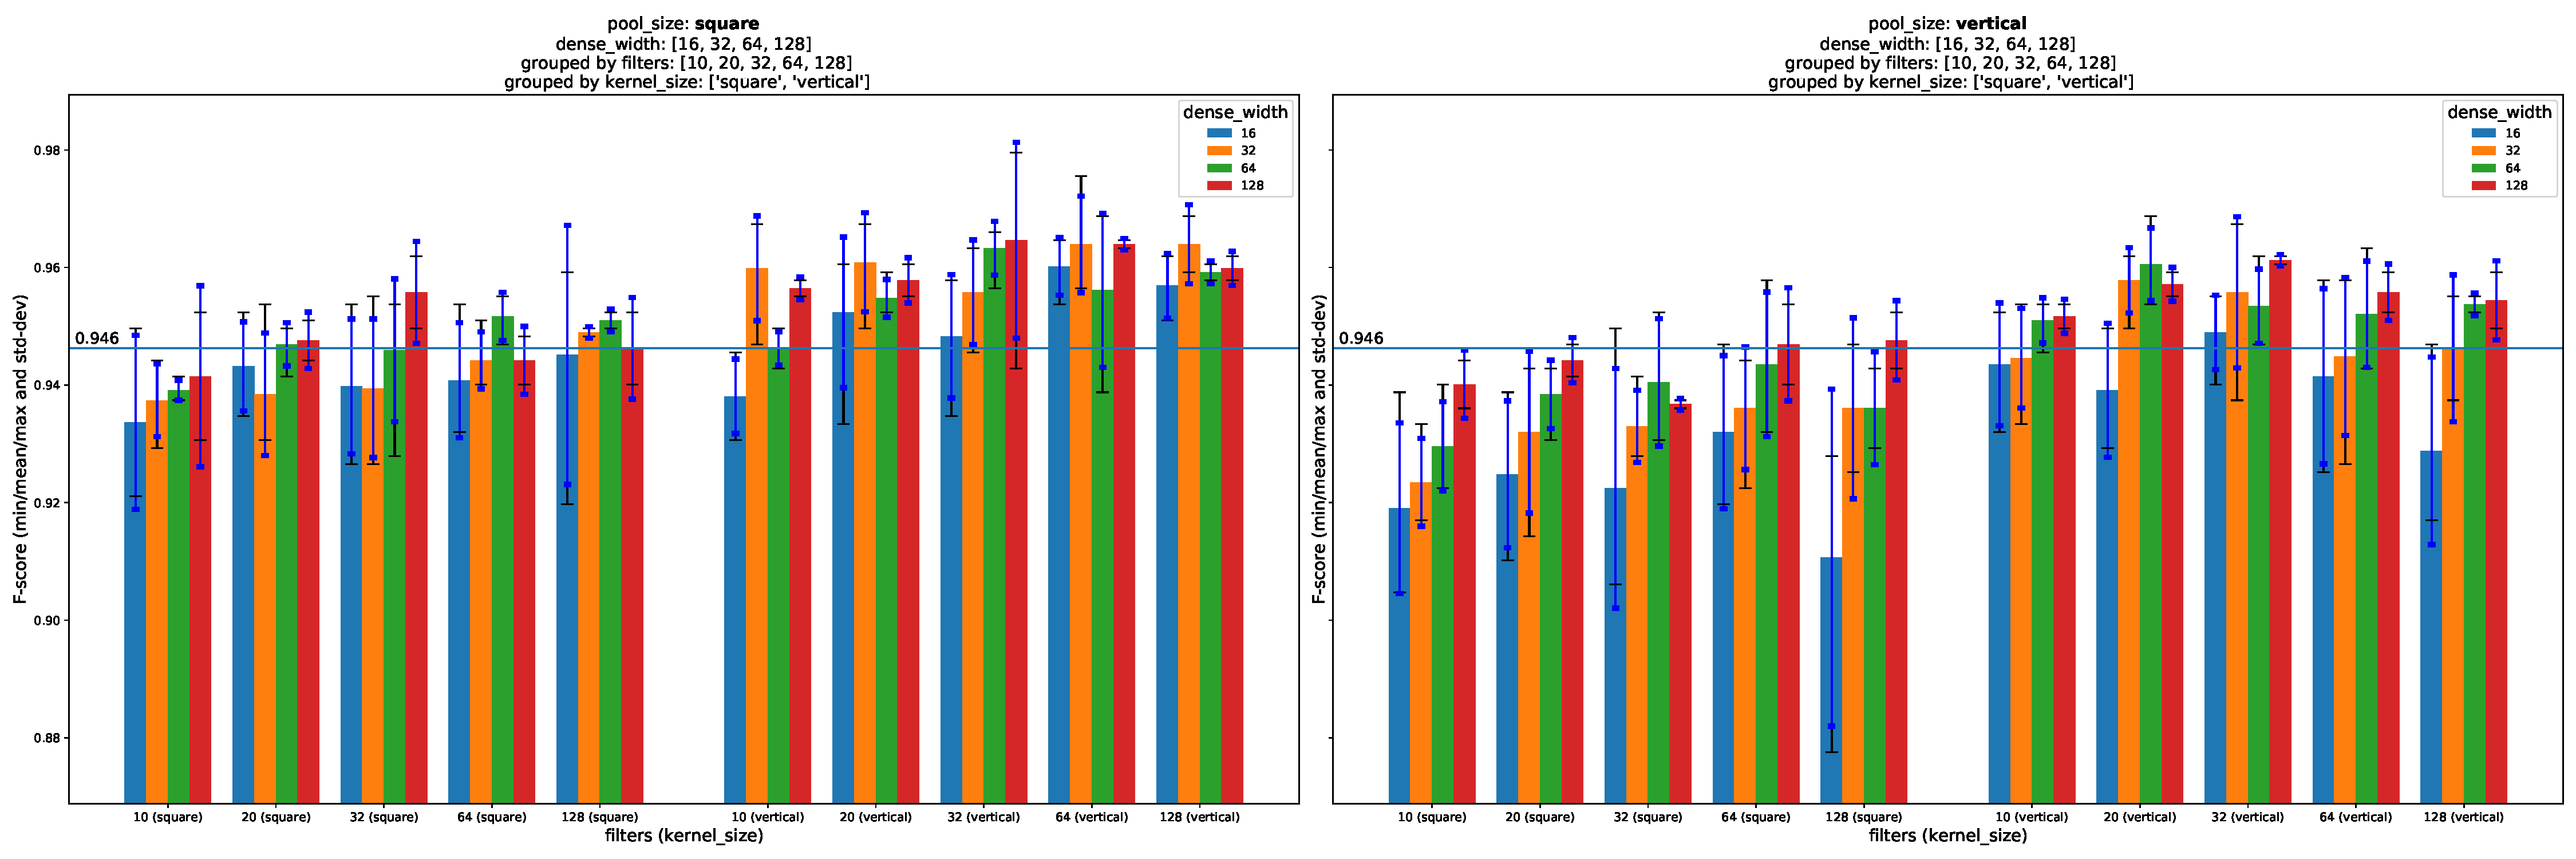
\includegraphics[width=0.9\linewidth]{Fscore_CNN_kernel_size__filters__dense_width__pool_size.pdf}
    \caption{Comparison CNN model}%
    \label{fig:cnn_comparison_kernel_filter_dense_pool}
\end{figure*}

\subsubsection{Training parameters performance comparison}

\fig{fig:cnn_comparison_epoch_lr_dataset} shows F-Score values for
variation of
the dataset used (MFCC spectrogams, mel sectrograms, agumented mel spectrogams)
and the learning rate used (fixed or with exponential decay).
Two main conclusions can be reached:
\begin{itemize}
    \item 
        Mel Frequency Cepstral Coefficients are clearly outperformed by mel
        spectrograms, as expected, considering that the MFCC are built to be composed
        by uncorrelated vectors, so interpreting the input as an image is not
        recommended.
        The benefit of augmentation are less clear, more details are provided
        in \secref{sec:augmentation_performance} and
        \tab{tab:augmentation_comparison_performance}.
    \item 
        The first three packets of columns correspond to fixed learning rate values,
        while the last three correspond to an exponential decay schedule.
        An increase in performance is achieved with the exponential schedules.
\end{itemize}

\begin{figure*}[h!]
    \centering
    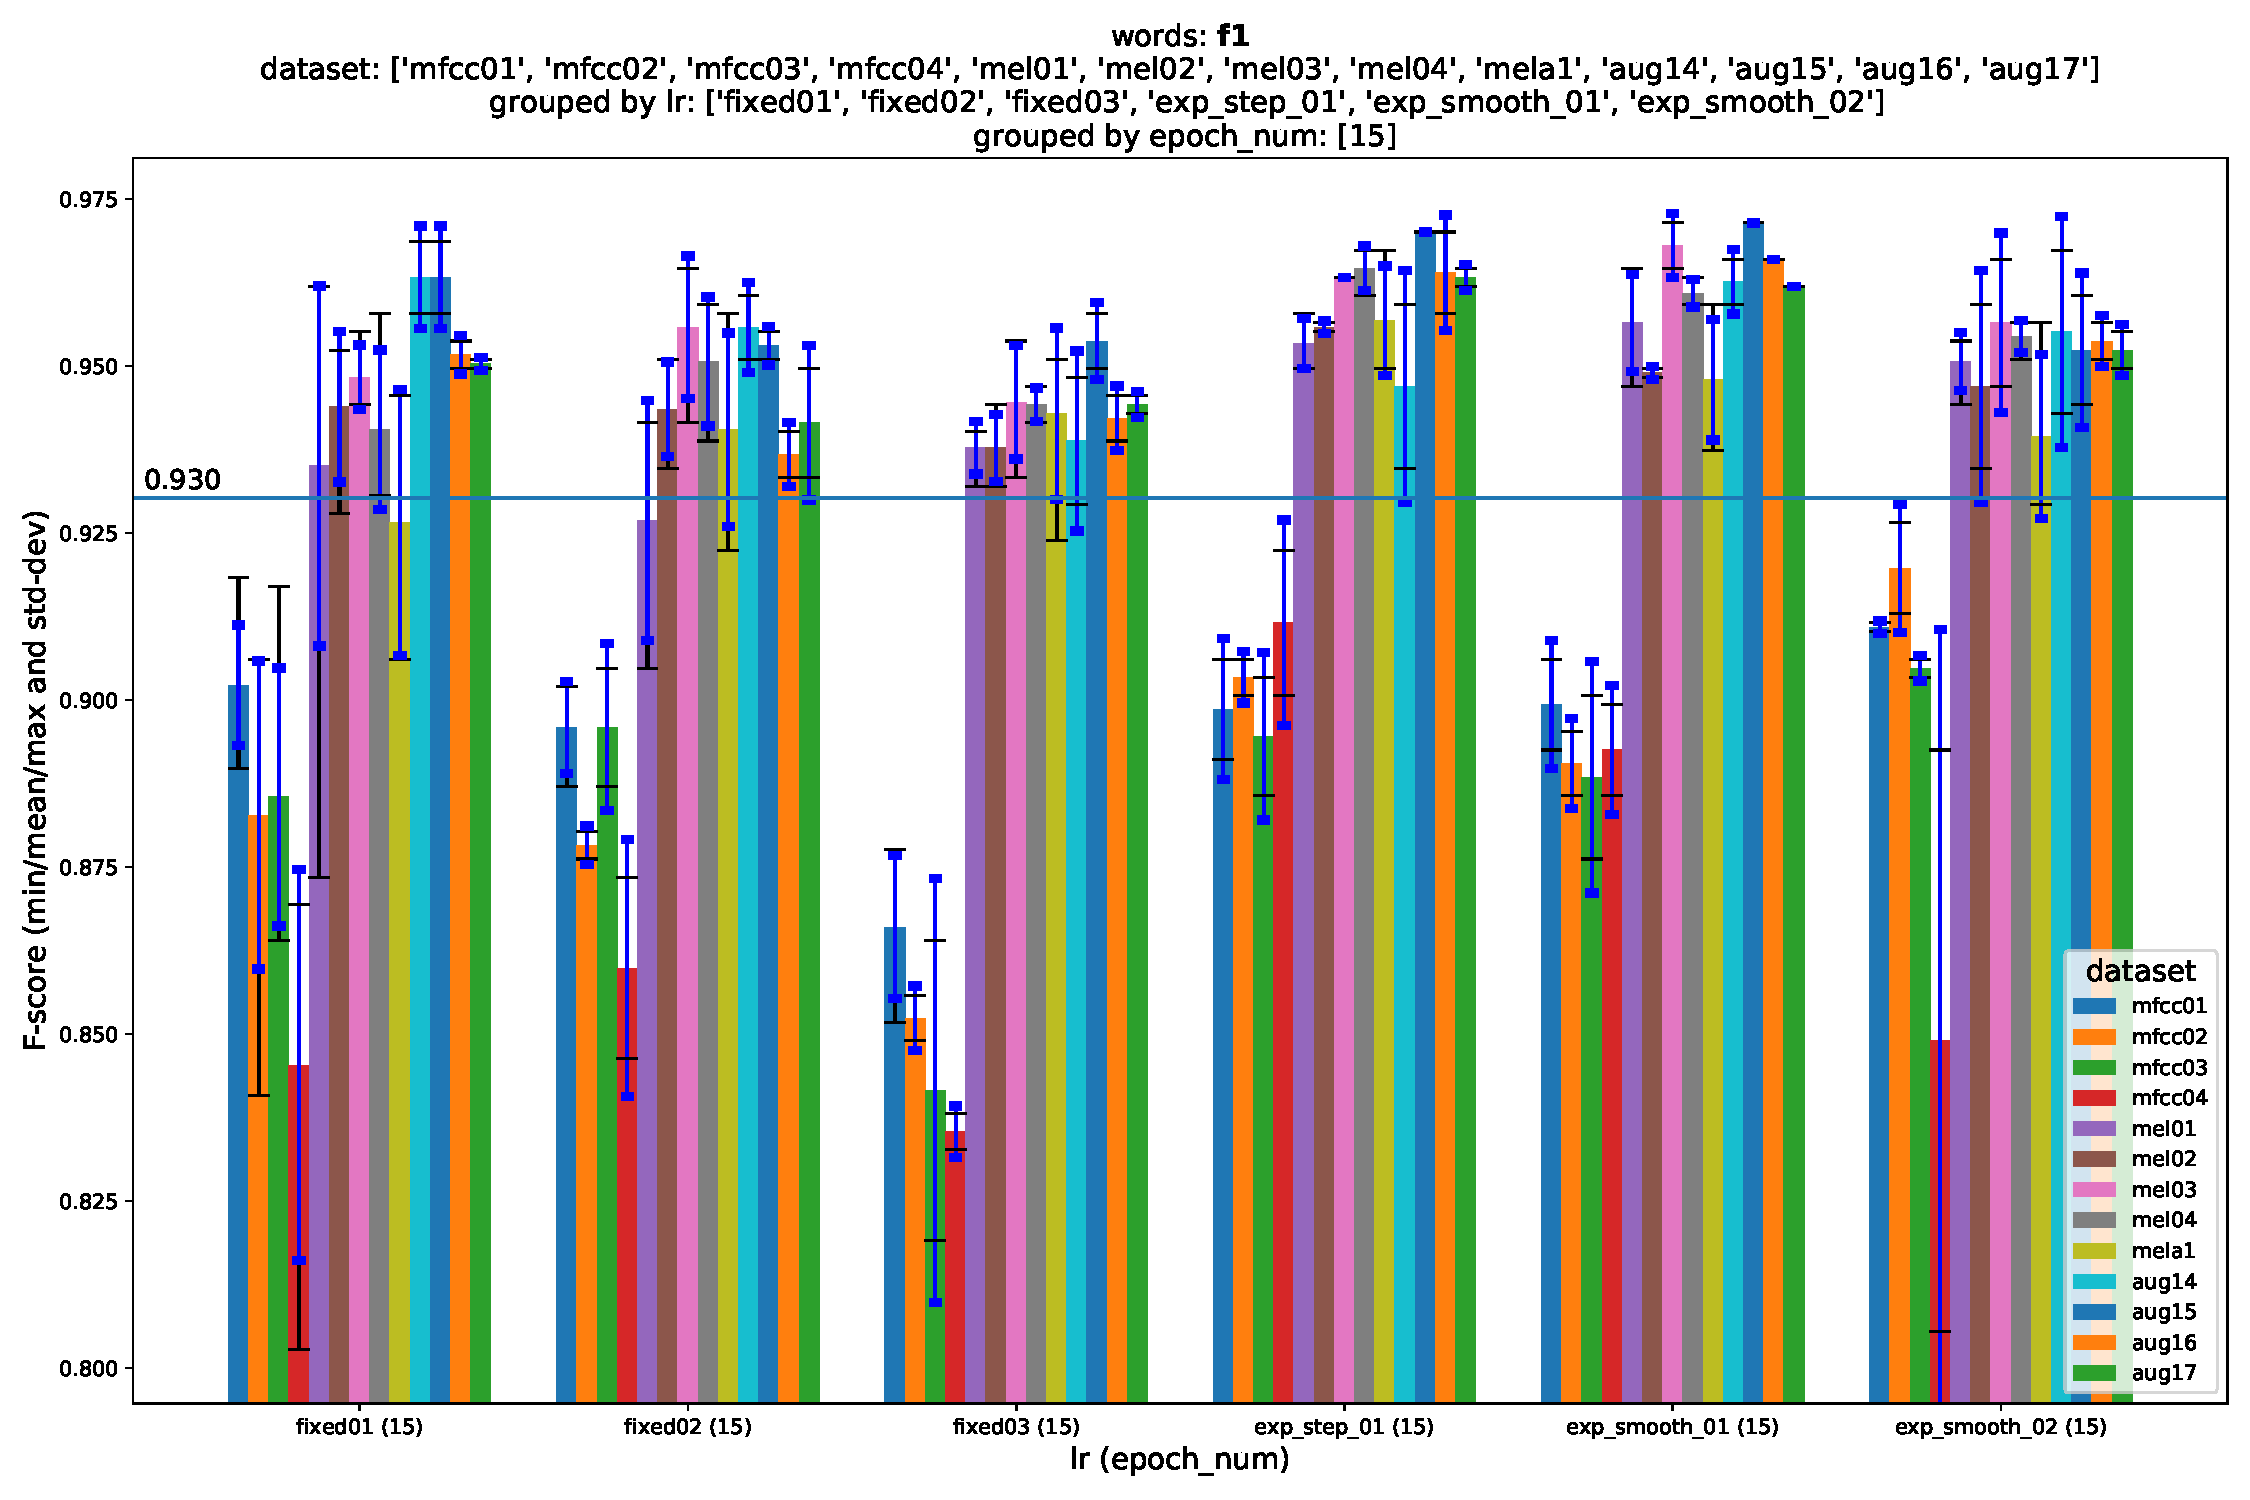
\includegraphics[width=0.9\linewidth]{Fscore_CNN_epoch_num__lr__dataset__words.pdf}
    \caption{Comparison CNN}%
    \label{fig:cnn_comparison_epoch_lr_dataset}
\end{figure*}

\subsection{Hyper-parameter analysis: Transfer learning}

A total of $144$
% TODO
experiment were performed for the transfer learning approach.

% TODO: on what are you averaging

\subsubsection{Model and training parameters performance comparison}

\fig{fig:tra_comparison_batch_epoch_dense} shows the effects of tuning
a)
the number of training epochs
b)
the number of samples per batch
c)
the shape of the final classifier built on top of the Xception model.
% Fscore__batch_size__epoch_num__dense_width__words.png
Using a combination of $[40, 20]$ epochs and $[16, 16]$ as batch sizes seems to
achieve the best performance, while the shape of the classifier does not
influence the training.

% Fscore_TRA_batch_size__epoch_num__dense_width__words.pdf

\begin{figure}[h!]
    \centering
    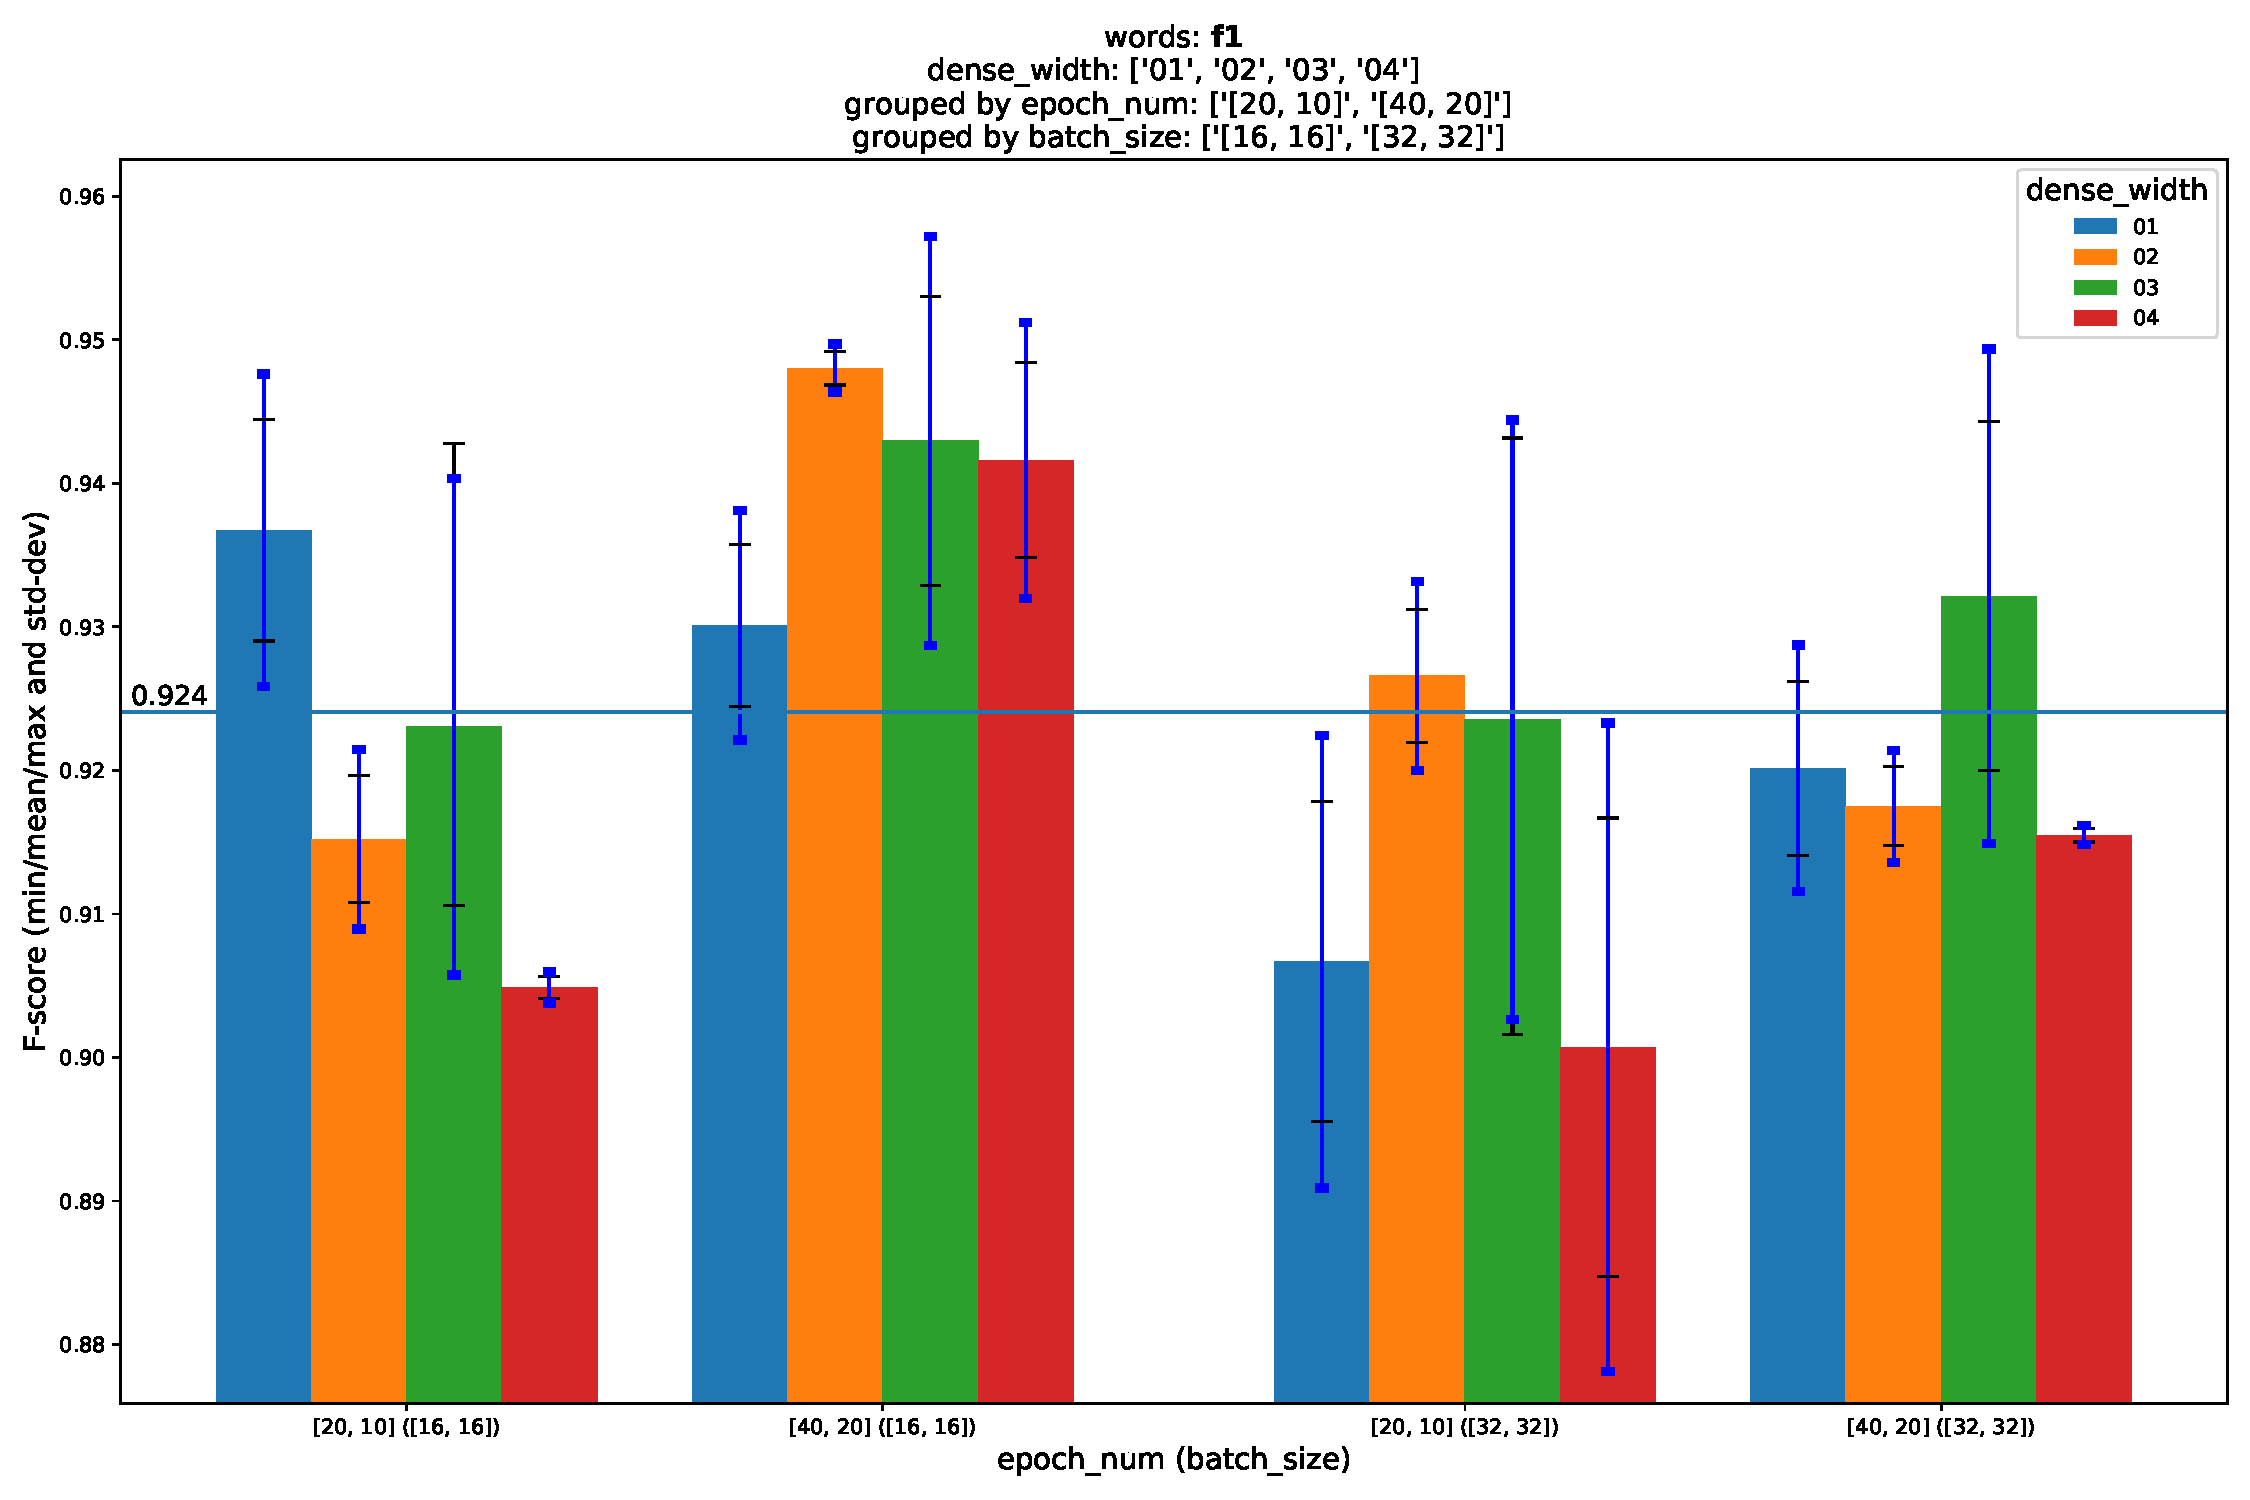
\includegraphics[width=0.8\linewidth]{Fscore_TRA_batch_size__epoch_num__dense_width__words.pdf}
    \caption{TRA comparison batch epoch dense}%
    \label{fig:tra_comparison_batch_epoch_dense}
\end{figure}

\subsubsection{Dataset performance comparison}

\fig{fig:tra_comparison_dataset}

% TODO: what are you averaging?

The different ways used to stack the spectrograms to obtain a 3-channels image
are compared in \fig{fig:tra_comparison_dataset}.
Stacking 128x128 mel spectrograms works quite well, as expected.
Similarly, stacking three mel spectrograms obtained by composing two 128x64
spectrograms each, can lead to similar results.
The MFCC spectrograms do not work as well, just as seen with the small
convolutional networks.
All these images had uniform structure across the depth dimension, as they were
obtained by stacking spectrograms with the same shape and type.
However, reasonably good results are also obtained by stacking spectrograms of
different kinds: both stacking 2 mel and 1 MFCC and stacking 1 mel, 1 MFCC and
1 composed.
In these last two types, there is little cross-channel correlation.
Considering that the base model used is Xception, that learns independently the
spatial and cross-channel correlations, it makes sense that the results are
decent, as the model learns to exploit the spatial correlations, but some
performance is lost as there is no information to be extracted by the
cross-channel correlations between different types of spectrograms.

\begin{figure}[h!]
    \centering
    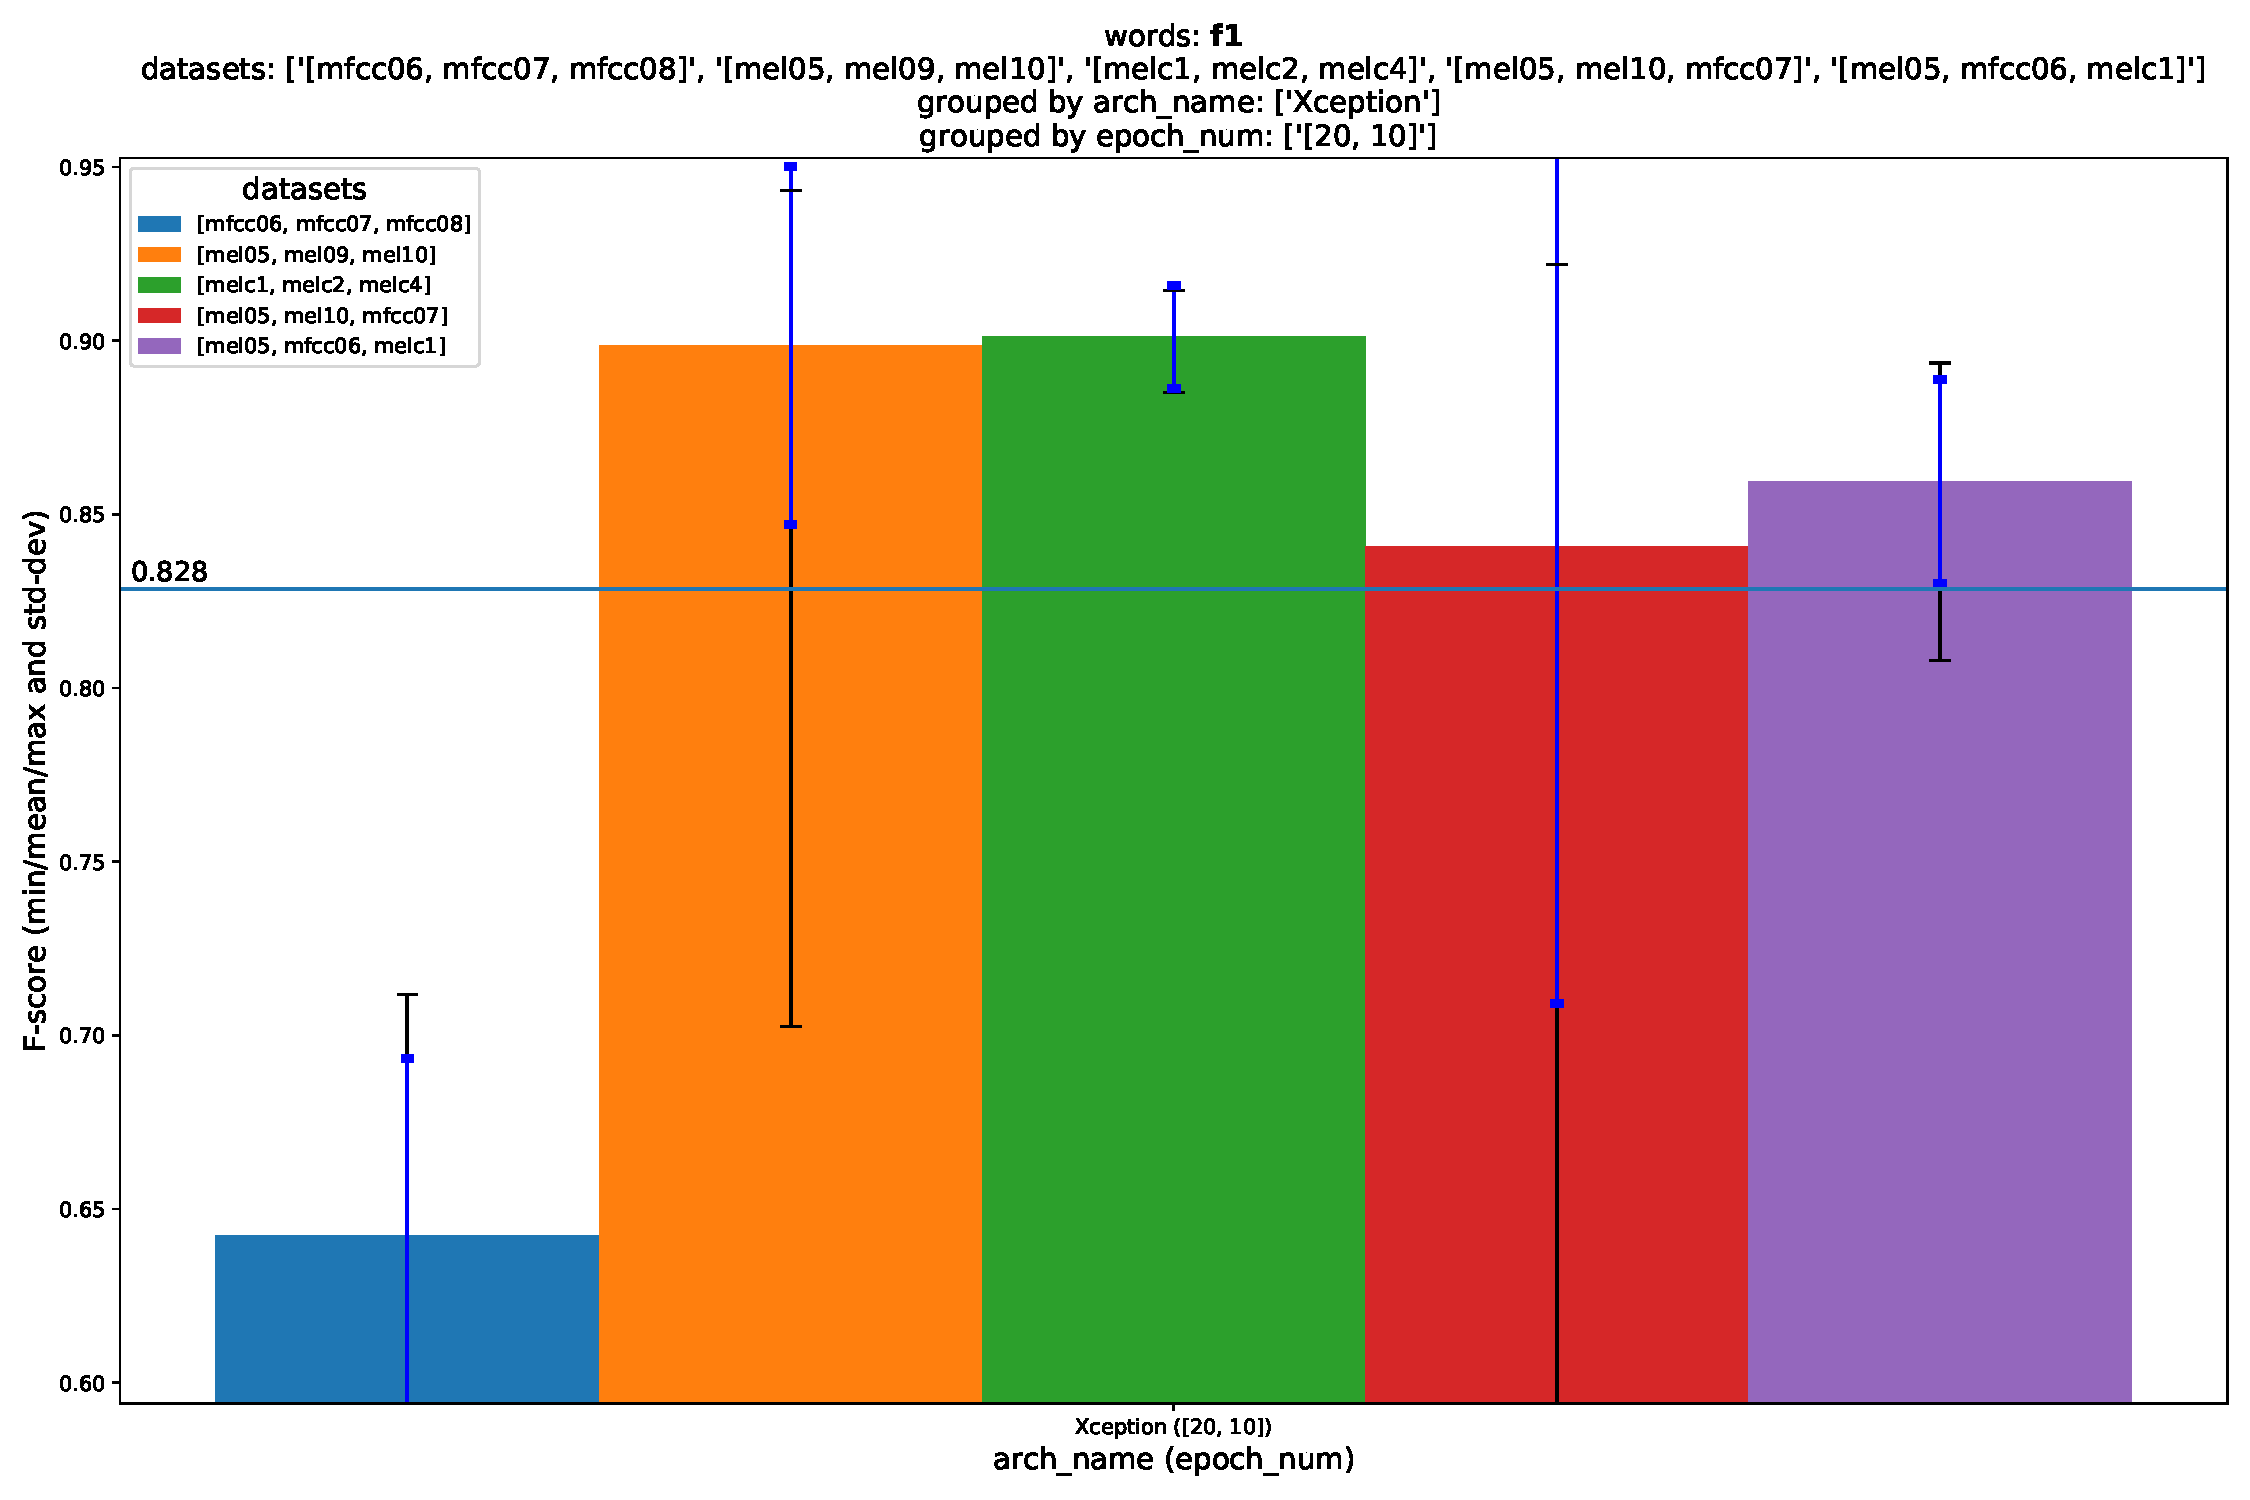
\includegraphics[width=0.8\linewidth]{Fscore_TRA_dataset_comparison.pdf}
    \caption{Dataset TRA comparison}%
    \label{fig:tra_comparison_dataset}
\end{figure}

\subsubsection{Architecture performance comparison}


\fig{fig:tra_comparison_arch} shows the performances of different base models:
The best model architectures are DenseNet121 and EfficientNetB7.
It is worth noting that the latter is a far larger network, as DenseNet121 only
has 7M parameters compared to the 66M of EfficientNetB7.
EfficientNetB4 also achieves very good results, using only 19M parameters,
outperformimg by a little Xception, with 22.8M parameters.
EfficientNetB0, with 5.3M parameters, cannot reach the same results.

% TODO: EfficientNet exactly like in the paper the nice curve precision vs number params

% 7M DenseNet121
% 22.8M Xception
% 5.3M B0
% 19M B4
% 66M B7

\begin{figure}[h!]
    \centering
    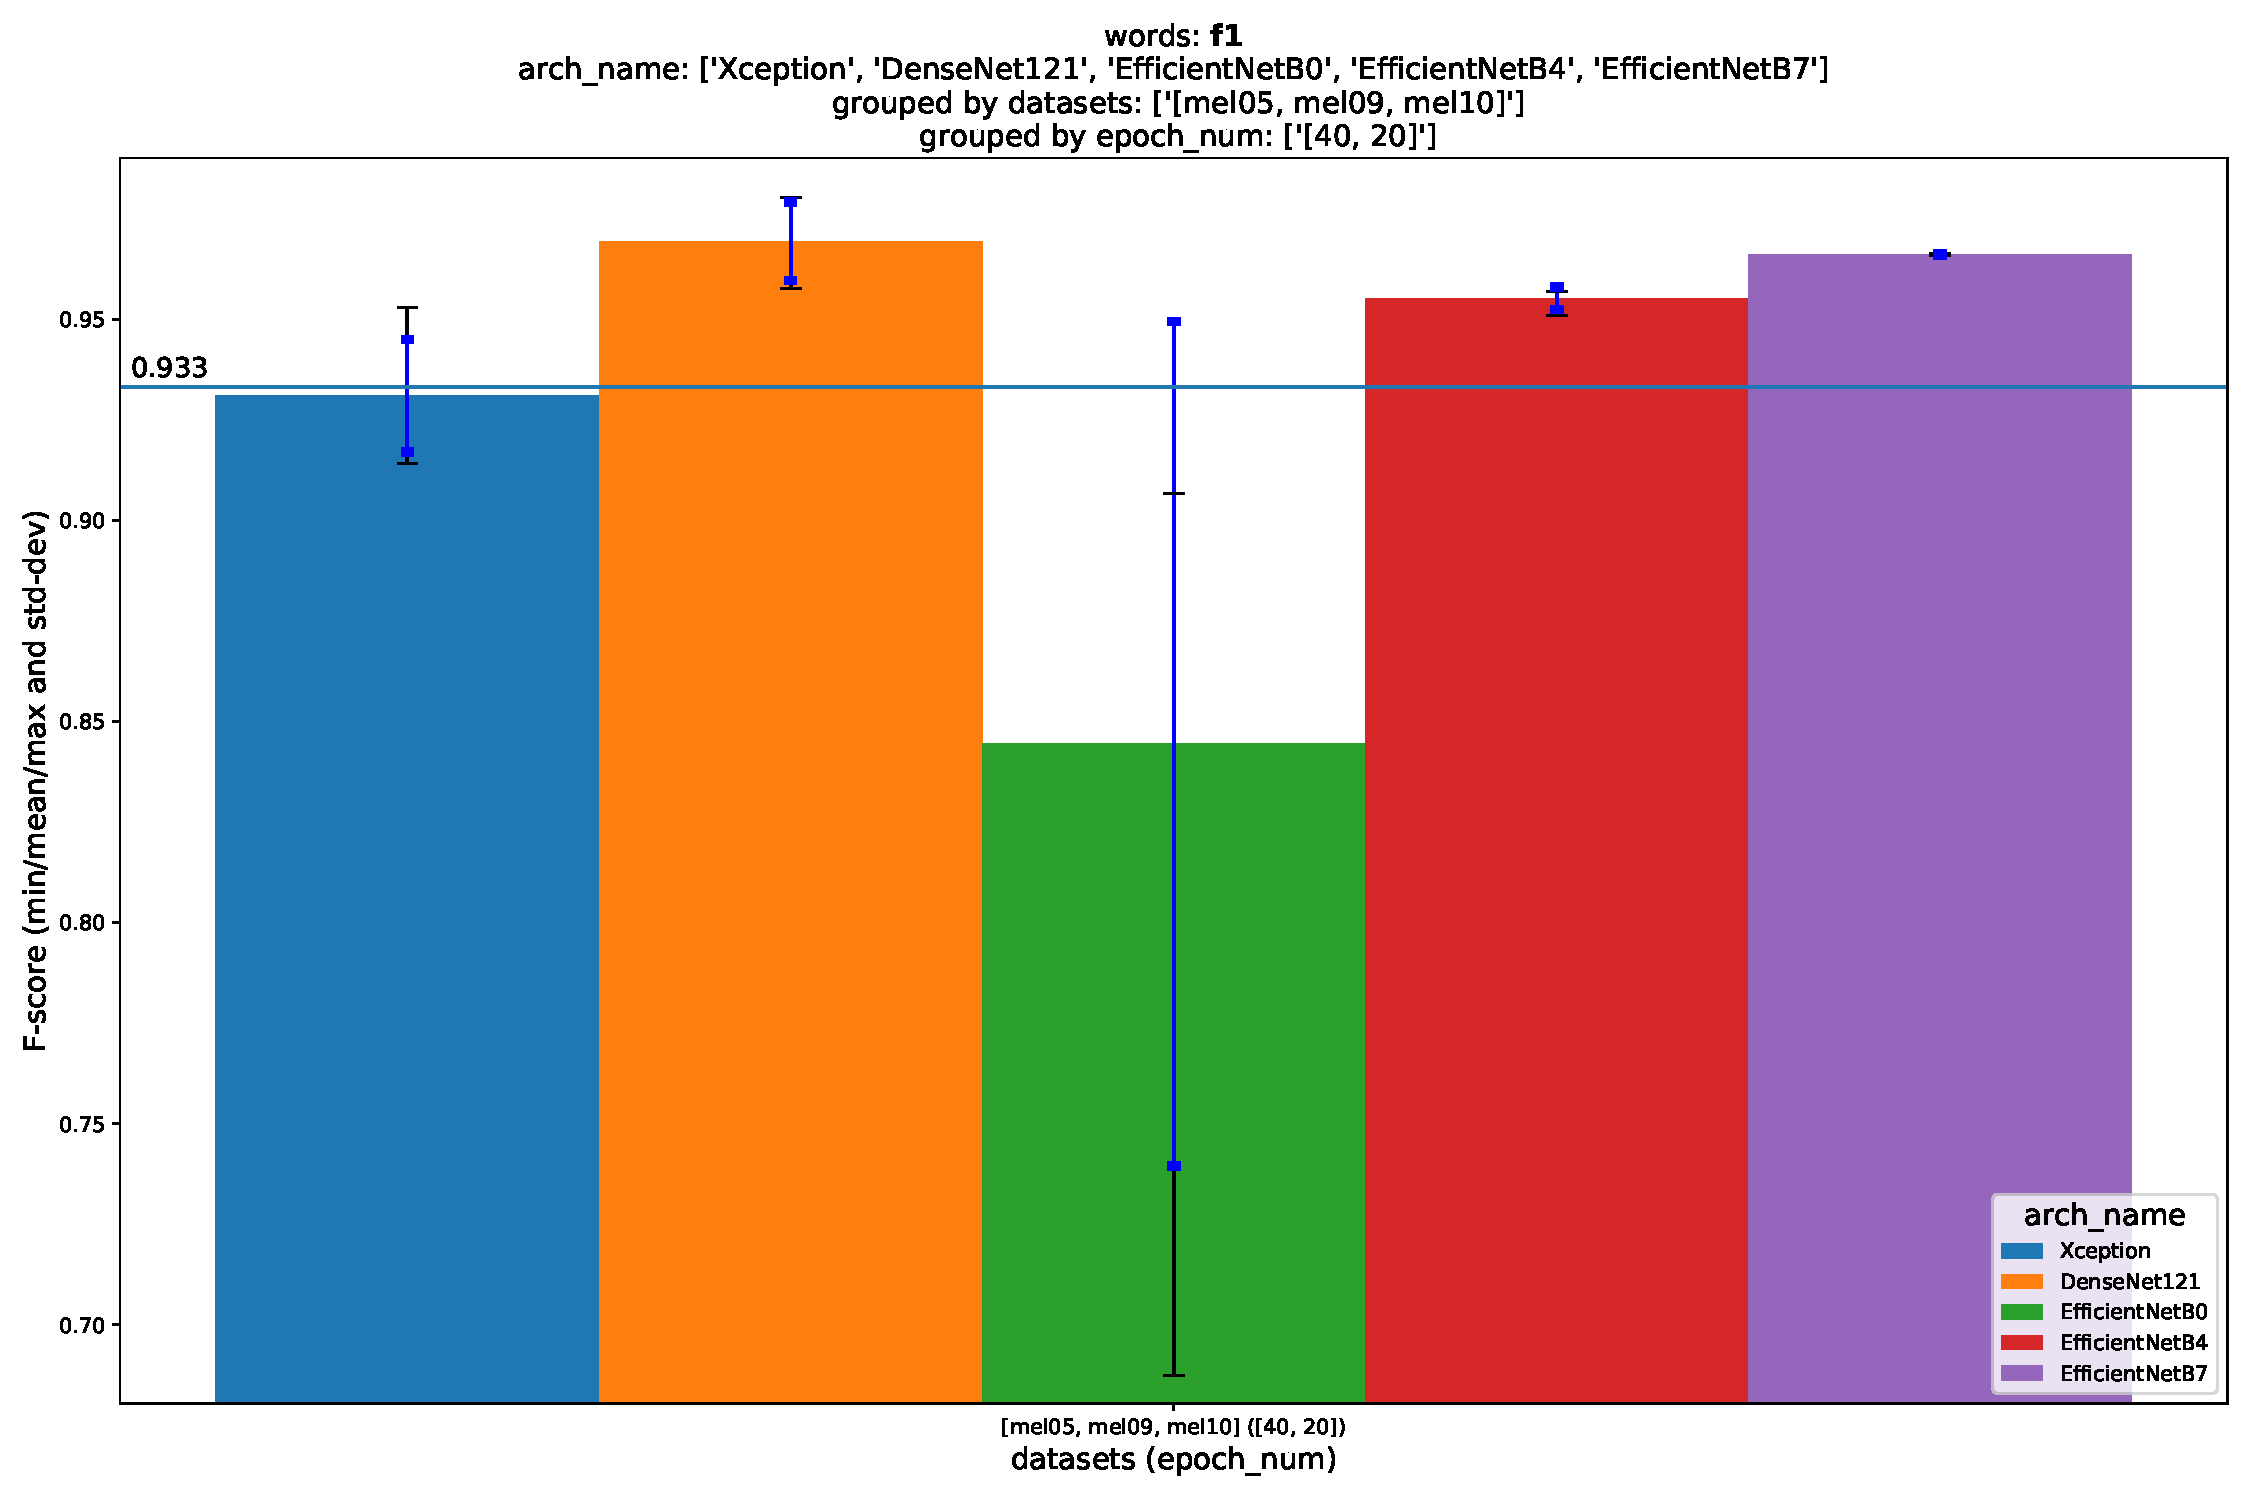
\includegraphics[width=0.8\linewidth]{Fscore_TRA_arch_comparison.pdf}
    \caption{Architecture TRA comparison}%
    \label{fig:tra_comparison_arch}
\end{figure}

\subsection{Hyper-parameter analysis: Attention}

A total of $1688$
% TODO
experiment were performed for the LSTM+attention model.

\subsubsection{Model parameters performance comparison}

\fig{fig:att_dropout_conv_query_dense} shows F-score values for 
variation of 
a)
the width of the dense classifier ($32$ or $64$),
b)
the dropout rate
after the initial convolutional layers
($0.2$ or $0$),
c)
the number of initial convolutional layers ($1$ or $2$)
and
d)
the query style ($01$ and $05$ pick a single LSTM vector to compute the scores,
$02$ and $03$ use convolutional layers connected to the LSTM outputs to extract
the scores and $04$  uses convolutional layers connected to the spectrograms).
The results are very close but two conclusions can be tentatively reached:

\begin{itemize}
    \item The query type does not influence the results: within each packet of
        columns the values are very close to each other, within one standard
        deviation.
    \item The combination of dense 02 ($64$ units), conv 01 ($1$ layer) and
        dropout 01 ($0.2$) seems to be consistently better than the average.
        The best values might be found with other combinations of parameters,
        but those combinations are less robust, as indicated by the higher
        standard deviation, and the quality of the model is less assured when
        training that combination for new datasets.
\end{itemize}

\begin{figure*}[t!]
    \centering
    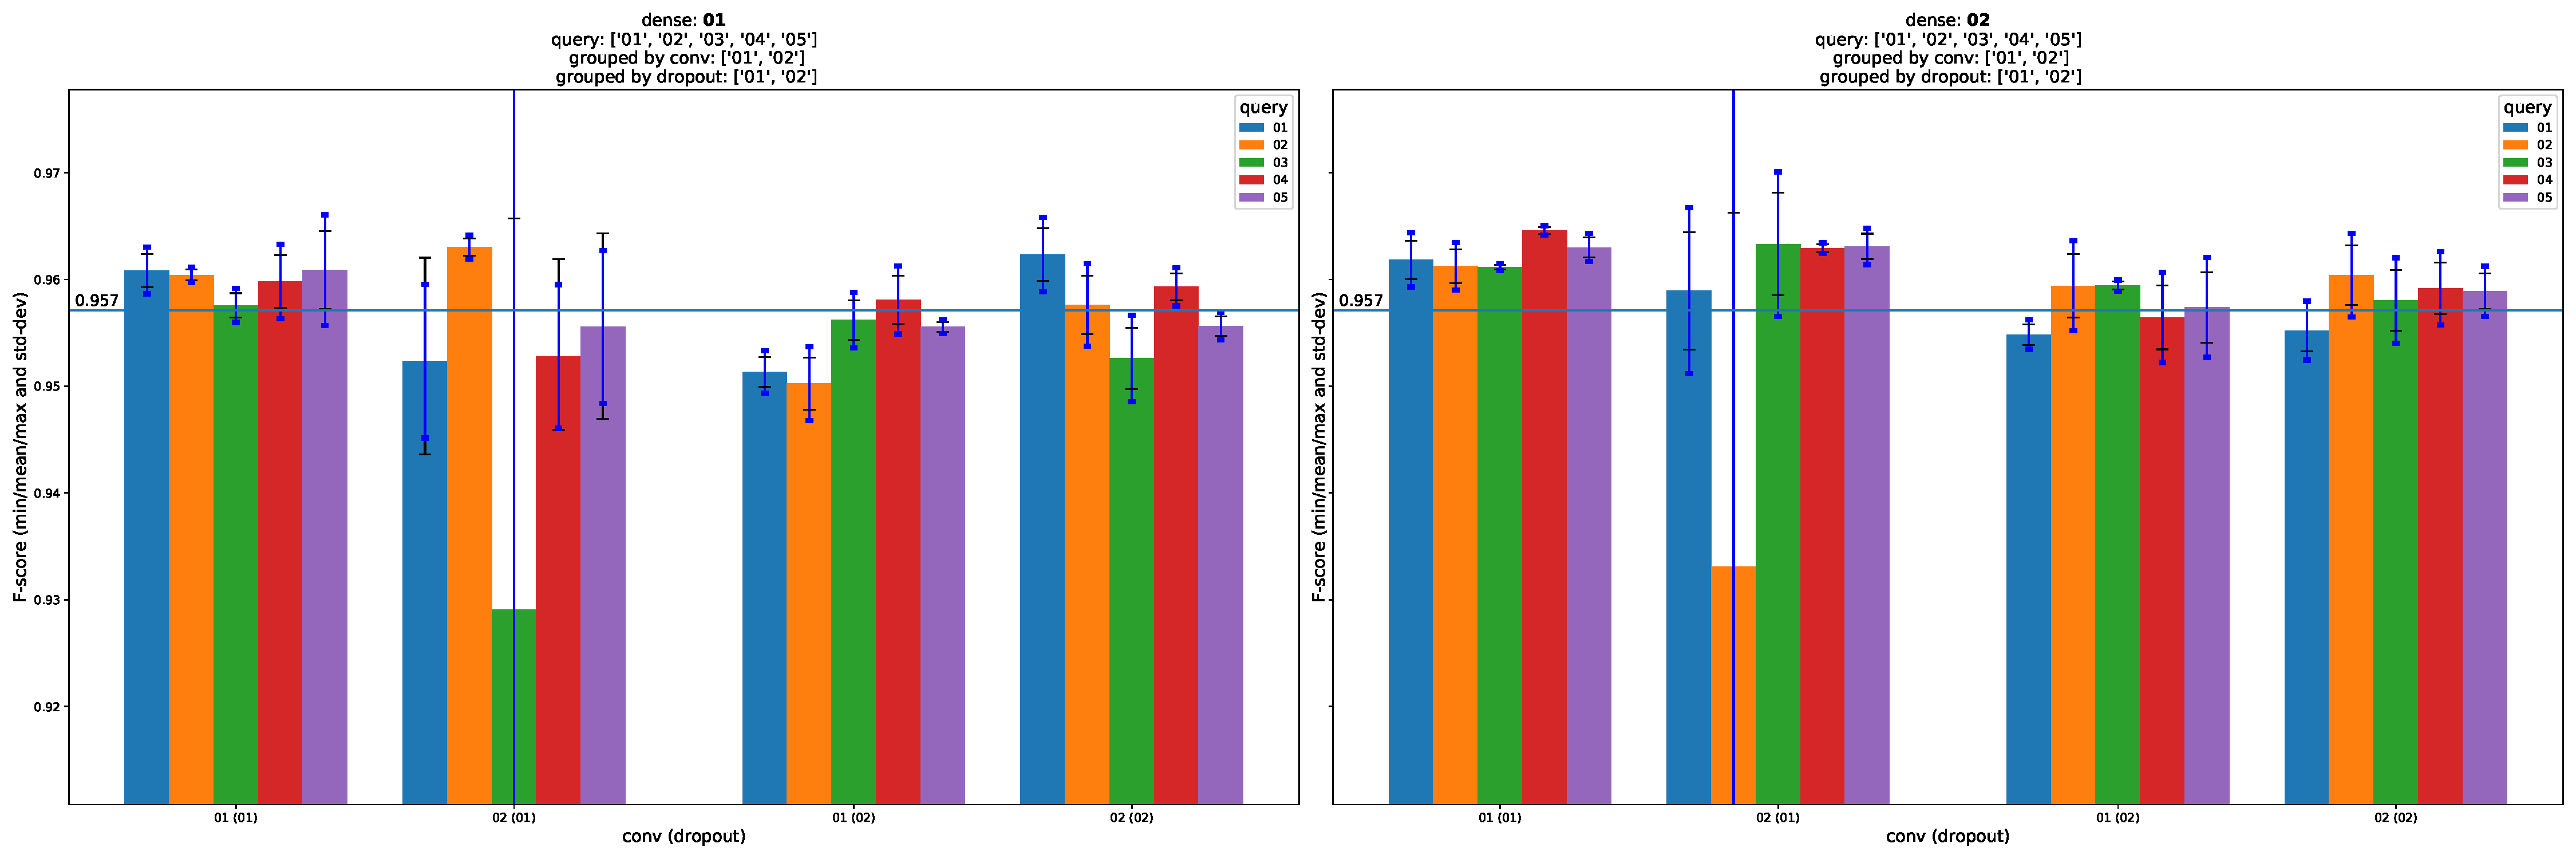
\includegraphics[width=0.9\linewidth]{Fscore_att2_dropout__conv__query__dense.pdf}
    \caption{F-score for varying
        dense classifier width,
        query type,
        convolution type,
        dropout.
        Averaged on 20 and 35 words task, solved by the LSTM+attention architecture.
        % MAYBE should also average on non ugmented dataset
        }%
    \label{fig:att_dropout_conv_query_dense}
\end{figure*}

\subsubsection{Training parameters performance comparison}

% Optimizer is fixed

\fig{fig:att_epoch_batch_lr_words} shows F-score values for 
variation of 
the number of training epochs ($2$, $4$, $15$ and $30$),
the batch size ($16$ or $32$),
and the learning rate
when the LSTM+attention model solves the task \texttt{k1}
on non-augmented datasets.
Two main conclusions can be reached:
\begin{itemize}
    \item
        The training gets more stable as the epoch number increases, and when
        using a larger batch size. For $30$ and $32$ respectively the results
        are quite consistent across the different learning rate types.
    \item
        The learning rate schedule \texttt{clr\_tri2\_04} (a cyclic learning
        rate with triangular 2 shape), when using enough epochs and a large
        batch size, is the one that performs the best.
\end{itemize}

\begin{figure*}[t!]
    \centering
    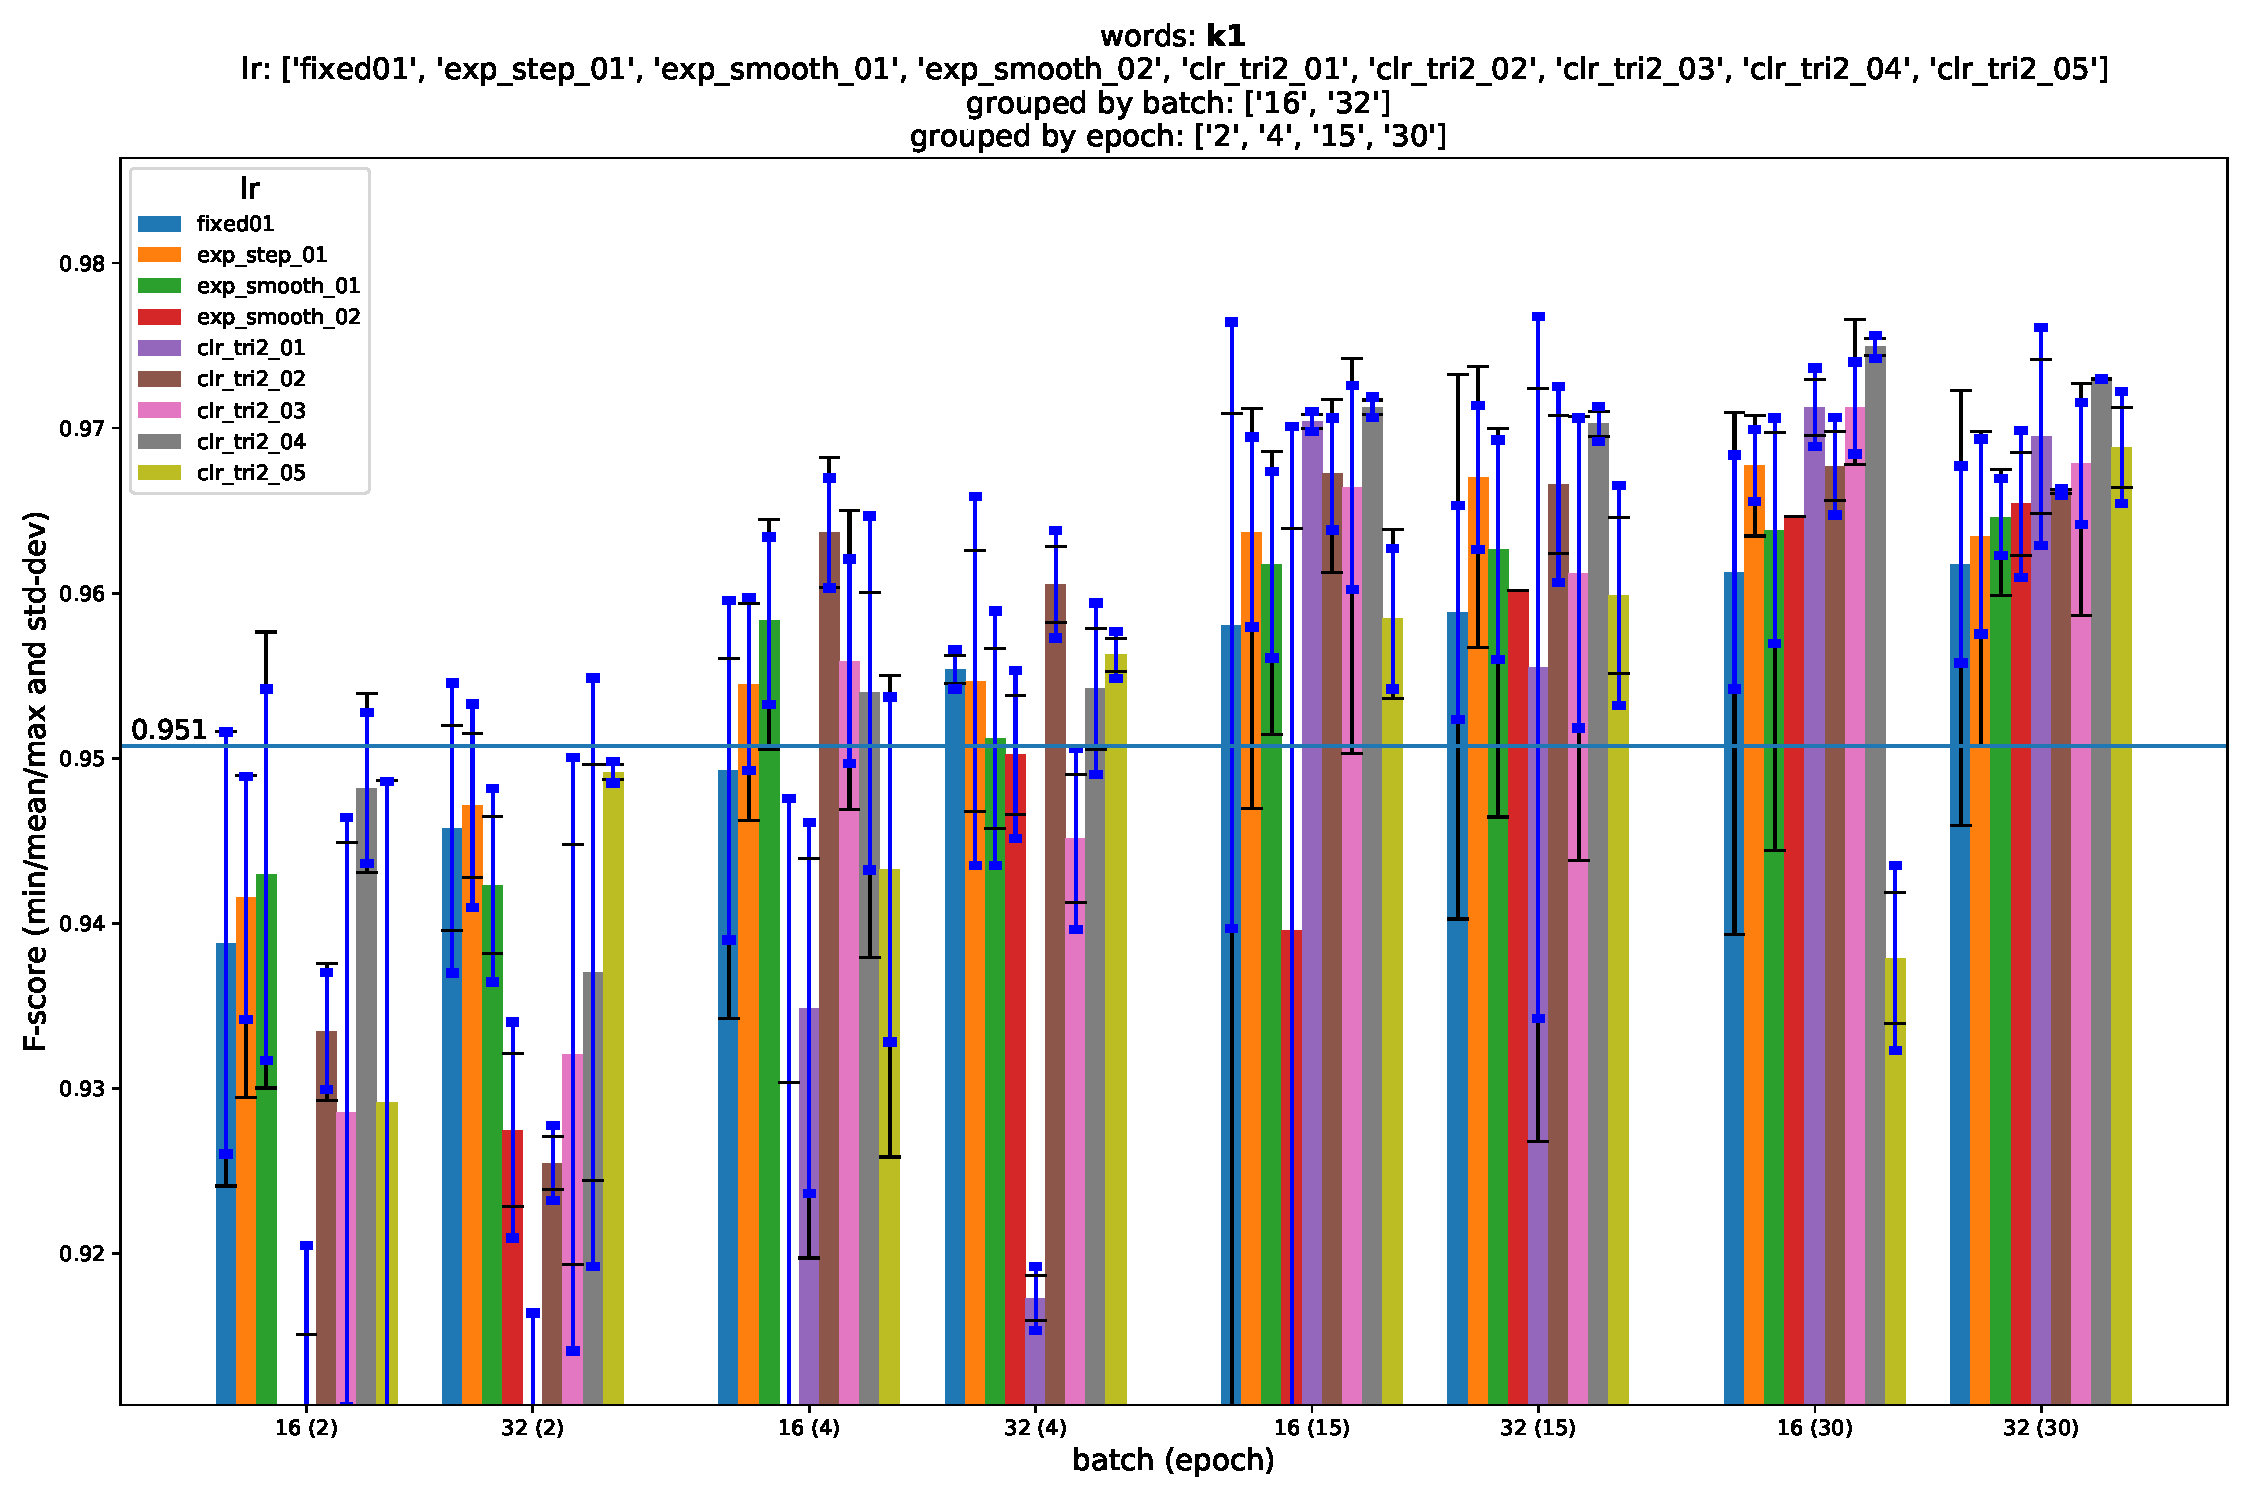
\includegraphics[width=0.9\linewidth]{Fscore_att2_epoch__batch__lr__words.pdf}
    \caption{F-score for varying
        epoch num,
        batch size,
        learning rate type,
        words type.
        Averaged on non-augmented datasets.
        Solved by the LSTM+attention architecture.
        }%
    \label{fig:att_epoch_batch_lr_words}
\end{figure*}

\subsection{AreaNet and SimpleNet performance}

TODO: So good!

\subsection{Data augmentation performance}
\label{sec:augmentation_performance}

% TODO: combine 01 and 15 for the final augmentation

As explained in \secref{sec:data_augmentation}, several types of augmentation
were performed on the dataset.
%
% MAYBE: type 01 aug was tested but too long The augmentation regarding the
% signal (i.e. \texttt{aug01}) was tested very little as it produced datasets
% that were too large to 
%
% The bulk of the investigation was to determine which kind of augmentation
% performed better.
Each type of augmentation is based on one set of spectrogram parameters, and
there are four styles of warp based aumentation: the landmarks are shifted 1)
along both axes of the spectrogram, 2) only along the time axis, 3) only along
the frequency axis, 4) along no axis, to provide a reference measure. Three
different spectrogram parameters and two different warping parameters were
tested. \tab{tab:aug_values}, in the Appendix, shows the specific values used.
For the ``big'' type, $3$ landmarks are shifted by at most $5$ units, while for
the ``small'' type, $4$ landmarks are shifted by at most $2$ units.
% The main differences in augmentation can be seen between the ``big'' and
% ``small'' types.
This leads to the largest difference in augmentation performance:
\tab{tab:augmentation_comparison_performance} shows that the ``small''
augmentation type leads to an increase in F-Score value of $0.015$ and $0.03$
relative to the ``big'' augmentation, when training the convolutional
architecture (\secref{sec:convolutional_arch}) on a 4-words task, and the
LSTM+attention model (\secref{sec:attention_model}) on a 10-words task
respectively.
%
This makes sense: the spectrograms used for augmentation have shape $(64, 64)$,
so moving a landmark by $5$ changes too sharply the image. A more uniform
augmentation, with more landmarks but with gentler warping leads to better
results.
%
For the convolutional architecture the mean F-Score value for the \texttt{f1}
4-words task increases from $0.939$ to $0.960$, while for the LSTM+attention
architecture, data augmentation does not increase the performance of the model.
However, the speed with which a high performance is achieved is influenced by
the presence of augmented data. As shown in
\tab{tab:augmentation_learning_speed} and in
\fig{fig:augmentation_learning_speed}, peak performance for the model is
reached after just $4$ epochs of training, compared to $10$ to $15$ epochs when
using non-augmented data.

\begin{table}[t!]
    \centering
    % \caption{Comparison between regular and augmented datasets:}
    \caption{Comparison between different types of augmentation,
    for the 10-words task solved by LSTM+attention architecture and a
    4-words task solved by the convolutional architecture.
    A reference non-augmented, well performing dataset is added.}
    \label{tab:augmentation_comparison_performance}
    \begin{tabular}{|cc|c|}
        \hline
        Aug ID & Spec+Type & F-Score \\
        \hline
        \hline
        % CNN & & (4 words)  \\
        % \multicolumn{2}{|c}{CNN} & (4 words) \\
        \multicolumn{3}{|c|}{CNN (4-words task)} \\
        % \hline
        % \hline
        % Aug ID & Spec+Type & F-Score \\
        \hline
        mel04 & None & $0.939 \pm 0.017$ \\
        02,03,04 & mel\_02+big   & $0.940 \pm 0.014$ \\
        06,07,08 & mel\_01+big   & $0.945 \pm 0.015$ \\
        10,11,12 & mel\_03+big   & $0.946 \pm 0.014$ \\
        14,15,16 & mel\_03+small & $0.960 \pm 0.008$ \\
        \hline
        \hline
        % \multicolumn{2}{c}{Multi-column}
        % LSTM+att & & (10 words) \\
        \multicolumn{3}{|c|}{LSTM+att (10-words task)} \\
        \hline
        % mel01   &  0.954 & 0.0073 \\
        mel04   &  None & $0.963 \pm 0.0126$ \\
        % mel05   & None &  $0.954 \pm 0.0184$ \\
        % mela1   &  0.958 & 0.0155 \\
        02,03,04 & mel\_02+big   &  $0.929 \pm 0.0362$ \\
        06,07,08 & mel\_01+big   &  $0.939 \pm 0.0392$ \\
        10,11,12 & mel\_03+big   &  $0.932 \pm 0.0852$ \\
        14,15,16 & mel\_03+small &  $0.964 \pm 0.0129$ \\
        \hline
    \end{tabular}
\end{table}

\begin{table}[t!]
    \centering
    \caption{Comparison of learning speed when training the LSTM+attention
    model on the $10$-words task \texttt{k1}.}
    \label{tab:augmentation_learning_speed}
    \begin{tabular}{|c|c|c|}
        \hline
        Epoch num & Regular & Augmented \\
        \hline
        2 & $0.923 \pm 0.034$ & $0.941 \pm 0.019$ \\
        4 & $0.948 \pm 0.016$ & $0.958 \pm 0.011$ \\
        15 & $0.959 \pm 0.013$ & $0.962 \pm 0.014$ \\
        \hline
    \end{tabular}
\end{table}

\begin{figure}[t!]
    \centering
    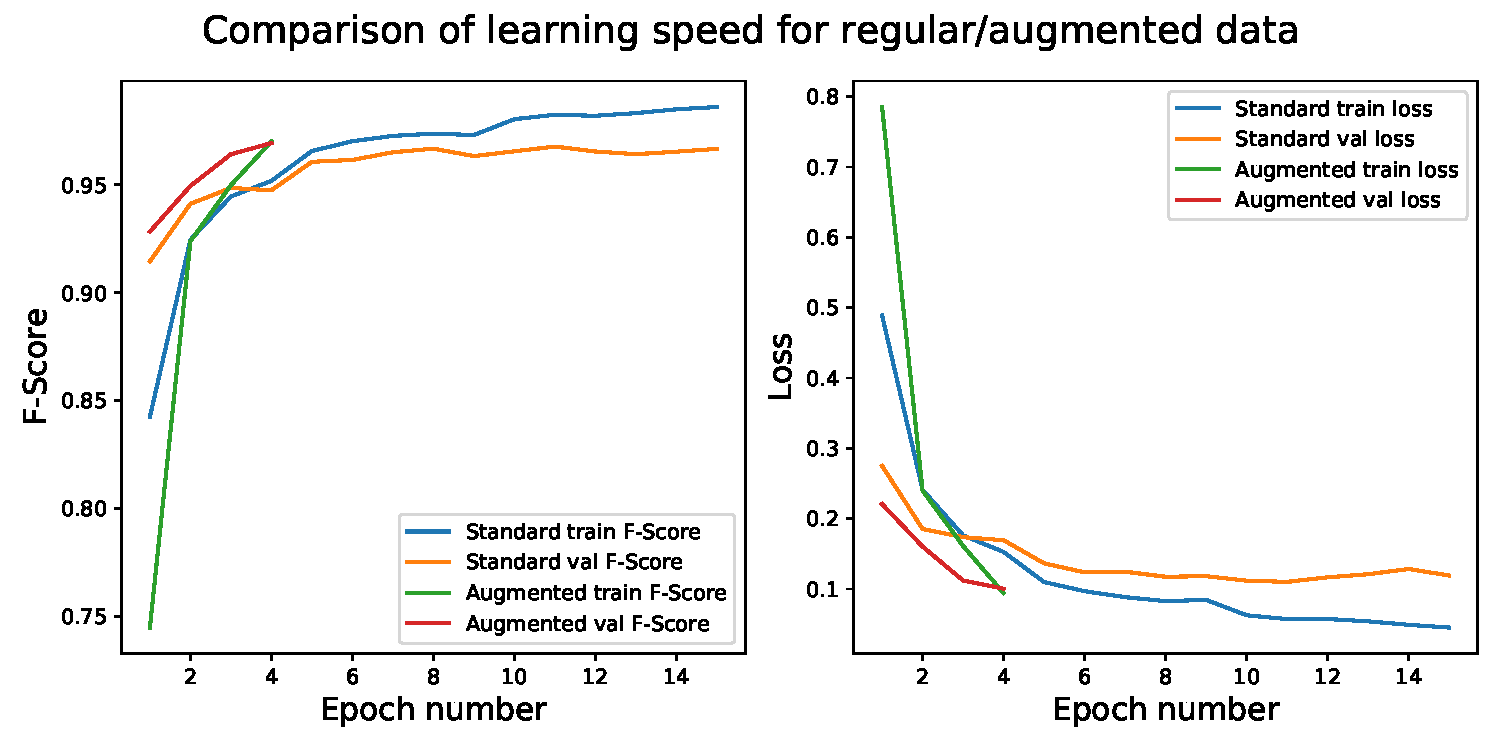
\includegraphics[width=0.9\linewidth]{comparison_augmentation.pdf}
    \caption{Comparison of the learning speed on regular vs. augmented data.}%
    \label{fig:augmentation_learning_speed}
\end{figure}

In \tab{tab:att_augmentation_comparison} the different types of
augmentation, along different axis, are compared:
no particular type emerges as better than the others.

\begin{table}[t!]
    \centering
    \caption{Comparison between different styles of augmentation,
    for the 10-words task solved by LSTM+attention architecture and a
    4-words task solved by the convolutional architecture.}
    \label{tab:att_augmentation_comparison}
    \begin{tabular}{|c|c|}
        \hline
        Augmentation type & F-Score \\
        \hline
        \hline
        \multicolumn{2}{|c|}{LSTM+attention (10 words task)} \\
        \hline
        Both axis & $0.9326 \pm 0.0615$ \\
        Time      & $0.9448 \pm 0.0323$ \\
        Frequency & $0.9355 \pm 0.0383$ \\
        None      & $0.9311 \pm 0.0794$ \\
        \hline
        \hline
        \multicolumn{2}{|c|}{CNN (4 words task)} \\
        \hline
        Both axis & $0.945 \pm 0.016$ \\
        Time      & $0.946 \pm 0.014$ \\
        Frequency & $0.944 \pm 0.014$ \\
        None      & $0.940 \pm 0.016$ \\
        \hline
    \end{tabular}
\end{table}

%%%%%%%%%%%%%%%%%%%

\subsection{Extract loudest section performance}

As an additional preprocessing step, the loudest $0.5$s section of the audio
signal was selected.
%
It might seem surprising, but both the LSTM+attention and the AreaNet
architectures performed better on the full audio samples, 
as shown in \tab{tab:comparison_loud_section}.
%
This however could partly be explained by the fact that those are \textit{attention}
architectures, so by design they will identify the relevant portion of the data.
By only feeding important data to the networks, the attention mechanism has more
difficulty to learn which sections to select, because all of them are useful.
%
On the other hand, the SimpleNet was also trained on the loudest section of the data
and that also did not lead to an improvement.
% MAYBE

\begin{table}[t!]
    \centering
    \caption{Comparison of the original dataset and the dataset that only
    includes the loudest section of the audio samples.}
    \label{tab:comparison_loud_section}
    \begin{tabular}{|c|c|c|}
        \hline
        & LTnum & LTnumLS \\
        \hline
        CNN      & $0.967 \pm 0.000$ & $0.952 \pm 0.003$ \\
        LSTM+att & $0.969 \pm 0.012$ & $0.953 \pm 0.012$ \\
        AreaNet  & $0.977 \pm 0.011$ & $0.962 \pm 0.023$ \\
        \hline
        % & LSTM+att & AreaNet(s) \\
        % LTnum   & $0.969 \pm 0.012$ & $0.977 \pm 0.011$ \\
        % LTnumLS & $0.953 \pm 0.012$ & $0.962 \pm 0.023$ \\
    \end{tabular}
\end{table}

\subsection{Architecture comparison}

TODO:

Show best and top 5 average

Then aggregate table for cross architecture

Pick the best 5 models per category for each task

Compare: CNN, Dense, Xception, EfficientB047, LSTM+attention, AreaNet, SimpleNet,
VerticalAreaNet on num, all, LTnum, LTall, numLS, allLS

Not every combination of everything

Show confusion matrices, speak about similar sounding words, note how AreaNet
does not miss them

% % Autogenerated by python evaluate_all.py -et build_megacomparison_v03
% Mildly modified
\begin{table*}[t!]
    \centering
    \caption{Architecture comparison for different tasks. Each cell shows the mean, standard deviation and max F-Score value.}
    \label{tab:mega_comparison}
    \begin{tabular}{|c|ccccc|}
        \hline
        Arch & f1 & k1 & yn & num, LTnum, LTBnum & all, LTall, LTBall \\
        \hline
        \hline
        \multirow{2}{*}{CNN}
             & $0.918 \pm 0.037$ & -                 & -                 & $0.955 \pm 0.010$ & $0.879 \pm 0.040$ \\
             & $    0.980 $      & -                 & -                 & $    0.970 $      & $    0.909 $      \\
        \hline
        \multirow{2}{*}{TRA}
             & $0.878 \pm 0.091$ & -                 & $0.977 \pm 0.002$ & $0.945 \pm 0.009$ & -                 \\
             & $    0.953 $      & -                 & $    0.978 $      & $    0.951 $      & -                 \\
        \cline{2-6}
        \multirow{2}{*}{TD1}
             & $0.960 \pm 0.024$ & $0.959 \pm 0.008$ & $0.988 \pm 0.003$ & $0.970 \pm 0.008$ & $0.948 \pm 0.003$ \\
             & $    0.980 $      & $    0.964 $      & $    0.990 $      & $    0.977 $      & $    0.950 $      \\
        \cline{2-6}
        \multirow{2}{*}{TB0}
             & $0.844 \pm 0.105$ & $0.898 \pm 0.035$ & -                 & $0.938 \pm 0.016$ & $0.902 \pm 0.001$ \\
             & $    0.907 $      & $    0.919 $      & -                 & $    0.946 $      & $    0.903 $      \\
        \cline{2-6}
        \multirow{2}{*}{TB4}
             & $0.955 \pm 0.003$ & -                 & $0.994 \pm 0.000$ & $0.954 \pm 0.003$ & $0.910 \pm 0.002$ \\
             & $    0.957 $      & -                 & $    0.994 $      & $    0.958 $      & $    0.911 $      \\
        \cline{2-6}
        \multirow{2}{*}{TB7}
             & $0.966 \pm 0.000$ & -                 & -                 & -                 & -                 \\
             & $    0.966 $      & -                 & -                 & -                 & -                 \\
        \hline
        \multirow{2}{*}{ATT}
             & $0.962 \pm 0.011$ & $0.946 \pm 0.033$ & $0.988 \pm 0.010$ & $0.969 \pm 0.012$ & $0.948 \pm 0.003$ \\
             & $    0.978 $      & $    0.977 $      & $    0.996 $      & $    0.978 $      & $    0.952 $      \\
        \hline
        \multirow{2}{*}{SIM}
             & $0.982 \pm 0.005$ & $0.975 \pm 0.002$ & $0.995 \pm 0.004$ & $0.981 \pm 0.003$ & $0.953 \pm 0.006$ \\
             & $    0.989 $      & $    0.978 $      & $\bf{0.999}$      & $    0.986 $      & $    0.960 $      \\
        \cline{2-6}
        \multirow{2}{*}{SI2}
             & $0.984 \pm 0.004$ & $0.978 \pm 0.003$ & $0.997 \pm 0.002$ & $0.984 \pm 0.003$ & $0.963 \pm 0.002$ \\
             & $\bf{0.990}$      & $\bf{0.982}$      & $\bf{0.999}$      & $\bf{0.988}$      & $\bf{0.967}$      \\
        \cline{2-6}
        \multirow{2}{*}{AAN}
             & $0.947 \pm 0.028$ & $0.879 \pm 0.102$ & $0.940 \pm 0.113$ & $0.971 \pm 0.020$ & $0.948 \pm 0.010$ \\
             & $    0.979 $      & $    0.954 $      & $    0.996 $      & $    0.985 $      & $    0.962 $      \\
        \cline{2-6}
        \multirow{2}{*}{VAN}
             & $0.964 \pm 0.018$ & $0.969 \pm 0.005$ & $0.950 \pm 0.094$ & $0.975 \pm 0.011$ & $0.948 \pm 0.013$ \\
             & $    0.979 $      & $    0.978 $      & $\bf{0.999}$      & $    0.986 $      & $    0.961 $      \\
        \hline
    \end{tabular}
\end{table*}


% Autogenerated by python evaluate_all.py -et evaluate_results_all
\begin{table*}[t!]
    \centering
    \caption{Mega comparison}
    \label{tab:mega_comparison}
    \begin{tabular}{|c|ccc|}
        \hline
        \multicolumn{4}{|c|}{Task: f1} \\
        \hline
        Arch & Mean $\pm$ StdDev & Min & Max \\
        \hline
        CNN & $0.832 \pm 0.109$ & $0.501$ & $0.978$ \\
        TRA & $0.868 \pm 0.099$ & $0.521$ & $0.953$ \\
        TD1 & $0.960 \pm 0.024$ & $0.920$ & $0.980$ \\
        TB0 & $0.844 \pm 0.105$ & $0.687$ & $0.907$ \\
        TB4 & $0.955 \pm 0.003$ & $0.951$ & $0.957$ \\
        TB7 & $0.966 \pm 0.000$ & $0.966$ & $0.966$ \\
        ARN & $0.979 \pm 0.011$ & $0.960$ & $\bf{0.986}$ \\
        \hline
        \hline
        \multicolumn{4}{|c|}{Task: k1} \\
        \hline
        Arch & Mean $\pm$ StdDev & Min & Max \\
        \hline
        TD1 & $0.959 \pm 0.008$ & $0.950$ & $0.964$ \\
        TB0 & $0.898 \pm 0.035$ & $0.847$ & $0.919$ \\
        ATT & $0.946 \pm 0.031$ & $0.729$ & $\bf{0.977}$ \\
        \hline
        \hline
        \multicolumn{4}{|c|}{Tasks: yn, LTyn} \\
        \hline
        Arch & Mean $\pm$ StdDev & Min & Max \\
        \hline
        AAN & $0.941 \pm 0.131$ & $0.529$ & $0.990$ \\
        ARN & $0.997 \pm 0.003$ & $0.995$ & $\bf{0.999}$ \\
        SIM & $0.992 \pm 0.003$ & $0.987$ & $0.998$ \\
        VAN & $0.991 \pm 0.004$ & $0.986$ & $0.998$ \\
        \hline
        \hline
        \multicolumn{4}{|c|}{Tasks: num, LTnum} \\
        \hline
        Arch & Mean $\pm$ StdDev & Min & Max \\
        \hline
        CNN & $0.954 \pm 0.012$ & $0.828$ & $0.970$ \\
        TRA & $0.945 \pm 0.009$ & $0.939$ & $0.951$ \\
        TD1 & $0.970 \pm 0.008$ & $0.960$ & $0.977$ \\
        TB0 & $0.938 \pm 0.016$ & $0.914$ & $0.946$ \\
        TB4 & $0.954 \pm 0.003$ & $0.951$ & $0.958$ \\
        ATT & $0.969 \pm 0.012$ & $0.911$ & $0.978$ \\
        AAN & $0.962 \pm 0.025$ & $0.917$ & $0.985$ \\
        ARN & $0.981 \pm 0.002$ & $0.978$ & $0.983$ \\
        SIM & $0.981 \pm 0.003$ & $0.975$ & $0.985$ \\
        SI2 & $0.981 \pm 0.004$ & $0.975$ & $\bf{0.986}$ \\
        VAN & $0.975 \pm 0.006$ & $0.964$ & $0.981$ \\
        \hline
        \hline
        \multicolumn{4}{|c|}{Tasks: all, LTall} \\
        \hline
        Arch & Mean $\pm$ StdDev & Min & Max \\
        \hline
        CNN & $0.863 \pm 0.057$ & $0.653$ & $0.901$ \\
        TD1 & $0.948 \pm 0.003$ & $0.946$ & $0.950$ \\
        TB0 & $0.902 \pm 0.001$ & $0.901$ & $0.903$ \\
        TB4 & $0.910 \pm 0.002$ & $0.908$ & $0.911$ \\
        ATT & $0.949 \pm 0.003$ & $0.946$ & $0.952$ \\
        AAN & $0.948 \pm 0.010$ & $0.927$ & $0.957$ \\
        ARN & $0.952 \pm 0.005$ & $0.944$ & $0.957$ \\
        SIM & $0.954 \pm 0.004$ & $0.948$ & $0.960$ \\
        SI2 & $0.963 \pm 0.001$ & $0.960$ & $\bf{0.965}$ \\
        VAN & $0.953 \pm 0.009$ & $0.932$ & $0.961$ \\
        \hline
    \end{tabular}
\end{table*}

\subsection{FSDD performance}

TODO: Test all on that, MAYBE merge with architecture comparision

\subsection{Attention weights}

% \subsubsection{Attention model}

% Show attention weights for Att model

The LSTM+attention model described in \secref{sec:attention_model} computes a query
vector that is used to weigh the LSTM outputs. Showing the attention weights
can help understand which parts of the recording were relevant for the
classification.
\fig{fig:attention_weights_standard} shows the spectrograms, the attention
weigths and the predictions for three sample words.
Indeed, the attention weights show which some sections of the data is more important
and is used to extract information from the signal.

% ATT_ct02_dr01_ks01_lu01_qt05_dw01_opa1_lr03_bs02_en02_dsaug07_wLTnum_LTnum_train_data
\begin{figure*}[t!]
    \centering
    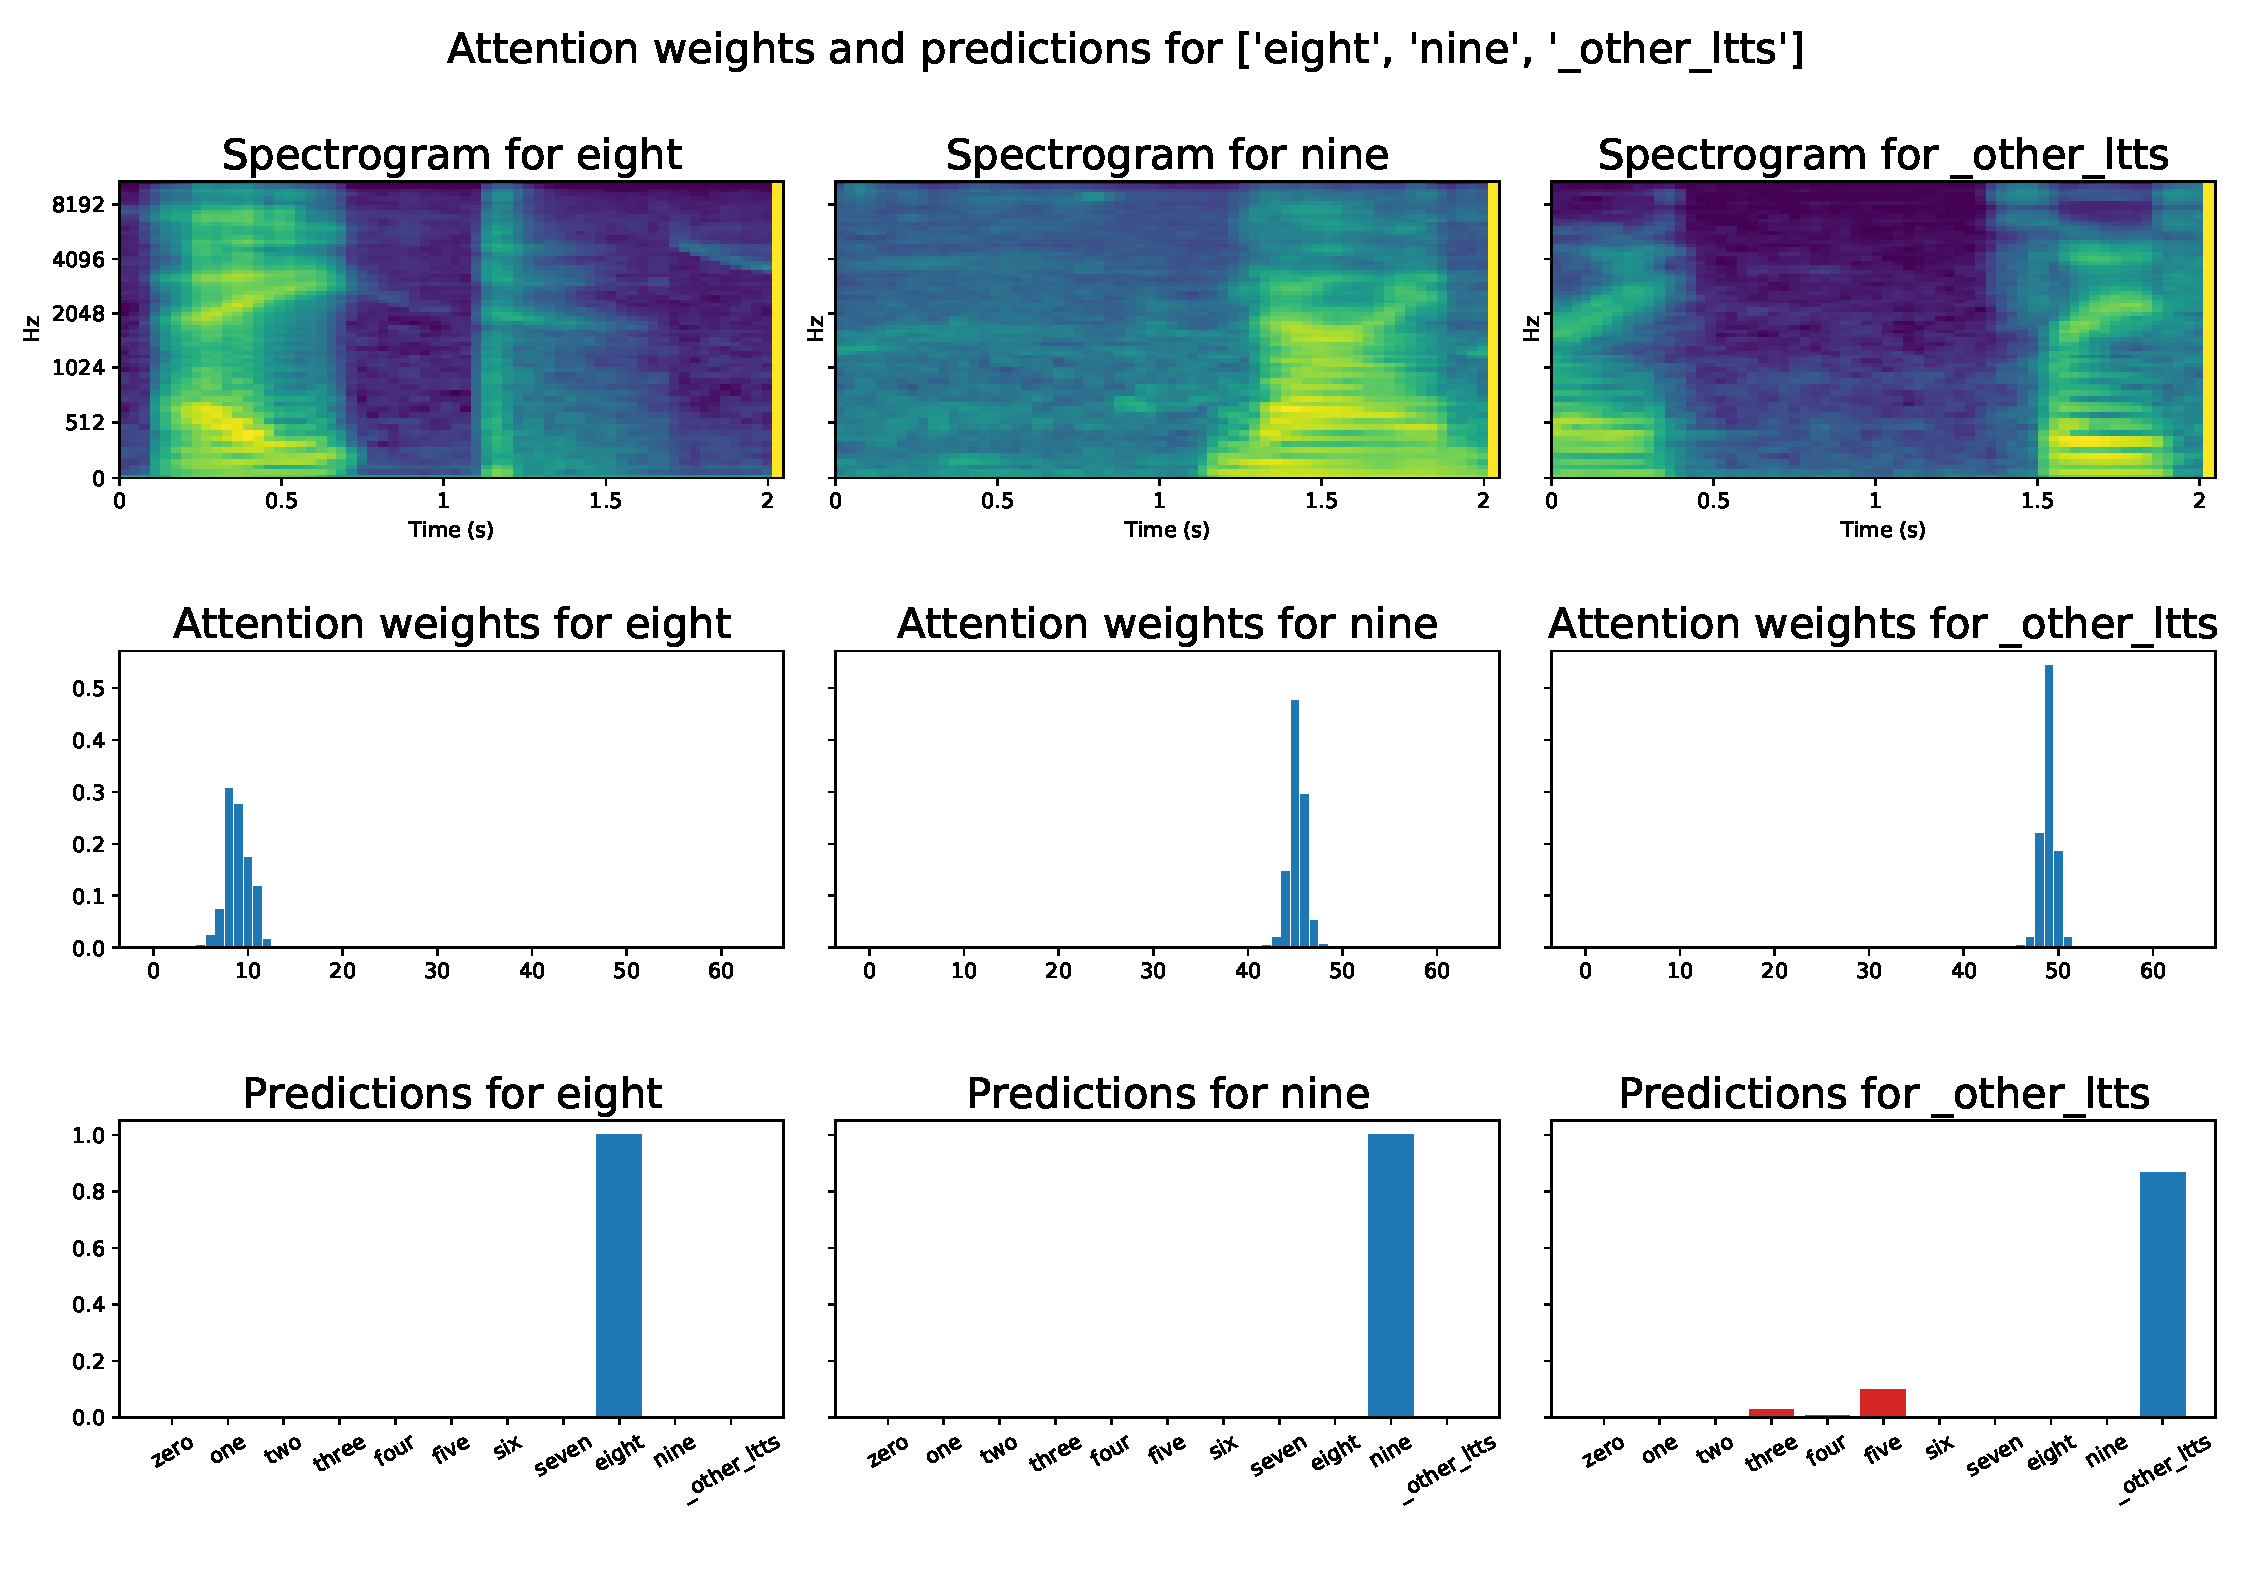
\includegraphics[width=0.9\linewidth]{ATT_ct02_dr01_ks01_lu01_qt05_dw01_opa1_lr03_bs02_en02_dsaug07_wLTnum_LTnum_train_data.pdf}
    \caption{Spectrograms, attention weights and predictions for three sample words.
    Notice how the attention weights correctly selected the interesting part of
    the ``eight'' spectrogram, avoiding the noise in the latter part.
    For ``\_other\_ltts'', which corresponds to a random audio snippet from the LibriTTS
    dataset, the attention weights still selected the section where a word is spoken,
    and, with some small uncertainty, the word is indeed recognized as ``other''.}%
    \label{fig:attention_weights_standard}
\end{figure*}

An example of the weights computed by AreaNet and VerticalAreaNet were already shown 
in \fig{fig:attention_weights_area} and \fig{fig:attention_weights_vertical}.

\subsection{Stream predictions}

The effectiveness of using a model trained on single word utterances to
identify a word in a sentence is examined in this section.
\fig{fig:stream_attention_ltts_meL04_LTnumLS_26} is an example of a very good
scenario: of the four numbers spoken, three are well isolated in the sentence,
and are clearly picked up. The initial utterance of ``three'' is also
identified, albeit with a lower probability, as it is very close to the next
word (``\textit{three} o'clock'' is spoken with barely a pause).
\fig{fig:stream_attention_ltts_meL04_LTnumLS_67} shows a more common situation,
when the interesting word is in the middle of the sentence (``of the
\textit{four} other\ldots''). The model can only barely identify the presence
of the word.
\fig{fig:stream_attention_ltts_meL04_LTnumLS_19} shows why a ``silence'' class
would be useful: when background converation is present, the model consistently
identifies \texttt{\_other} as the predicted word, but in the section where no
word is spoken, the model fires randomly.

Training only on the loudest $0.5$ second section of the audio samples improves
the performance of the models quite a lot: the ``four'' in the second example
is completely missed by a model trained with identical parameters except the
longer words, as shown in \fig{fig:stream_attention_ltts_mel04_LTnum_67}: only
the more isolated ``two'' is found, as there is space to align a window that
ends with the utterance and starts with silence.

A manual inspection was conducted on $116$ sentences containing numbers, and
only $31$ were correctly identified, amounting to $26.7\%$ recall.
The false positives however are only $14$, resulting in a precision of
$87.9\%$: if a number is identified, there is reasonable confidence that was
actually spoken.
% good_count: 31
% bad_count: 85
% total: 116

\begin{figure}[h!]
    \centering
    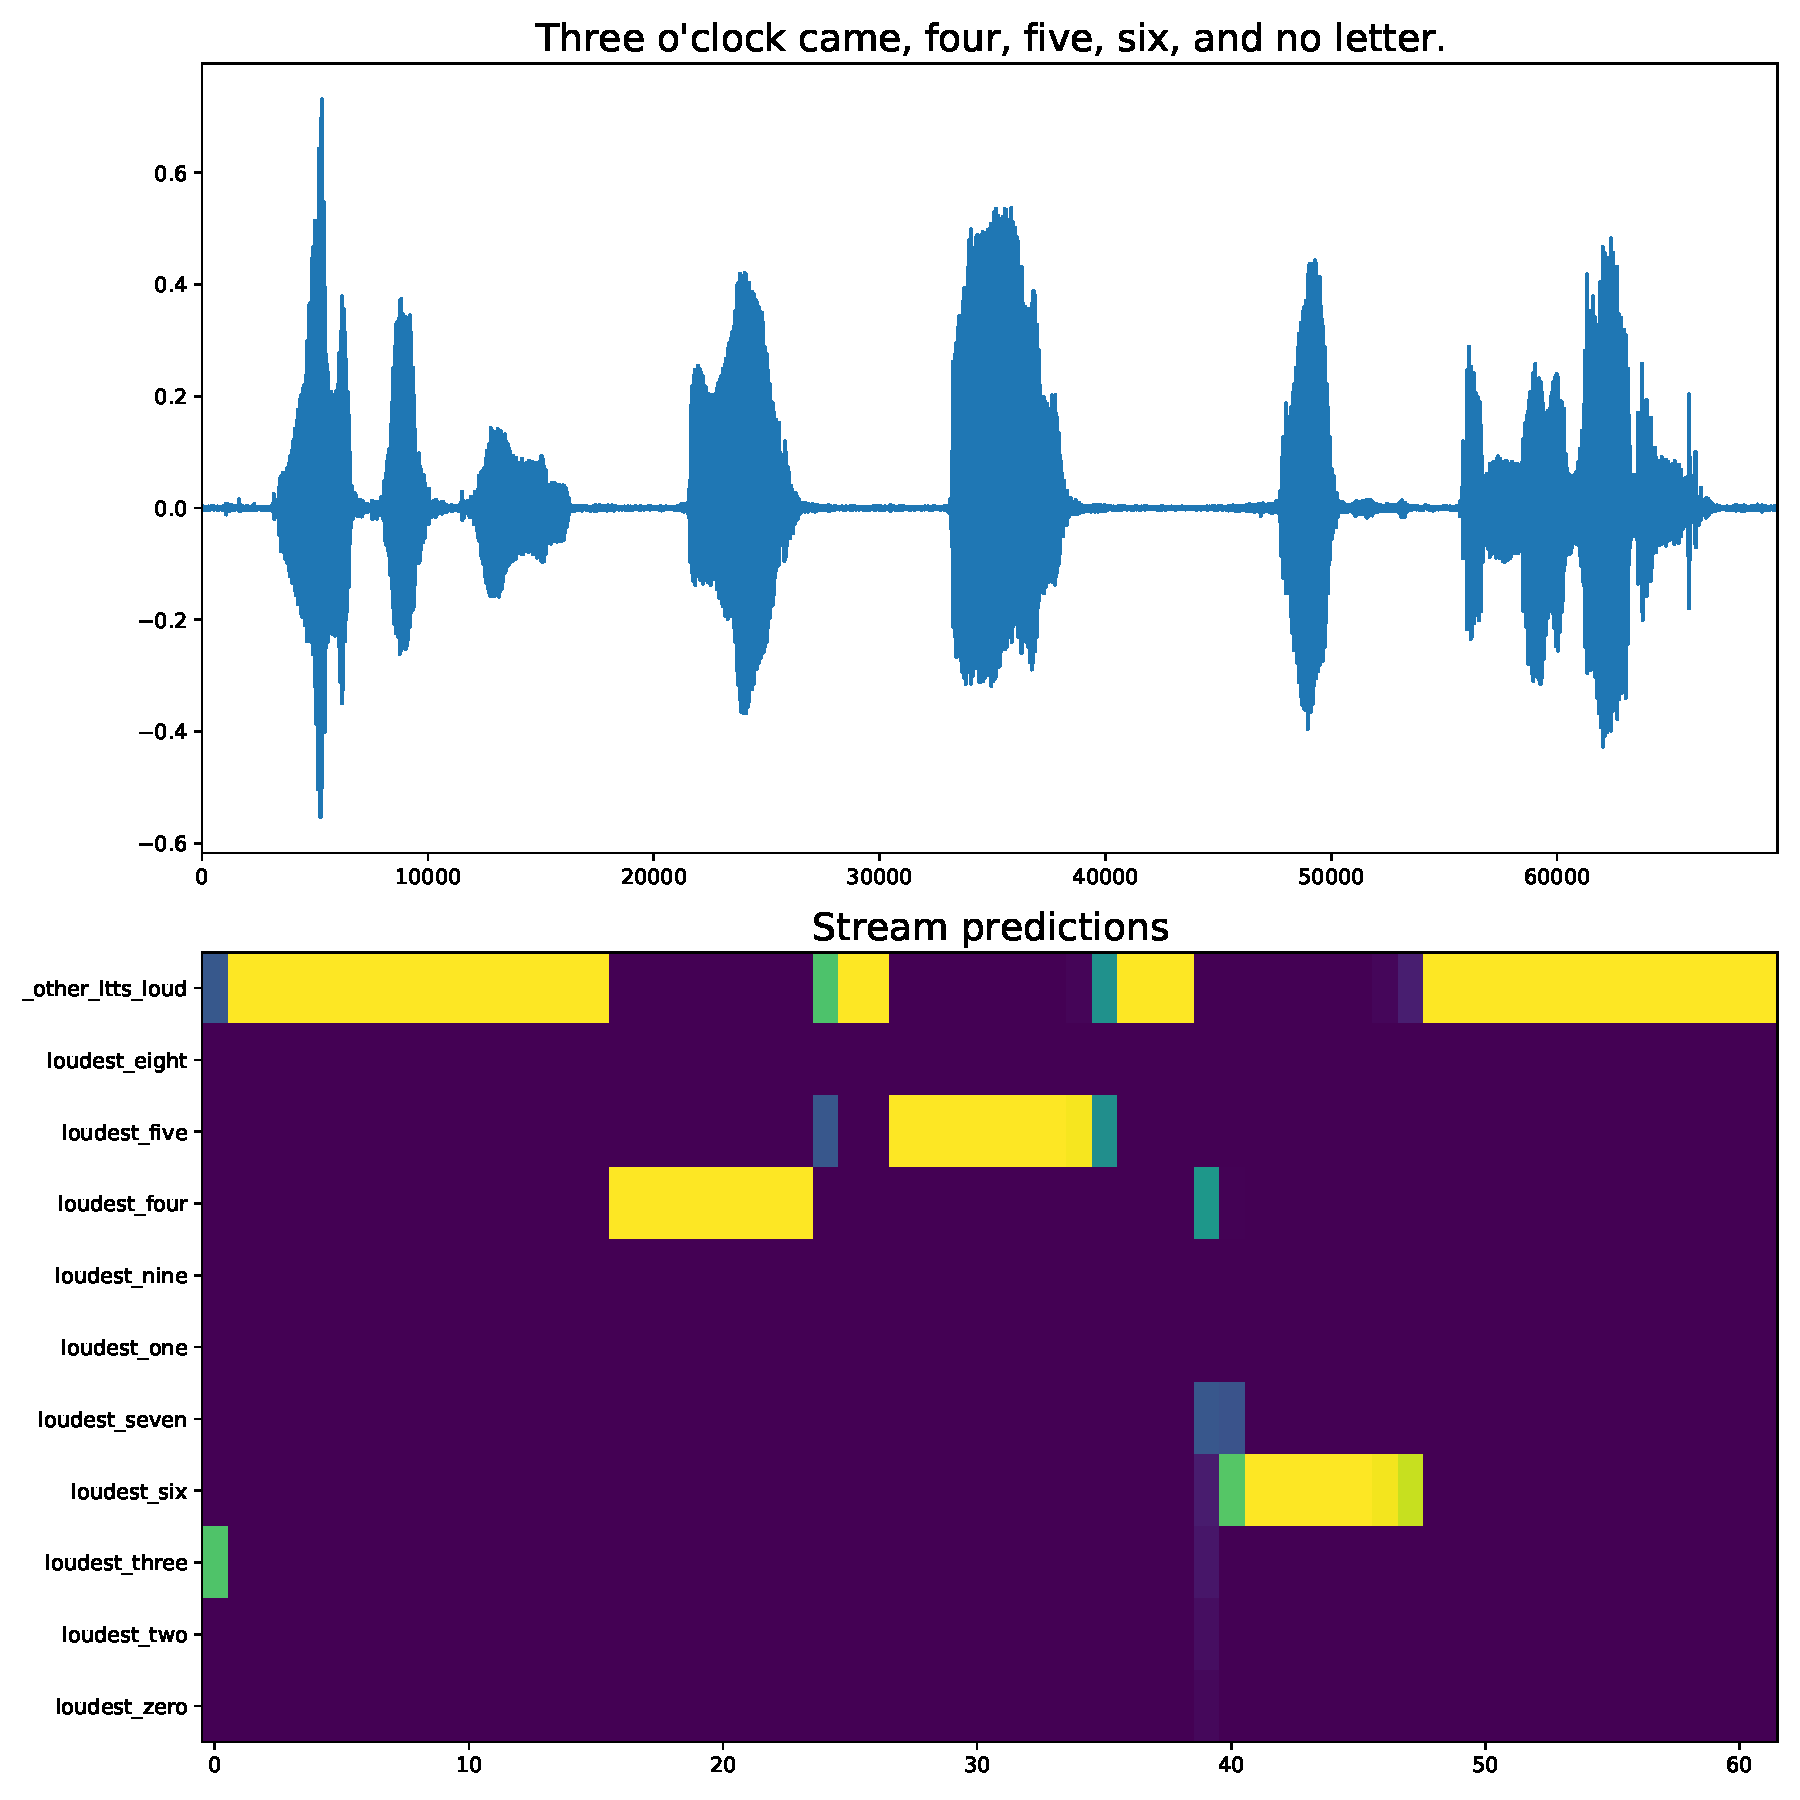
\includegraphics[width=0.9\linewidth]{stream2_attention_ltts_meL04_LTnumLS_26.pdf}
    \caption{Stream 26}%
    \label{fig:stream_attention_ltts_meL04_LTnumLS_26}
\end{figure}

\begin{figure}[h!]
    \centering
    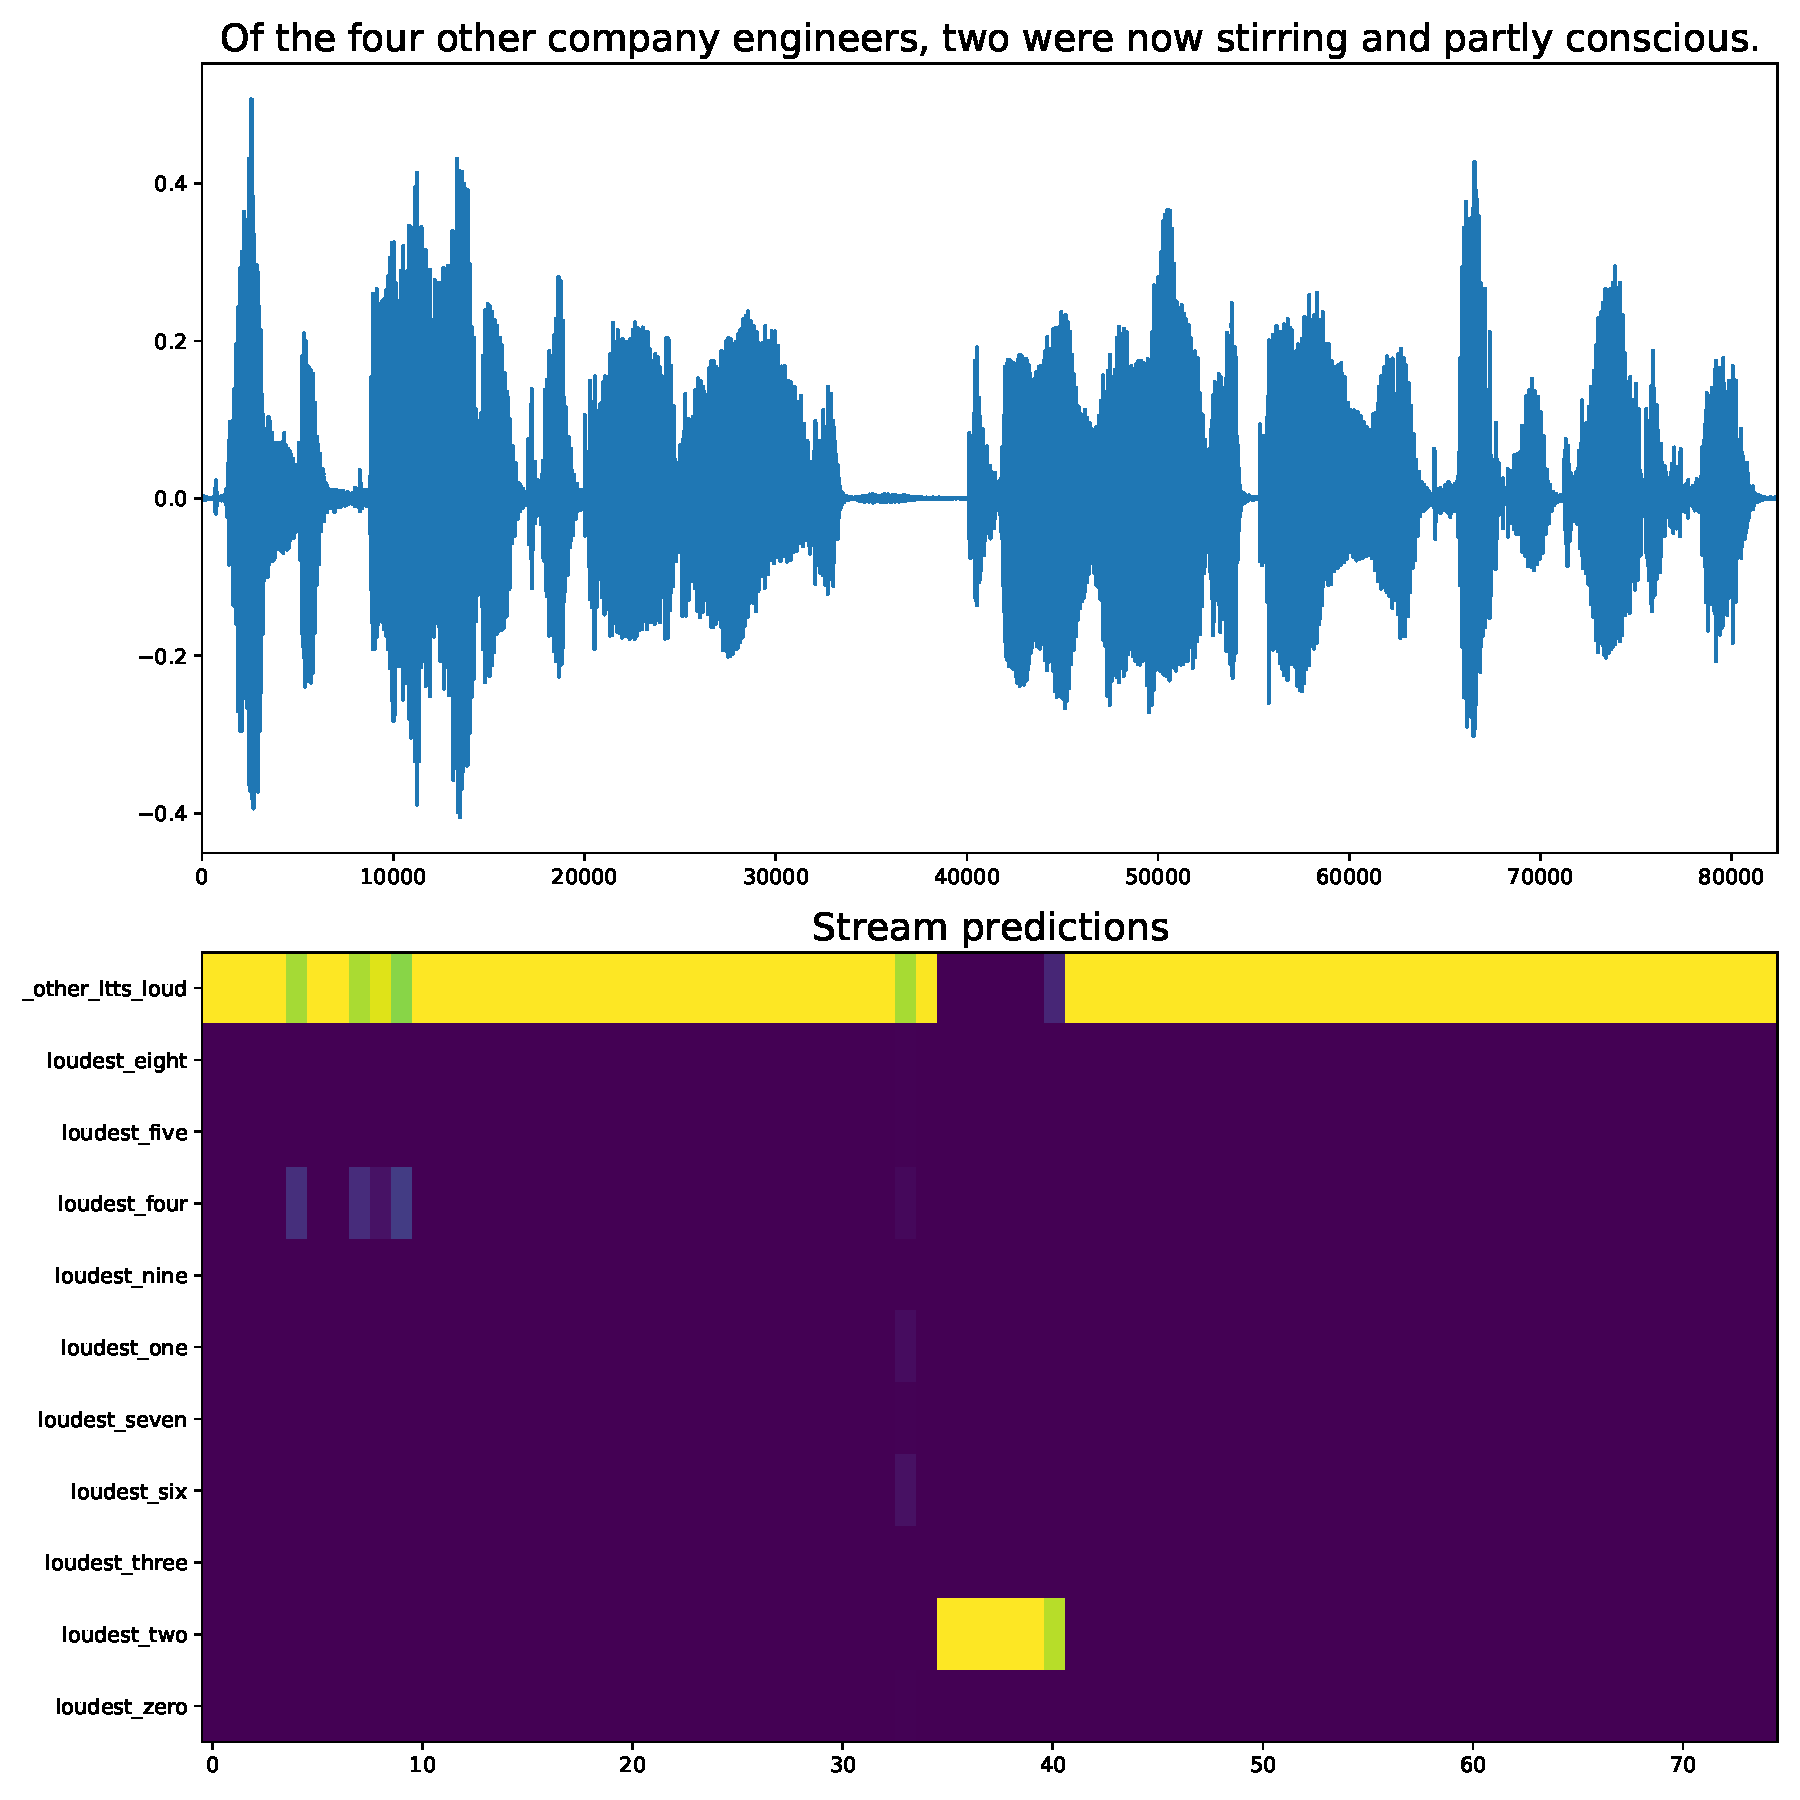
\includegraphics[width=0.9\linewidth]{stream2_attention_ltts_meL04_LTnumLS_67.pdf}
    \caption{Stream 67}%
    \label{fig:stream_attention_ltts_meL04_LTnumLS_67}
\end{figure}

\begin{figure}[h!]
    \centering
    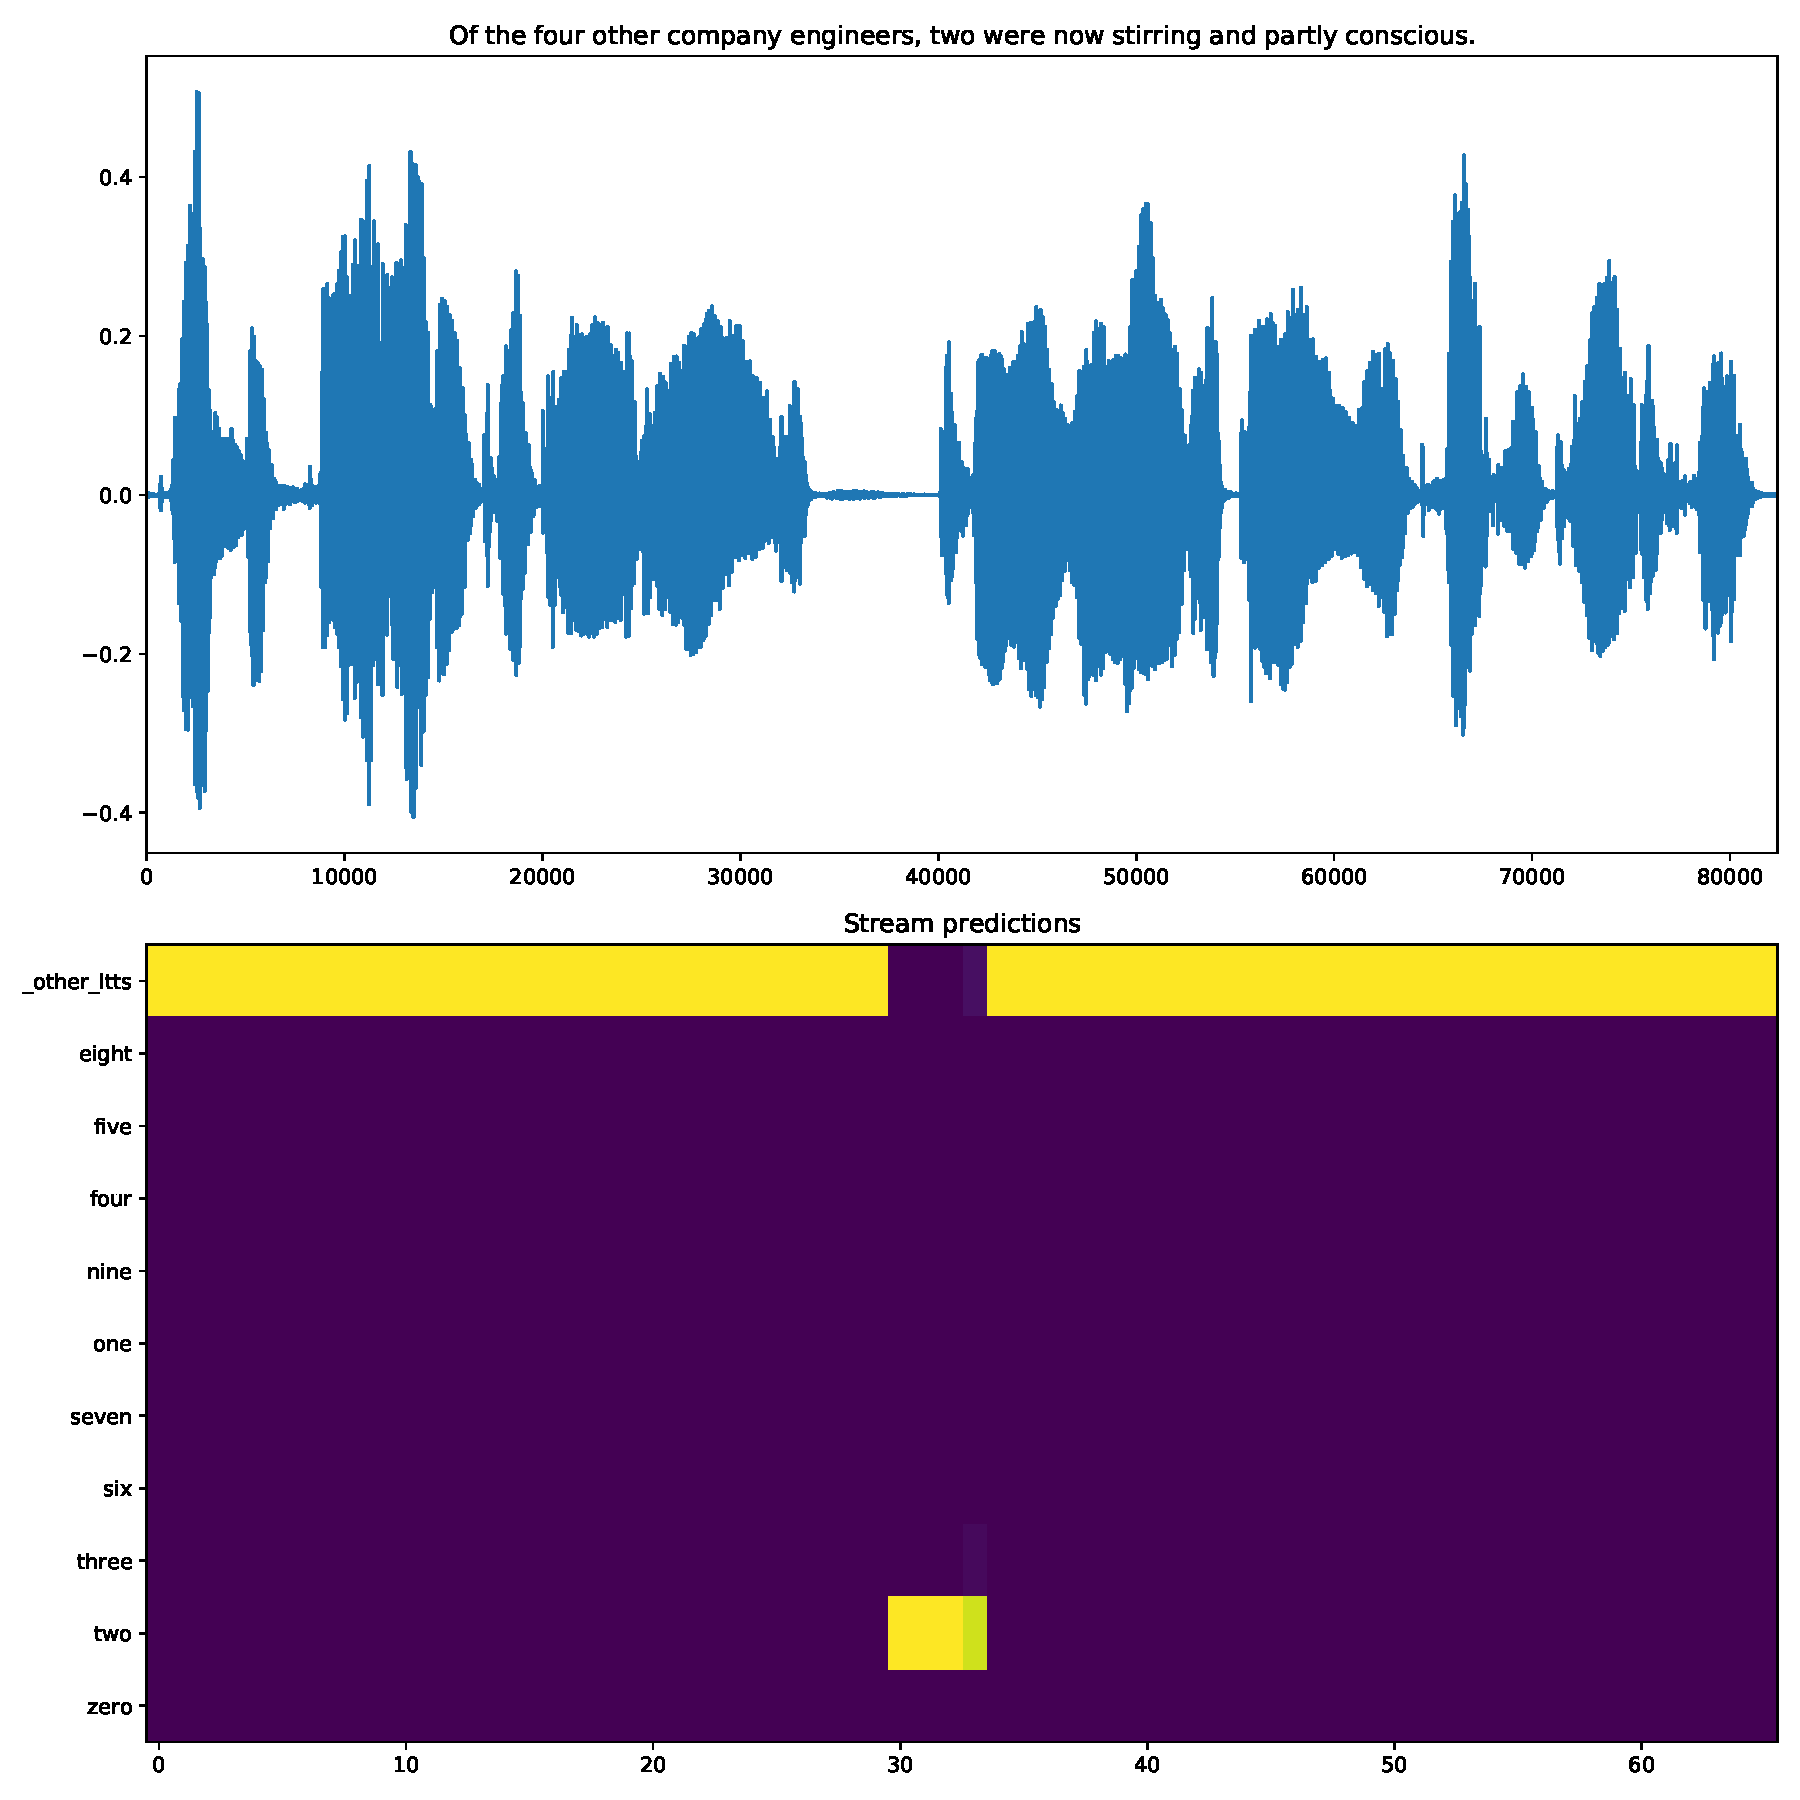
\includegraphics[width=0.9\linewidth]{stream_attention_ltts_mel04_LTnum_67.pdf}
    \caption{Stream 67 long words}%
    \label{fig:stream_attention_ltts_mel04_LTnum_67}
\end{figure}

\begin{figure}[h!]
    \centering
    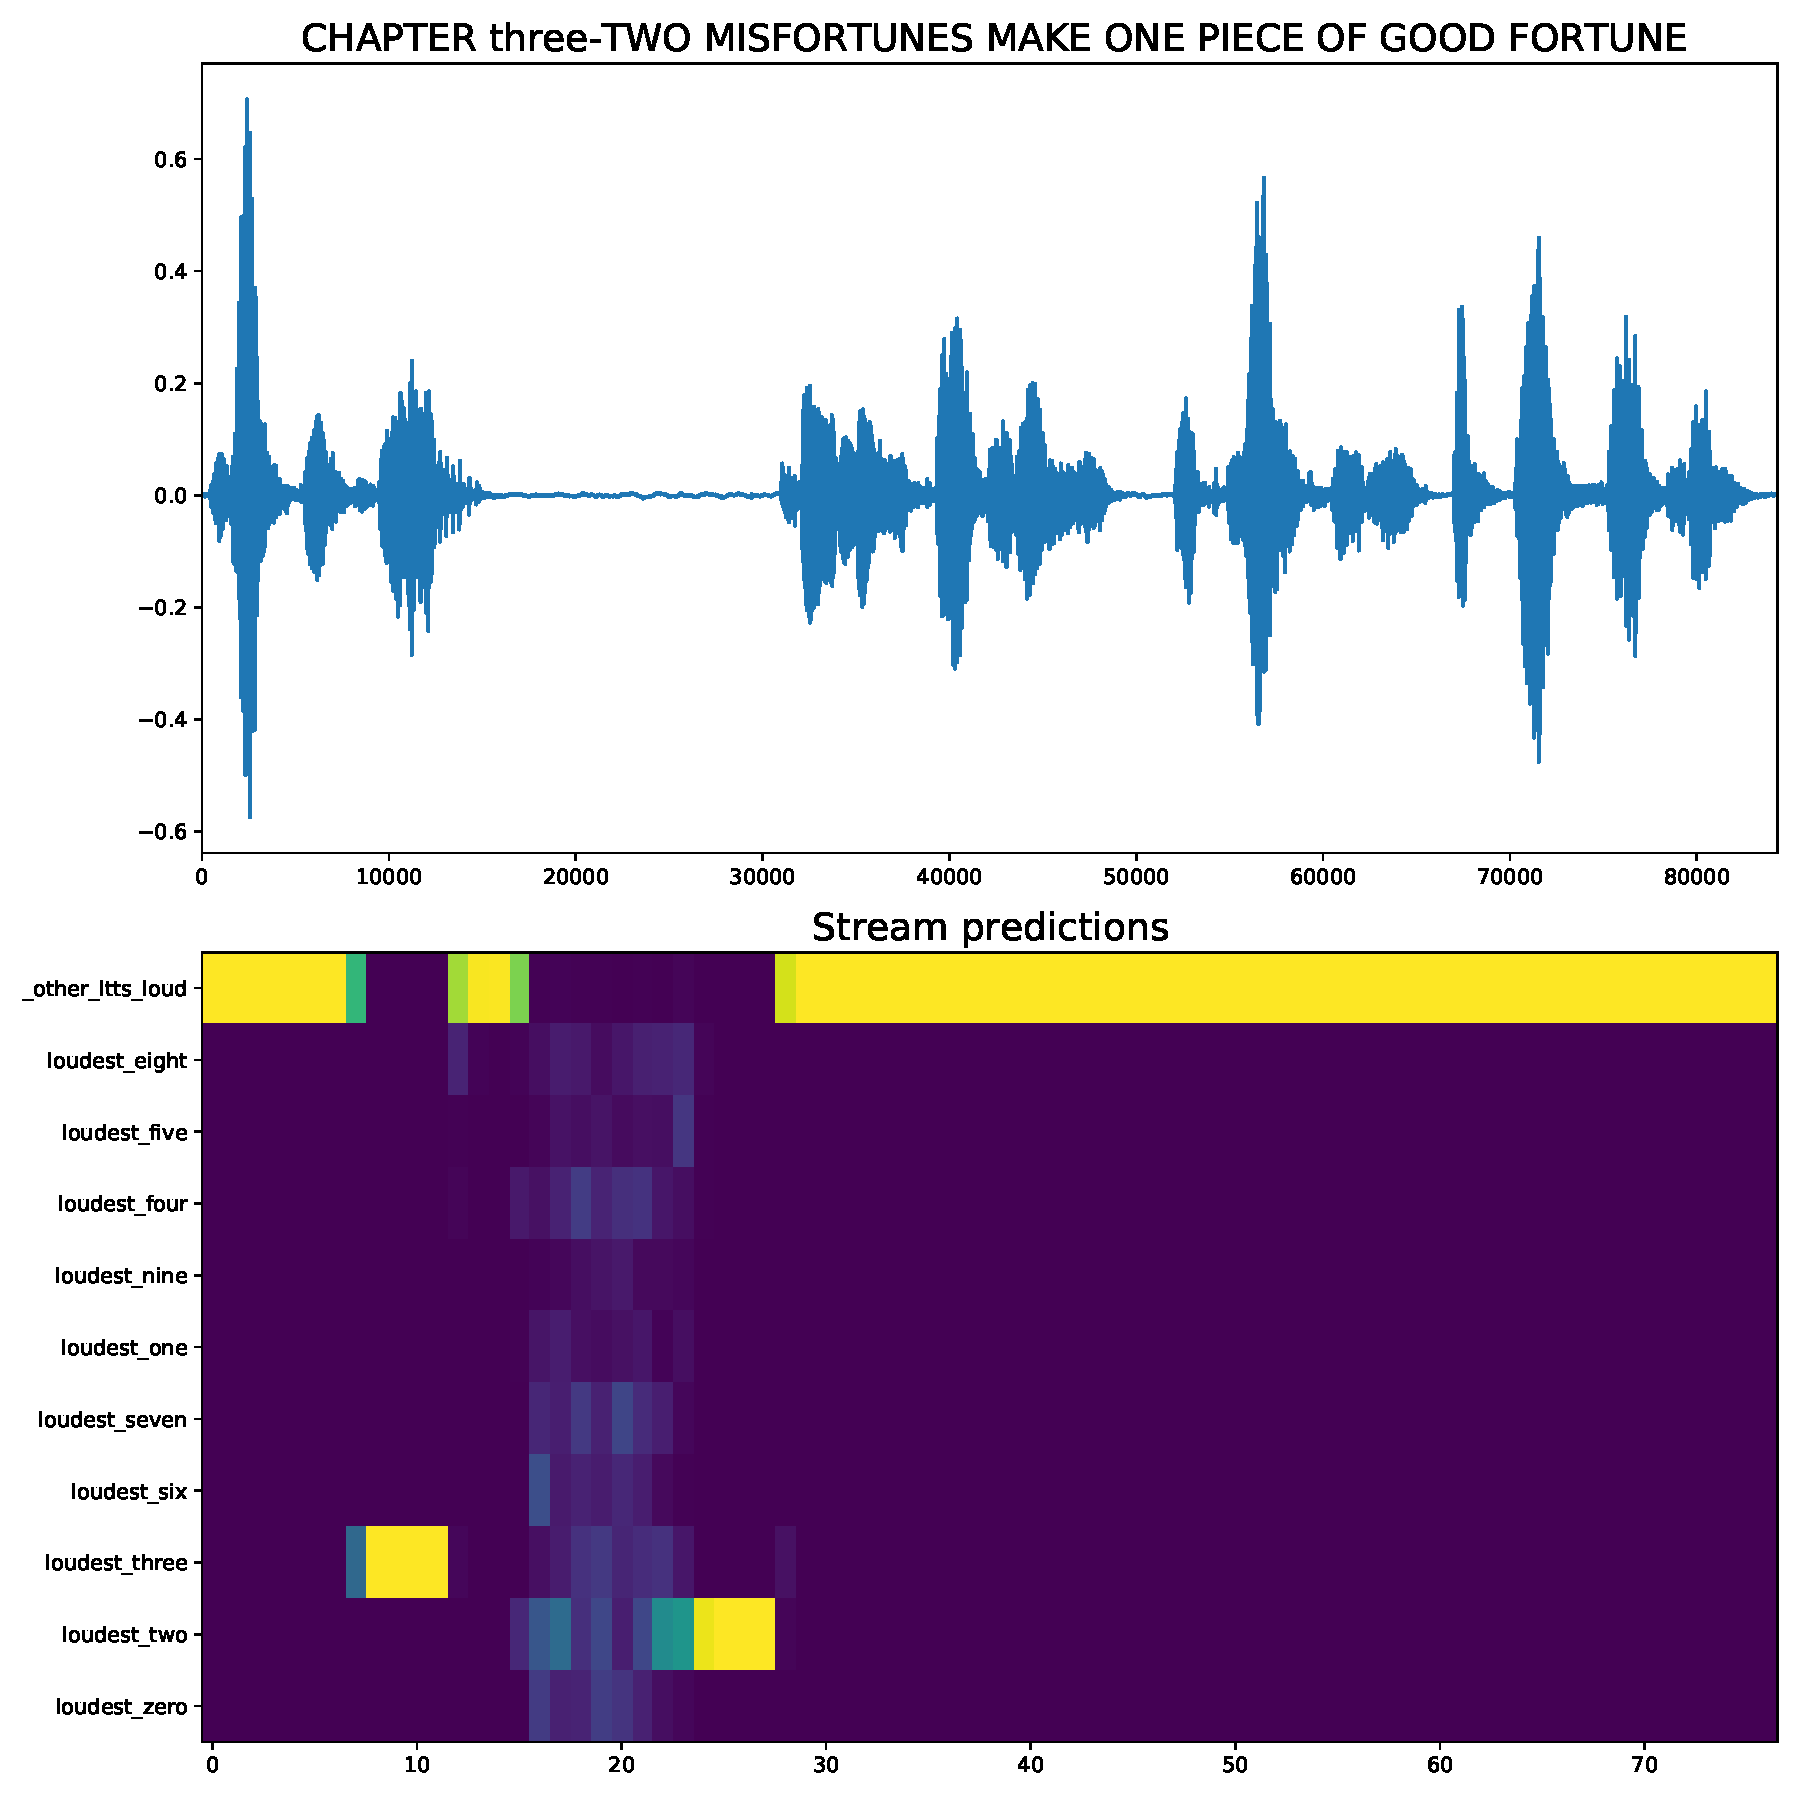
\includegraphics[width=0.9\linewidth]{stream2_attention_ltts_meL04_LTnumLS_19.pdf}
    \caption{Stream 19}%
    \label{fig:stream_attention_ltts_meL04_LTnumLS_19}
\end{figure}

% Attention vs Simple vs AreaNet vs VerticalAreaNet

TODO: Compare inference time, model size

TODO: Show stream with silence label

% Little difference in performance


% !TEX root = report.tex

\section{Concluding Remarks}
\label{sec:conclusions}

% A gripping conclusion
The task of identifying a command in a single audio sample has been successfully
solved, with varying degree of accuracy, by every architecture tested.

%
It was proved that the attention mechanism is not very effective when dealing
with spectrogram images.
%
A possible reason is that the relevant portion is already very clear, while in
the background regions that do not contain sound the spectrogram is very
uniform and with very low values.
%
In these regions, the convolutional filters already have very low output
values, so using the attention mechanism to further emphasize the relevant
portions does not help, but can instead hinder the learning by sometime
mistakenly dimming useful regions of the spectrogram.

% further work
Further works might focus on different types of attention, and the performance
of SimpleNet and AreaNet should be evaluated on standard image classification
datasets, such as ImageNet.
%
A more complex dataset might provide an insight to whether the proposed
attention mechanism is capable of learning to spot useful features when faced
with more evenly distributed input images, where the interesting part is not
immediately clear.
% can I spot the beak of the heron or do I just learn that the center is useful?

%
Having proved the effectiveness of SimpleNets, a transfer learning approach
that builds the AreaNet by using an SimpleNet already trained on the same task
as the final block (that is not modified in the first stage of learning) might
help, as the model only has to learn to spot the relevant portion of the data
in order to maximize the SimpleNet performance.
% And can that extractor be reused on a different task.

Yet another approach might consist in training the attention weight extractor
by using known object bounding boxes, making the model predict the boxes
instead of the image class, then using the predictions to weigh the input.

% TODO: after all learning attention weights is an *unsupervised* task
% as we do not know which regions are useful
% using object bounding boxes might be interesting first train the general
% feature extractor on loss measured against the boxes
% 0000000000
% 0001111000
% 0001111000
% 0000000000
% then use that to weigh the images

Regarding the methodology used, a definite improvement would be using existing
frameworks for hyper-parameter tuning, such as Hypertune, readily available
with Keras Tuner library. A very interesting approach is Hyperband, that trains
every model built from the hyper-parameter grid for a few epochs, then prunes
the set of models, only keeping the best performing ones.

% TODO also much better preprocessing pipeline in ImageNetGenerator

% The methodical hyper-parameter analysis done while writing the report was very
% informative, and while the plots confirmed what I believed to be the best
% combinations, they gave me a couple of ideas regarding some explorations that I
% had missed.


\bibliography{biblio}
\bibliographystyle{ieeetr}

\section{Appendix}
\label{sec:appendix}

% https://tex.stackexchange.com/a/210378
\renewcommand{\thefigure}{A.\arabic{figure}}
\setcounter{figure}{0}

\renewcommand{\thetable}{A.\arabic{table}}
\setcounter{table}{0}

Several large tables and figures are here for ease of reading.

\begin{figure}[t!]
    \centering
    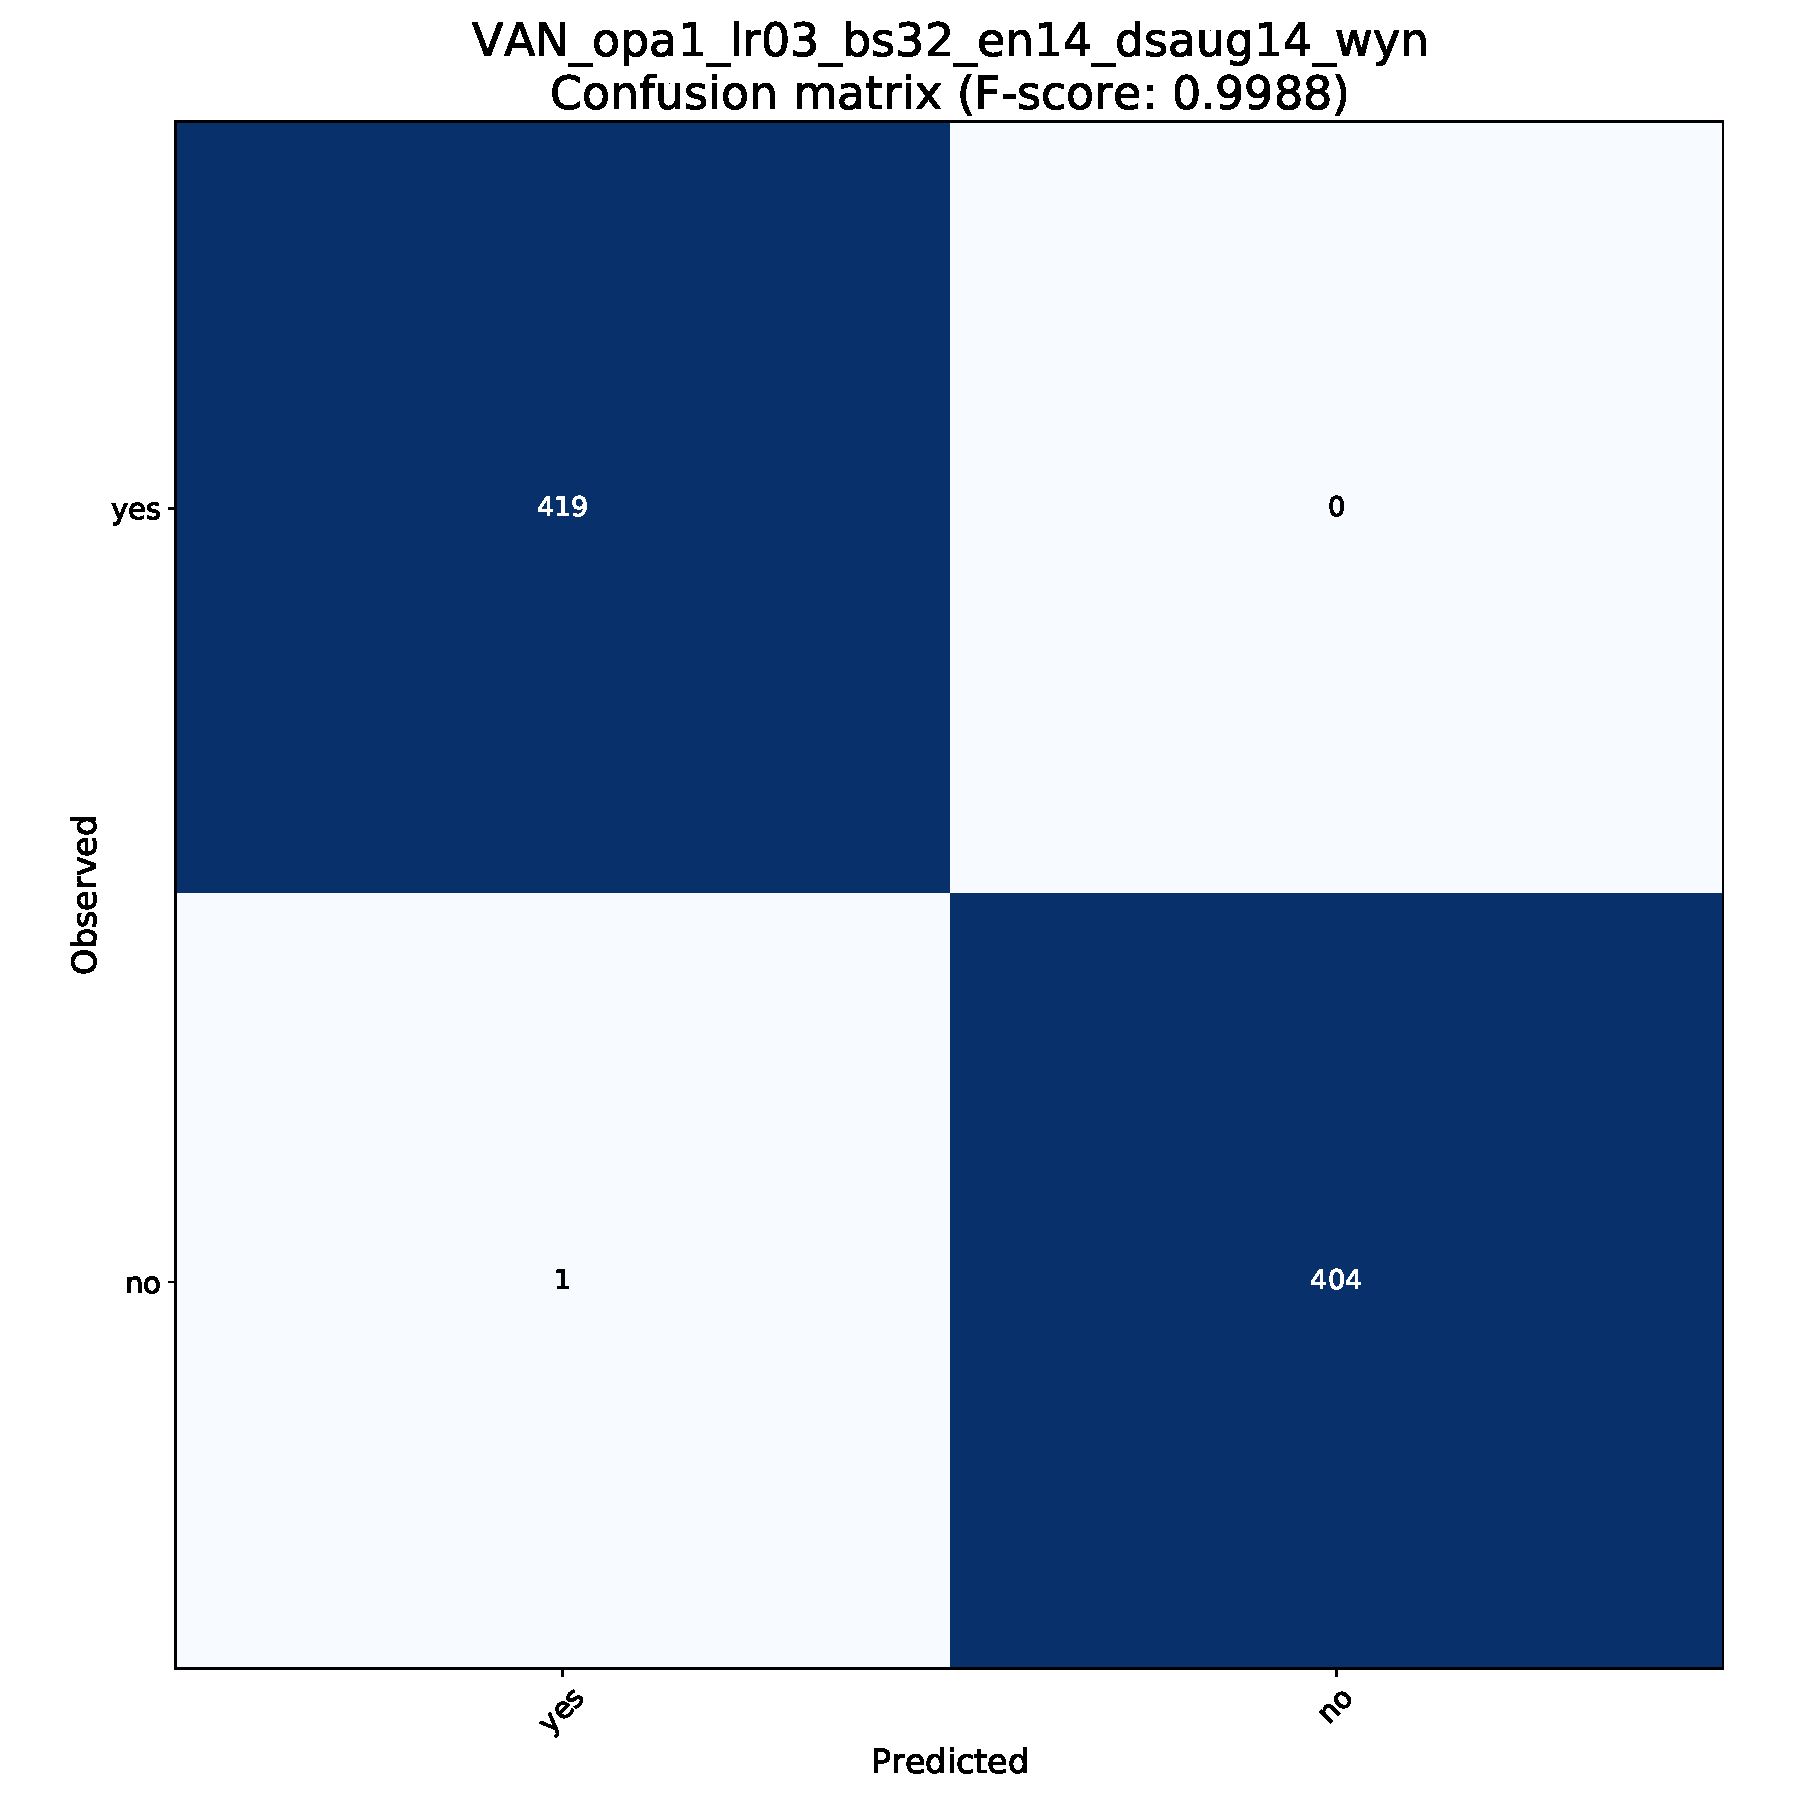
\includegraphics[width=0.9\linewidth]{VAN_opa1_lr03_bs32_en14_dsaug14_wyn_cm.pdf}
    \caption{VAN opa1 lr03 bs32 en14 dsaug14 wyn cm}%
    \label{fig:VAN_opa1_lr03_bs32_en14_dsaug14_wyn_cm}
\end{figure}

% \begin{figure}[t!]
%     \centering
%     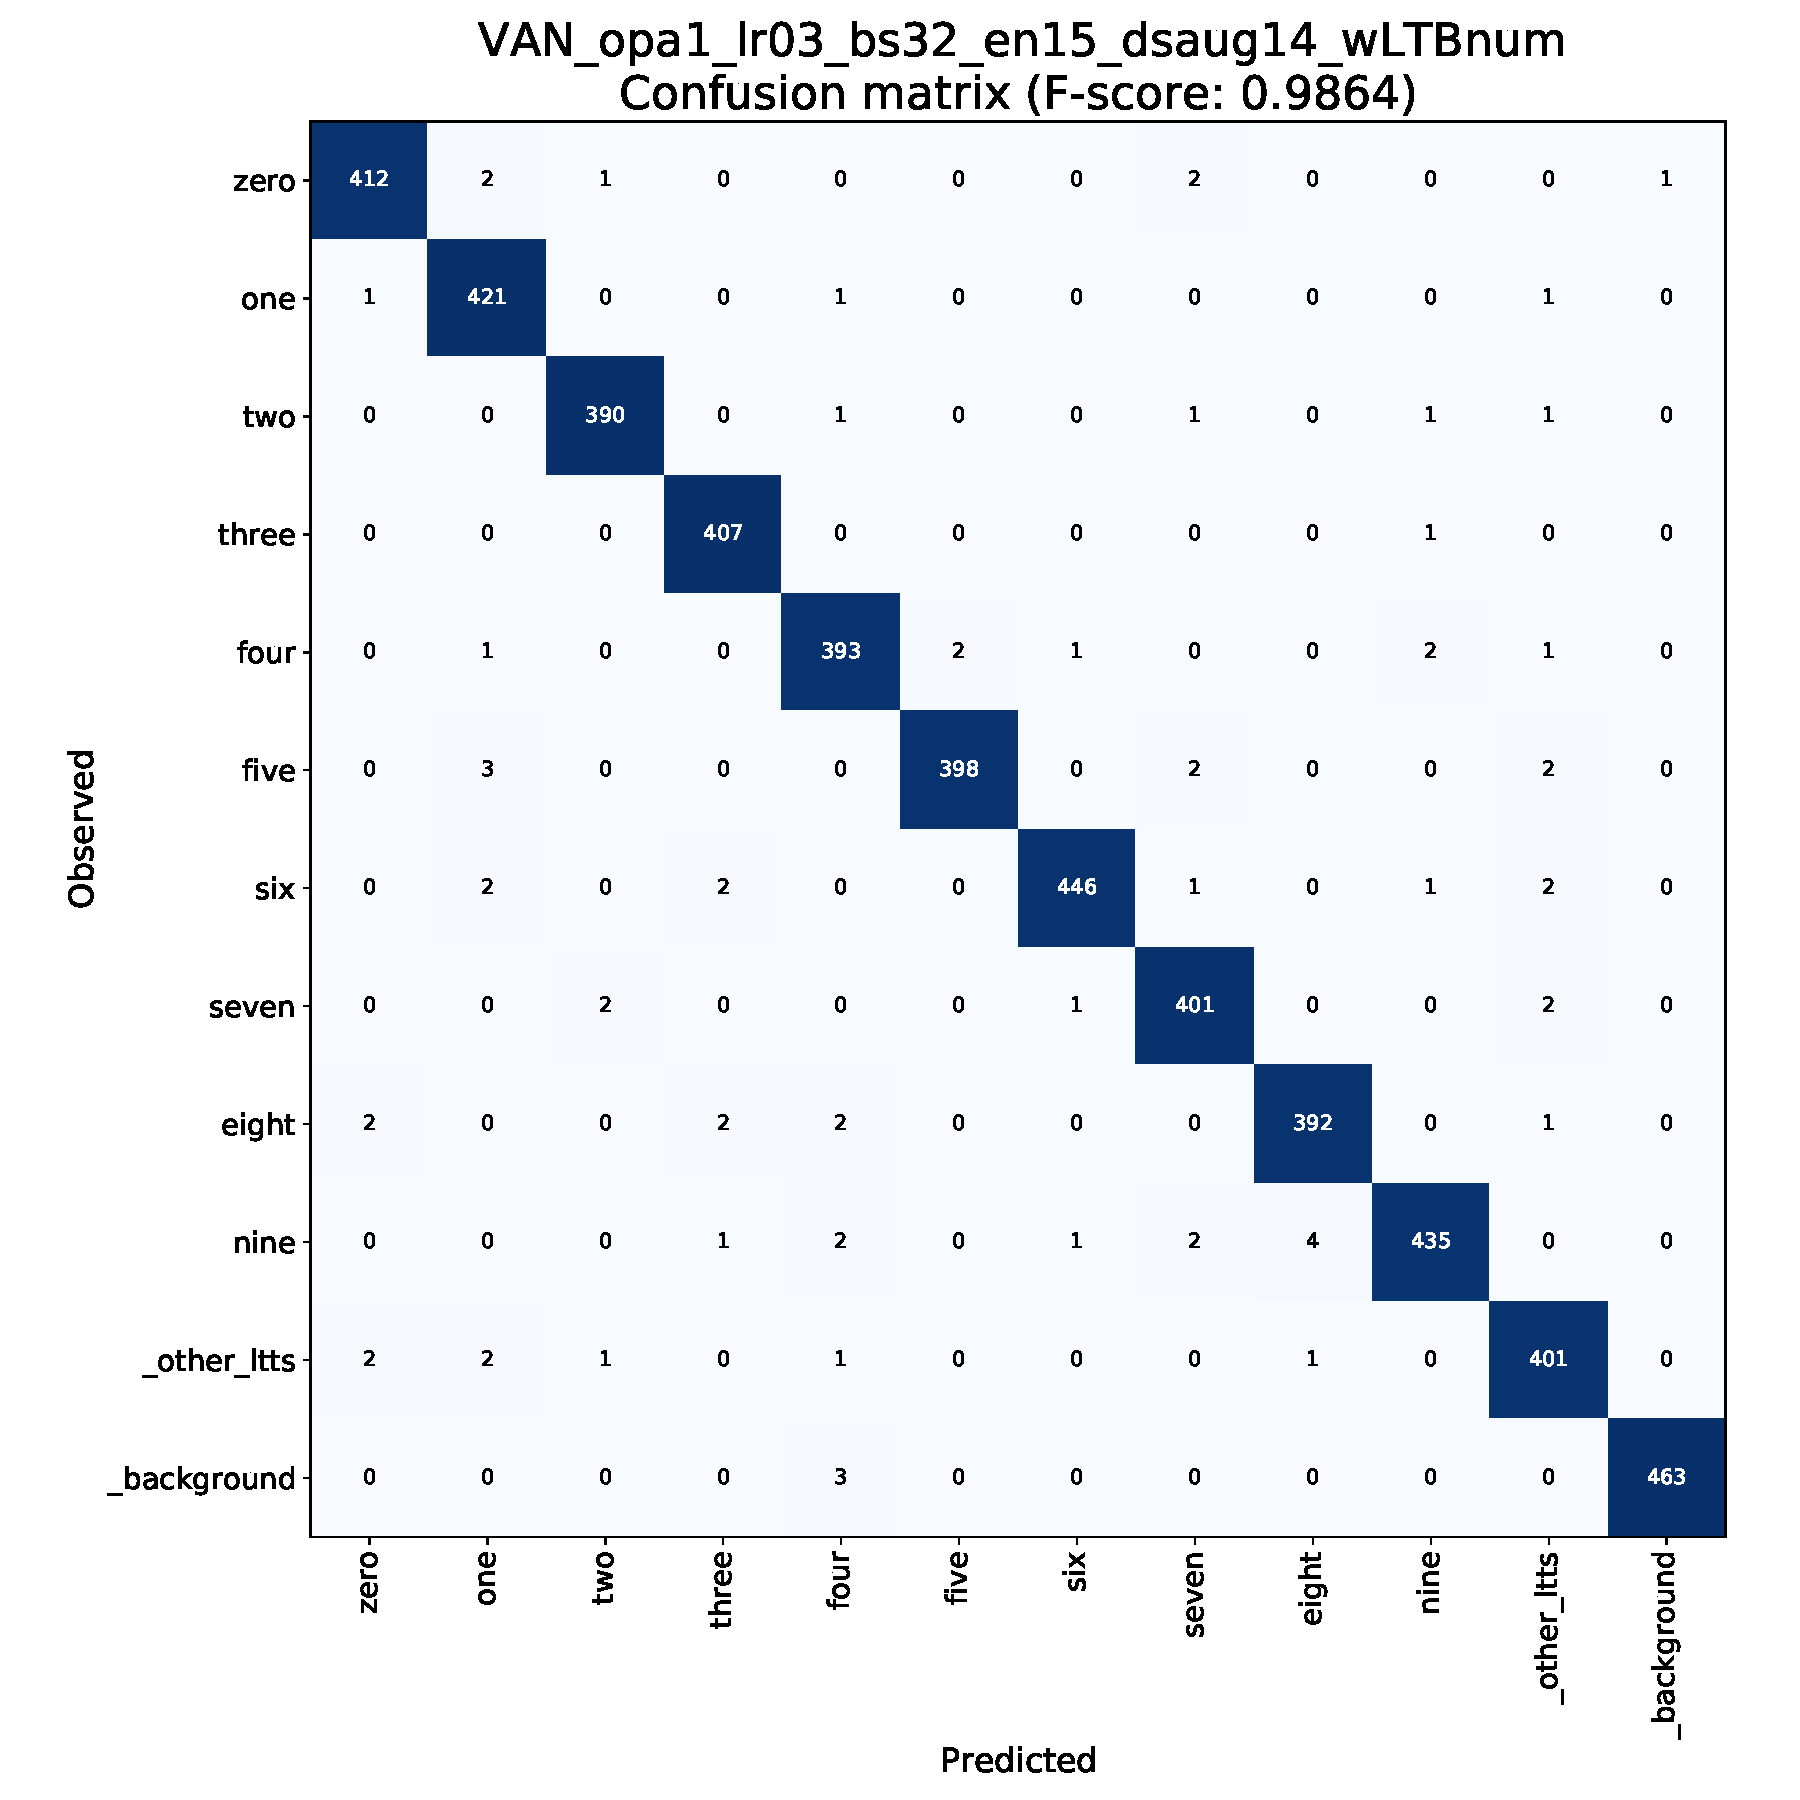
\includegraphics[width=0.9\linewidth]{VAN_opa1_lr03_bs32_en15_dsaug14_wLTBnum_cm.pdf}
%     \caption{VAN opa1 lr03 bs32 en15 dsaug14 wLTBnum cm}%
%     \label{fig:VAN_opa1_lr03_bs32_en15_dsaug14_wLTBnum_cm}
% \end{figure}

\begin{figure*}[t!]
    \centering
    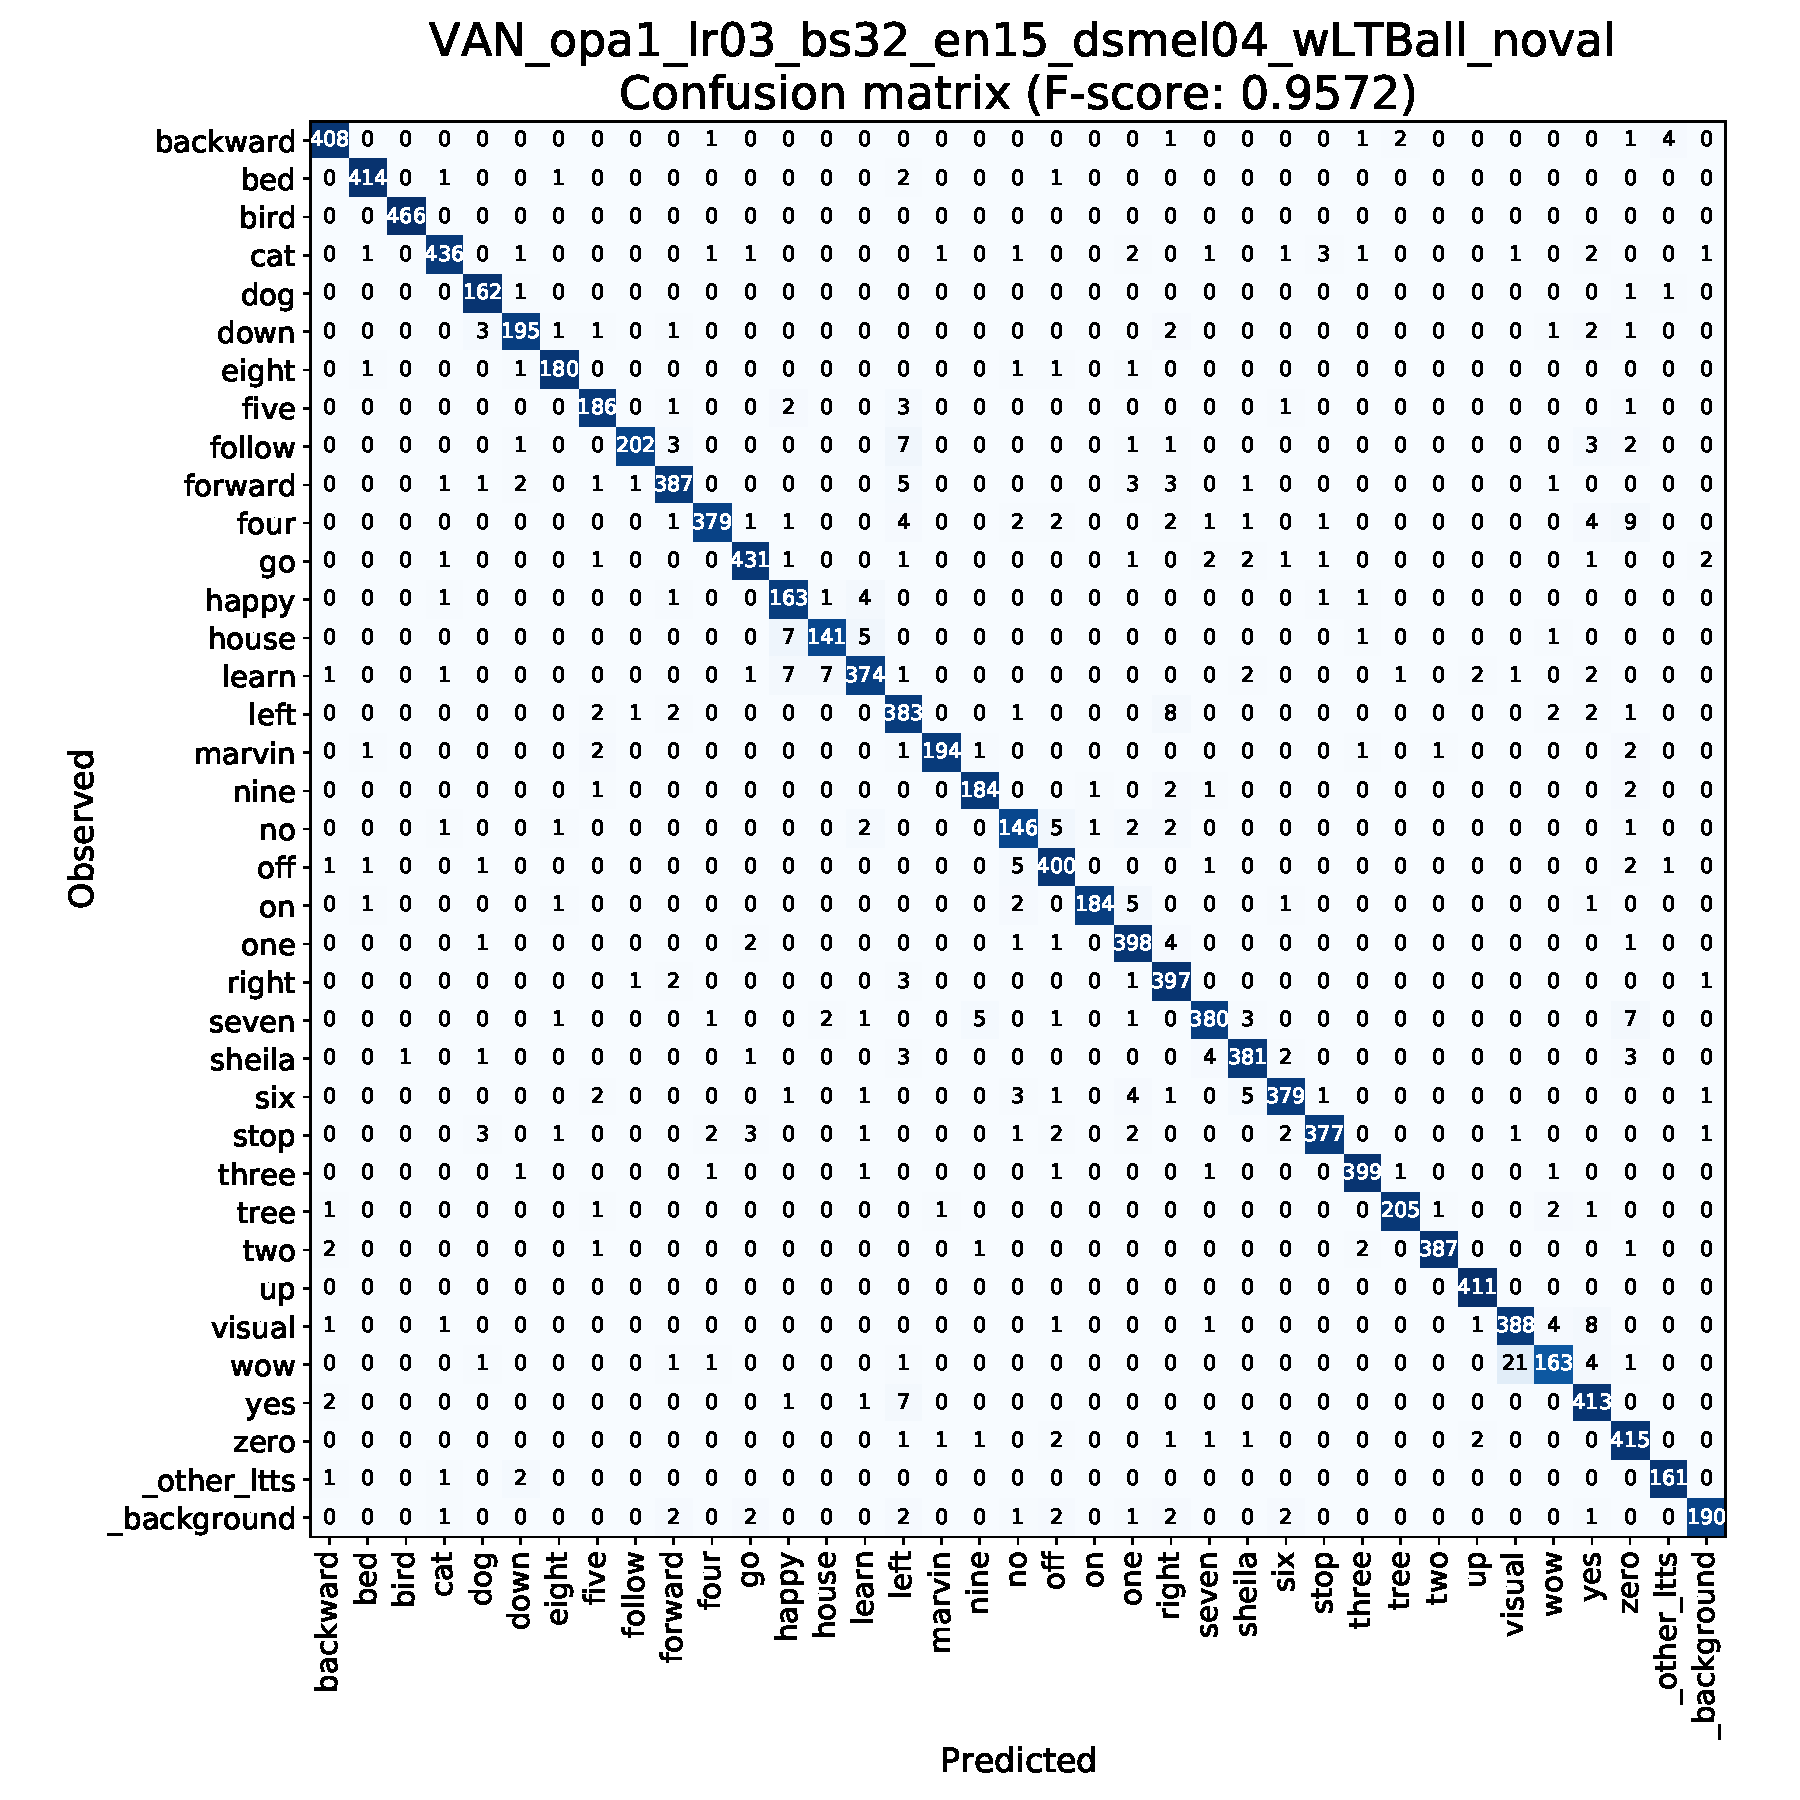
\includegraphics[width=0.9\linewidth]{VAN_opa1_lr03_bs32_en15_dsmel04_wLTBall_noval_cm.pdf}
    \caption{VAN opa1 lr03 bs32 en15 dsmel04 wLTBall noval cm}%
    \label{fig:VAN_opa1_lr03_bs32_en15_dsmel04_wLTBall_noval_cm}
\end{figure*}

\begin{figure*}[t!]
    \centering
    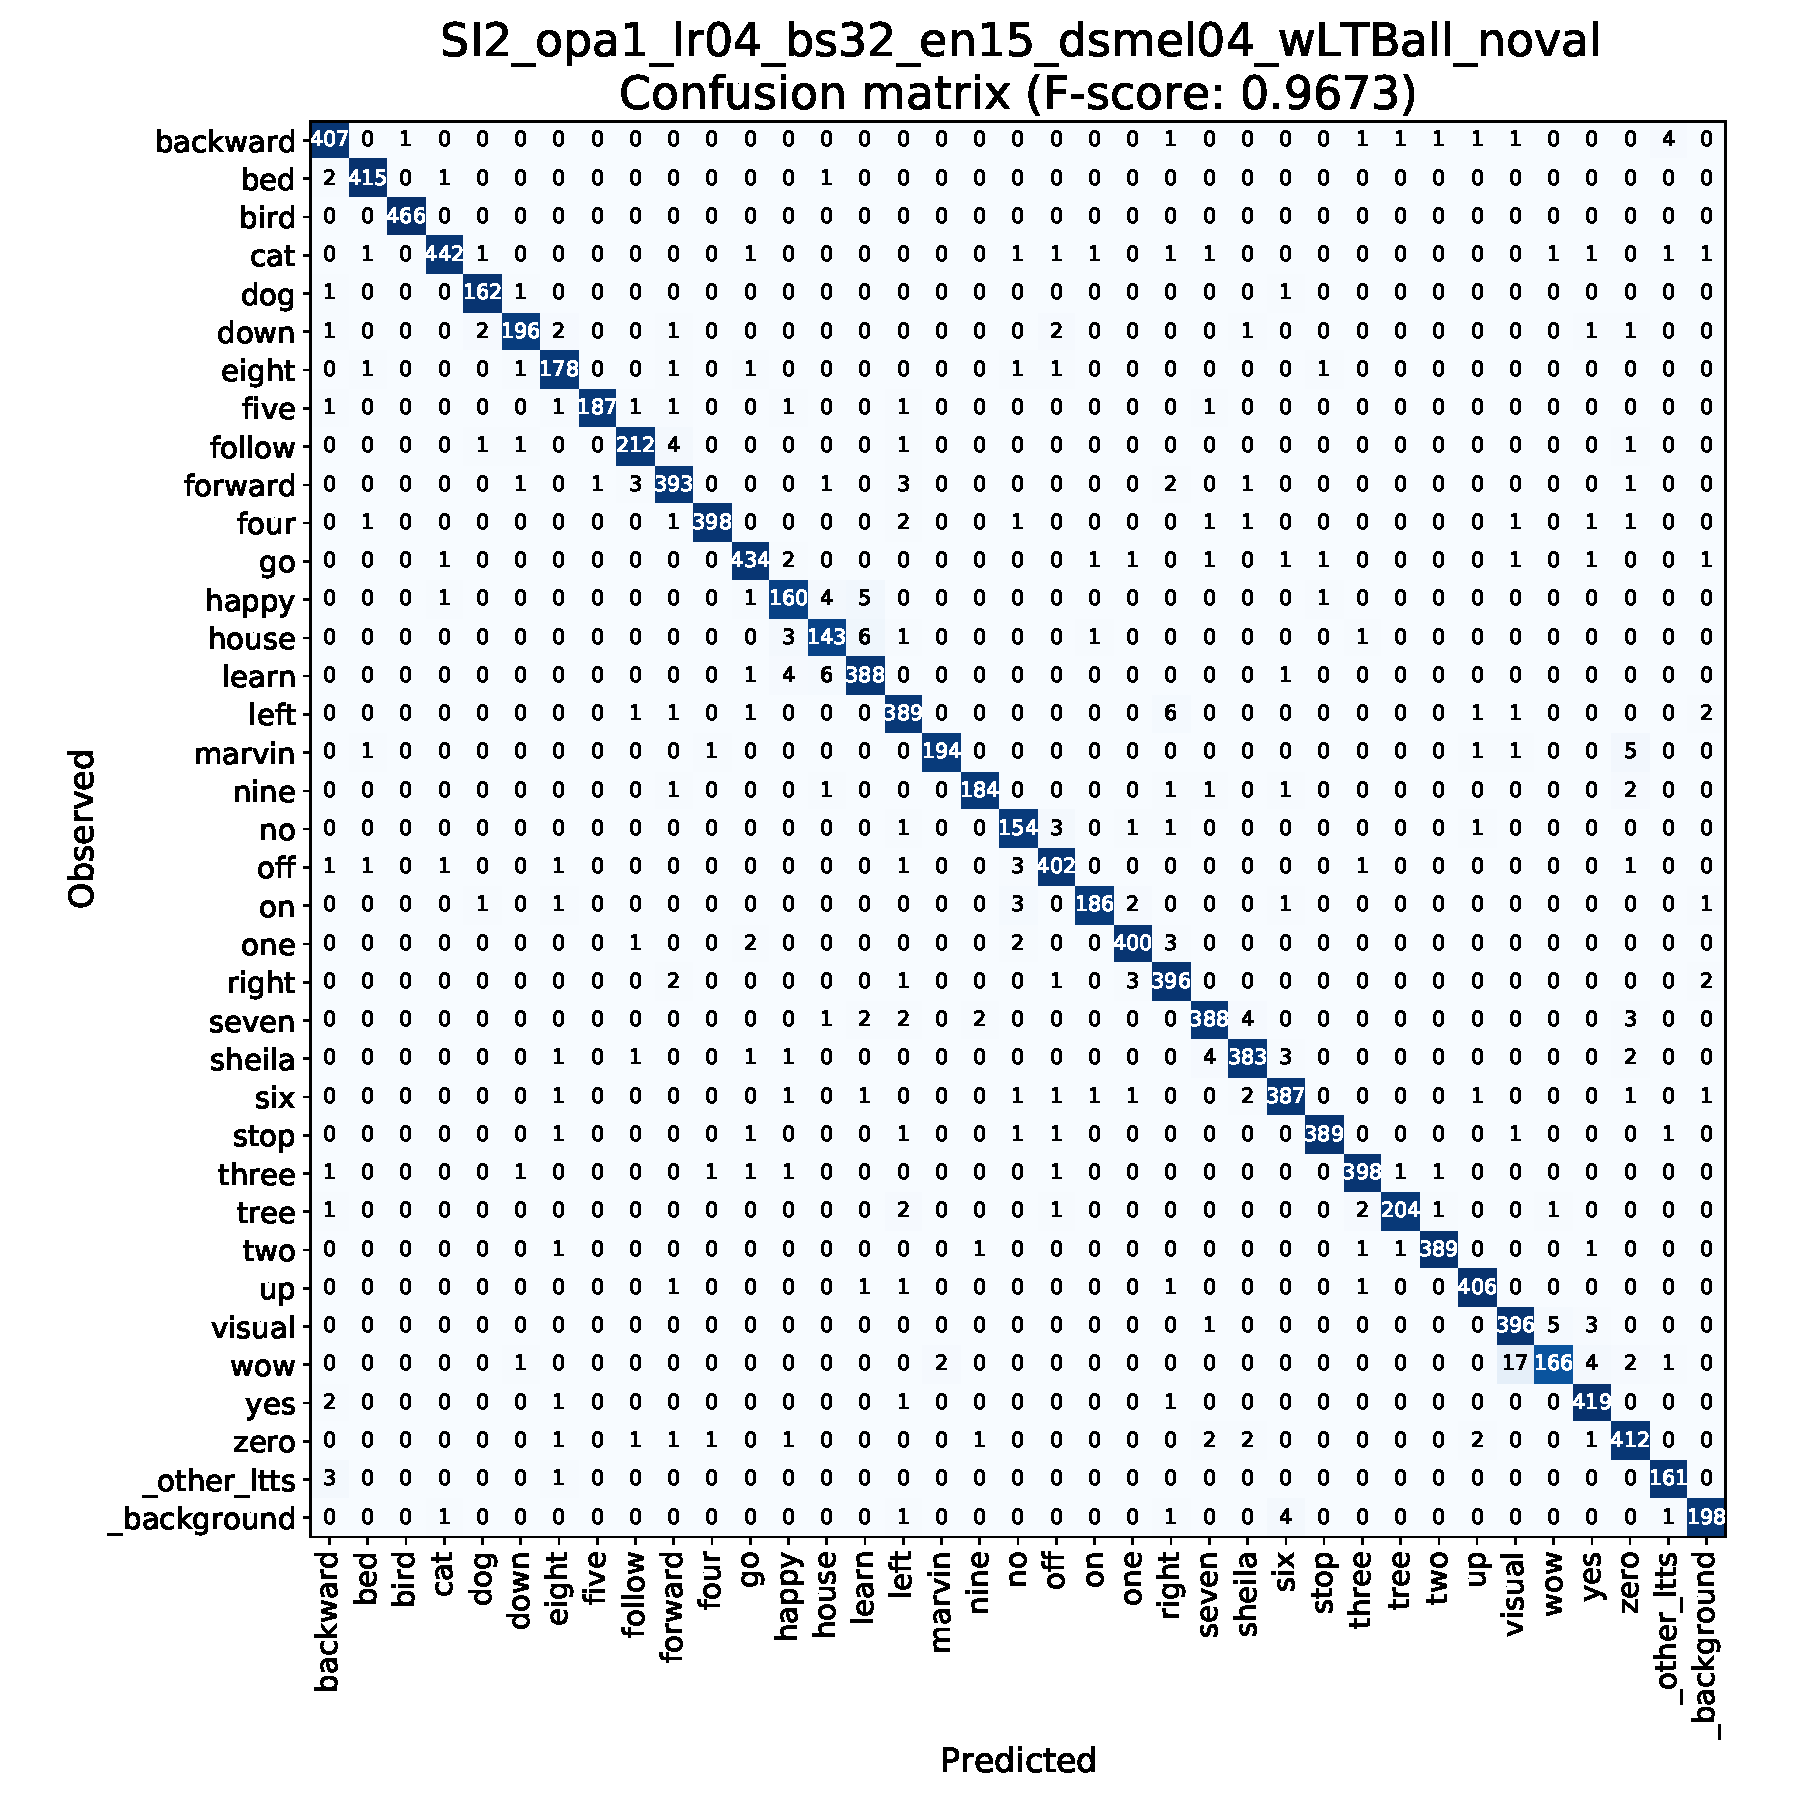
\includegraphics[width=0.9\linewidth]{SI2_opa1_lr04_bs32_en15_dsmel04_wLTBall_noval_cm.pdf}
    \caption{SI2 opa1 lr04 bs32 en15 dsmel04 wLTBall noval cm}%
    \label{fig:SI2_opa1_lr04_bs32_en15_dsmel04_wLTBall_noval_cm}
\end{figure*}

\begin{figure*}[t!]
    \centering
    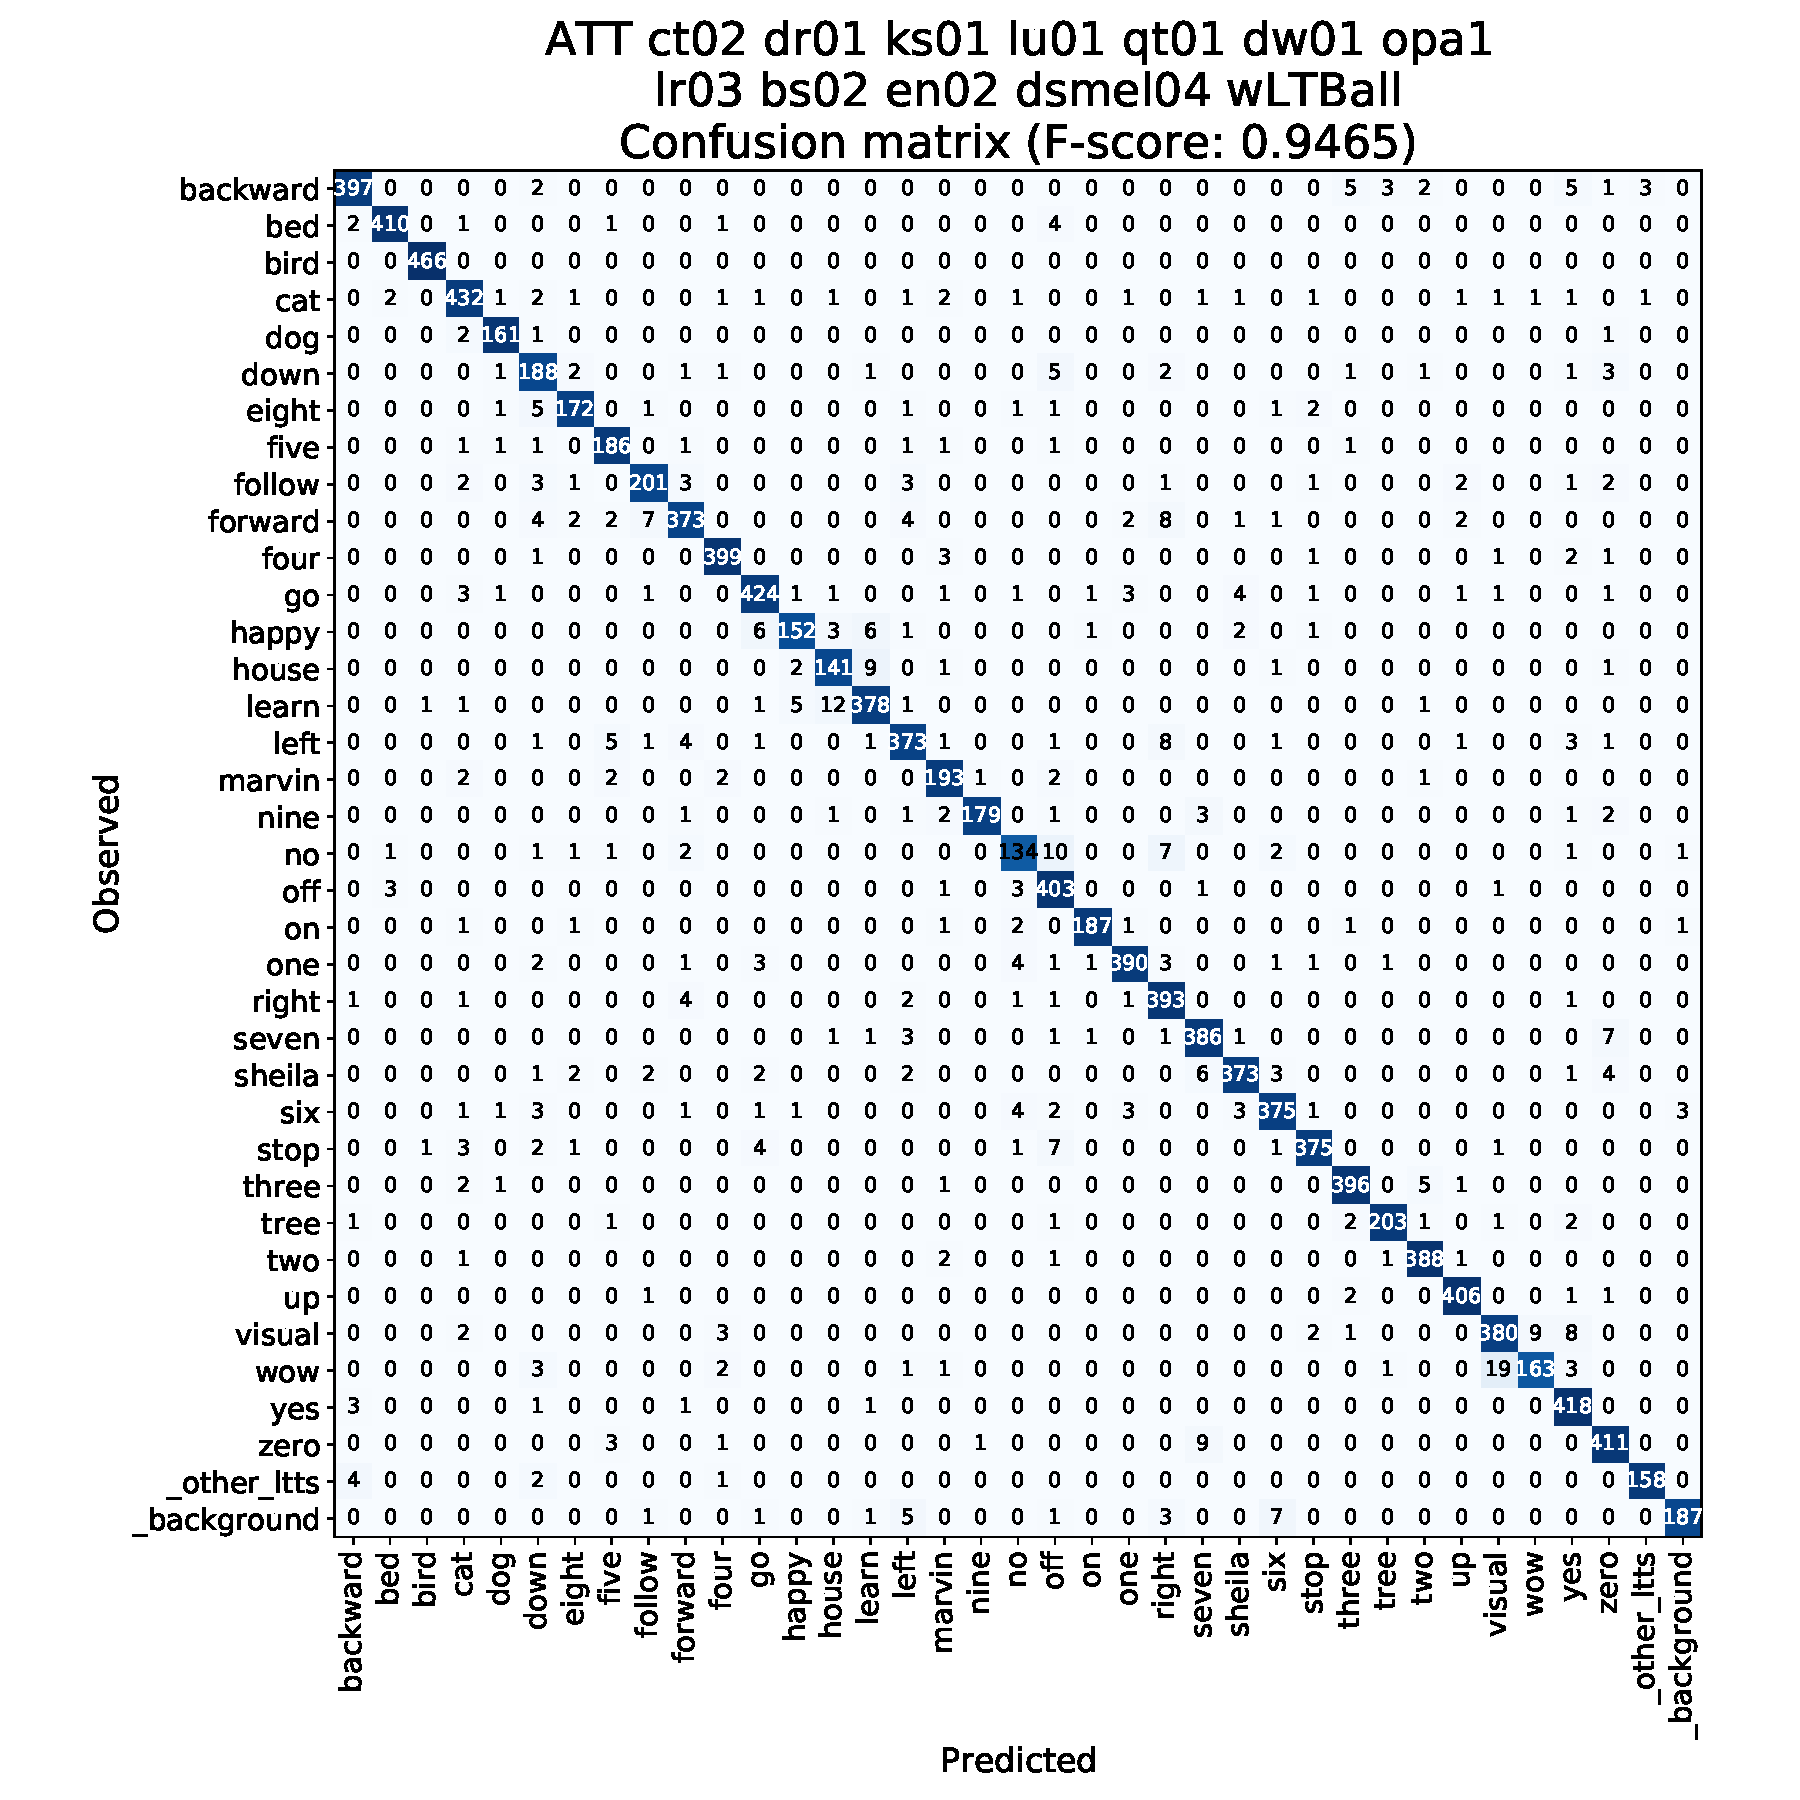
\includegraphics[width=0.9\linewidth]{ATT_ct02_dr01_ks01_lu01_qt01_dw01_opa1_lr03_bs02_en02_dsmel04_wLTBall_cm.pdf}
    \caption{ATT ct02 dr01 ks01 lu01 qt01 dw01 opa1 lr03 bs02 en02 dsmel04 wLTBall cm}%
    \label{fig:ATT_ct02_dr01_ks01_lu01_qt01_dw01_opa1_lr03_bs02_en02_dsmel04_wLTBall_cm}
\end{figure*}

% https://stackoverflow.com/a/15221702/2237151
% find . -type d -print0 | while read -d '' -r dir; do files=("$dir"/*); printf "%s & %d\n" "$dir" "${#files[@]}"; done

\begin{table}[h!]
    \centering
    \caption{Task composition.
    Each task is expanded by adding the
    \texttt{\_other\_ltts}
    category,
    and is referred as
    \texttt{LT\_\{task\_key\}}.
    The second column shows the number of samples for that word.
    }
    \label{tab:task_word_composition}
    \begin{tabular}{|c|c|ccccccc|}
        \hline
        Words & $\#$          &f1 &f2 &dir&num&k1 &w2 &all \\
        \hline
        backward & 1664       &   & x & x &   &   &   & x  \\
        bed & 2014            &   &   &   &   &   &   & x  \\
        bird & 2064           &   &   &   &   &   &   & x  \\
        cat & 2031            &   &   &   &   &   &   & x  \\
        \hline
        dog & 2128            &   &   &   &   &   &   & x  \\
        down & 3917           &   &   & x &   & x & x & x  \\
        eight & 3787          &   & x &   & x &   & x & x  \\
        five & 4052           &   &   &   & x &   & x & x  \\
        \hline
        follow & 1579         &   &   &   &   &   &   & x  \\
        forward & 1557        &   &   & x &   &   &   & x  \\
        four & 3728           &   &   &   & x &   & x & x  \\
        go & 3880             &   & x &   &   & x & x & x  \\
        \hline
        happy & 2054          & x &   &   &   &   &   & x  \\
        house & 2113          &   &   &   &   &   &   & x  \\
        learn & 1575          & x &   &   &   &   &   & x  \\
        left & 3801           &   &   & x &   & x & x & x  \\
        \hline
        marvin & 2100         &   &   &   &   &   &   & x  \\
        nine & 3934           &   &   &   & x &   & x & x  \\
        no & 3941             &   &   &   &   & x & x & x  \\
        off & 3745            &   &   &   &   & x & x & x  \\
        \hline
        on & 3845             &   &   &   &   & x & x & x  \\
        one & 3890            &   &   &   & x &   & x & x  \\
        right & 3778          &   &   & x &   & x & x & x  \\
        seven & 3998          &   &   &   & x &   & x & x  \\
        \hline
        sheila & 2022         &   &   &   &   &   &   & x  \\
        six & 3860            &   &   &   & x &   & x & x  \\
        stop & 3872           &   &   &   &   & x & x & x  \\
        three & 3727          &   &   &   & x &   & x & x  \\
        \hline
        tree & 1759           &   &   &   &   &   &   & x  \\
        two & 3880            &   &   &   & x &   & x & x  \\
        up & 3723             &   &   & x &   & x & x & x  \\
        visual & 1592         & x &   &   &   &   &   & x  \\
        \hline
        wow & 2123            & x &   &   &   &   &   & x  \\
        yes & 4044            &   & x &   &   & x & x & x  \\
        zero & 4052           &   &   &   & x &   & x & x  \\
        \_other\_ltts & 4954  &   &   &   &   &   &   &    \\
        \hline
    \end{tabular}
\end{table}

\begin{table}[h!]
% \begin{table}[H]
    \centering
    \caption{
    Values used to generate the mel spectrograms. The dataset ``mela1'' also
has the parameter \texttt{fmin}$=40$.}
    \label{tab:mel_values}
    \begin{tabular}{|c|cccc|}
        \hline
        % name & \texttt{n\_mel} & \texttt{n\_fft} & \texttt{hop\_length} & shape \\
        name & n\_mel & n\_fft & hop\_length & shape \\
        \hline
        mel01 & 128 & 2048 & 512   & (128, 32) \\
        mel02 & 64  & 4096 & 1024  & (64, 16) \\
        mel03 & 64  & 2048 & 512   & (64, 32) \\
        mel04 & 64  & 1024 & 256   & (64, 64) \\
        mel05 & 128 & 1024 & 128   & (128, 128) \\
        mel06 & 128 & 1024 & 256   & (128, 64) \\
        mel07 & 128 & 2048 & 256   & (128, 64) \\
        mel08 & 128 & 512  & 256   & (128, 64) \\
        mel09 & 128 & 512  & 128   & (128, 128) \\
        mel10 & 128 & 2048 & 128   & (128, 128) \\
        mel11 & 128 & 256  & 128   & (128, 128) \\
        mel12 & 128 & 4096 & 256   & (128, 64) \\
        mel13 & 128 & 512  & 256   & (128, 64) \\
        mel14 & 128 & 256  & 256   & (128, 64) \\
        mel15 & 128 & 3072 & 256   & (128, 64) \\
        mela1 & 80  & 1024 & 128   & (80, 128) \\
        \hline
    \end{tabular}
\end{table}

% \begin{table}[H]
\begin{table}[h!]
    \centering
    \caption{Values used to generate the MFCC spectrograms}
    \label{tab:mfcc_values}
    \begin{tabular}{|c|cccc|}
        \hline
        % name & \texttt{n\_mfcc} & \texttt{n\_fft} & \texttt{hop\_length} & shape \\
        name & n\_mfcc & n\_fft & hop\_length & shape \\
        \hline
        mfcc01 & 20  & 2048 & 512  & (20, 32) \\
        mfcc02 & 40  & 2048 & 512  & (40, 32) \\
        mfcc03 & 40  & 2048 & 256  & (40, 64) \\
        mfcc04 & 80  & 1024 & 128  & (80, 128) \\
        mfcc05 & 10  & 4096 & 1024 & (10, 16) \\
        mfcc06 & 128 & 1024 & 128  & (128, 128) \\
        mfcc07 & 128 & 512  & 128  & (128, 128) \\
        mfcc08 & 128 & 2048 & 128  & (128, 128) \\
        \hline
    \end{tabular}
\end{table}

% \begin{table}[H]
\begin{table}[h!]
    \centering
    \caption{Values used to compose the spectrogams}
    \label{tab:compose_values}
    \begin{tabular}{|c|cc|}
        \hline
        name & left spectrogam & right spectrogam \\
        \hline
        melc1 & mel06 & mel08 \\
        melc2 & mel07 & mel12 \\
        melc3 & mel13 & mel14 \\
        melc4 & mel13 & mel15 \\
        \hline
    \end{tabular}
\end{table}

% \begin{table}[H]
\begin{table}[h!]
    \centering
    \caption{Dataset stacked to obtain a 3-channel image}
    \label{tab:ch3_values}
    \begin{tabular}{|c|ccc|}
        \hline
        tag & spec1 & spec2 & spec3 \\
        \hline
        01 & mel05  & mel09  & mel10 \\
        02 & mel05  & mel10  & mfcc07 \\
        03 & mfcc06 & mfcc07 & mfcc08 \\
        04 & mel05  & mfcc06 & melc1 \\
        05 & melc1  & melc2  & melc4 \\
        \hline
    \end{tabular}
\end{table}

\begin{table*}[h!]
    \centering
    \caption{Values used to augment the dataset. The first lines list the parameters used to compute the spectrograms.}
    \label{tab:aug_values}
    \begin{tabular}{|c|cccccc|}
        \hline
        & mel\_kwargs & n\_mel & n\_fft & hop\_length & fmin & fmax \\
        \hline
        \hline
        & mel\_01 & 64 & 1024 & 256 & 40 & 8000  \\
        & mel\_02 & 128 & 2046 & 512 & 40 & 8000  \\
        & mel\_03 & 64 & 1024 & 256 & default & default  \\
        & mel\_05 & 128 & 1024 & 128 & default & default  \\
        \hline
        \hline
        aug name & max\_time\_shifts & stretch\_rate & mel\_kwargs & num\_landmarks & max\_warp\_time & max\_warp\_freq\\
        \hline
        \hline
        aug01 &  [1600, 3200] & [0.8, 1.2] & mel\_01 & 3 & 5 & 6 \\
        \hline
        aug02 &  [] & [] & mel\_02 & 3 & 5 & 5 \\
        aug03 &  [] & [] & mel\_02 & 3 & 5 & 0 \\
        aug04 &  [] & [] & mel\_02 & 3 & 0 & 5 \\
        aug05 &  [] & [] & mel\_02 & 3 & 0 & 0 \\
        \hline
        aug06 &  [] & [] & mel\_01 & 3 & 5 & 5 \\
        aug07 &  [] & [] & mel\_01 & 3 & 5 & 0 \\
        aug08 &  [] & [] & mel\_01 & 3 & 0 & 5 \\
        aug09 &  [] & [] & mel\_01 & 3 & 0 & 0 \\
        \hline
        aug10 &  [] & [] & mel\_03 & 3 & 5 & 5 \\
        aug11 &  [] & [] & mel\_03 & 3 & 5 & 0 \\
        aug12 &  [] & [] & mel\_03 & 3 & 0 & 5 \\
        aug13 &  [] & [] & mel\_03 & 3 & 0 & 0 \\
        \hline
        aug14 &  [] & [] & mel\_03 & 4 & 2 & 2 \\
        aug15 &  [] & [] & mel\_03 & 4 & 2 & 0 \\
        aug16 &  [] & [] & mel\_03 & 4 & 0 & 2 \\
        aug17 &  [] & [] & mel\_03 & 4 & 0 & 0 \\
        \hline
        aug18 &  [] & [] & mel\_05 & 3 & 5 & 5 \\
        aug19 &  [] & [] & mel\_05 & 3 & 5 & 0 \\
        aug20 &  [] & [] & mel\_05 & 3 & 0 & 5 \\
        aug21 &  [] & [] & mel\_05 & 3 & 0 & 0 \\
        \hline
    \end{tabular}
\end{table*}


\end{document}
